\chapter{Analysis and Results}
\label{chap:results}
\chapterquote{I'm a bus}
{Darren Burton 1987--2013}

\section{Description}

This would include a detailed description of the signal and background models used and the systematics included. I would describe the statistical tools used such as hypothesis testing with a test statistic and show the results which would include exclusion limits, $p$-values and SM best fit parameters (mass, signal strength, couplings etc.). One of the important considerations of the Hgg analysis is the estimation of the background. This second part of this section will concentrate on presenting an alternate analysis which takes a completely different approach to modeling the background and cross-checks the result above.

The inclusive search range for the analysis is [110,150]. The important characteristics which define the signal are its yield relative to the SM, $\mu$, and its position, \mH.
% ---- SECTION ----
\section{Signal modelling}
\label{sec:signal_model}

  The signal \MC samples (described in Sec.~\ref{sec:mc}) are propagated through the full analysis separately for each production mechanism (\ggH,\VBF,\WH,\ZH,\ttH). Events in the samples are weighted by the relevant \SM cross section, branching ratio, the integrated luminosity and the ``detector" weight which compensates for mismodelling in the \MC such as pileup, the beamspot width and discrepancies between the efficiency in data and \MC as measured in \Zee and \Zmumugamma decays. In this way the efficiency and acceptance of the detector, selection and categorisation is mapped by the \MC samples and the total number of expected \SM signal events is given by the sum of weights of the sample. The \MC is generated separately for hypothesised Higgs' masses, \mH, in the search range of $110 \leq m_{H} \leq 150$~\GeV in steps of 5~\GeV. For any intermediate points the signal model is interpolated.

\subsection{Mass factorised analysis}
\label{sec:signal_mfm}

The diphoton invariant mass signal shape is modelled in a fully parametric way for the \MFM. A separate model, consisting of a sum of Gaussians, is constructed for each production mechanism and each event class where the two cases of right vertex and wrong (misidentified) vertex are fitted separately. The number of Gaussians used in the sum varies and can be as many as five although usually two or three provides an accurate description of the signal shape. A Gaussian sum is used because it has been found that this most accurately represents the shape of the invariant mass in signal. Many of the event classes contain a mixture of events from the resolution phase space (i.e.~there are mixtures of barrel/endcap and converted/unconverted photons) so by fitting with a sum of Gaussians these different components, which are in themselves Gaussian or close to Gaussian distributed, are accounted for. Some of the event classes for particular production mechanism contain rather low \MC statistics (for example the lepton tagged category for signal produced by gluon fusion) and so fewer Gaussians are used in these cases. Clearly one expects a low signal yield for these particular cases and so a very accurate description of the shape is unneccessary. By allowing all the parameters in the Gaussian sums to float, including the means of the different Gaussian components, one obtains a parametrisation that models both the peak and tails of the signal distribution accurately. These fits are carried out at each, \mH, where signal \MC is available and then the individual fit parameters are linearly interpolated such that the shape is defined for any \mH in the range $[110,150]$~\GeV and the model now includes a floating parameter for the mass of the Higgs which can be fit to data. The right and wrong vertex shapes are then summed, with the relative fraction of right/wrong vertex events, to give a unique signal shape model in each event class for each production process. The signal normalisation, i.e.~the expected number of \SM signal events, is obtained by linearly interpolating the efficiency $\times$ acceptance, \ea, for each event class and production process as calcualted at the \mH points for which there is \MC. The total signal shape, summed over event classes and production mechanisms, is shown in Fig.~\ref{fig:sig_shape}. The total number of expected signal events, as well as the \sigeff (minimum interval containing 68.3\% of the distribution) and the \sigFW (full with at half the maximum divided by 2.35), for each event class are shown in Table~\ref{tab:sig_shape}. This information is additonally represented diagramatically in Fig.~\ref{fig:signal_composition}.

\begin{figure}
  \begin{center}
    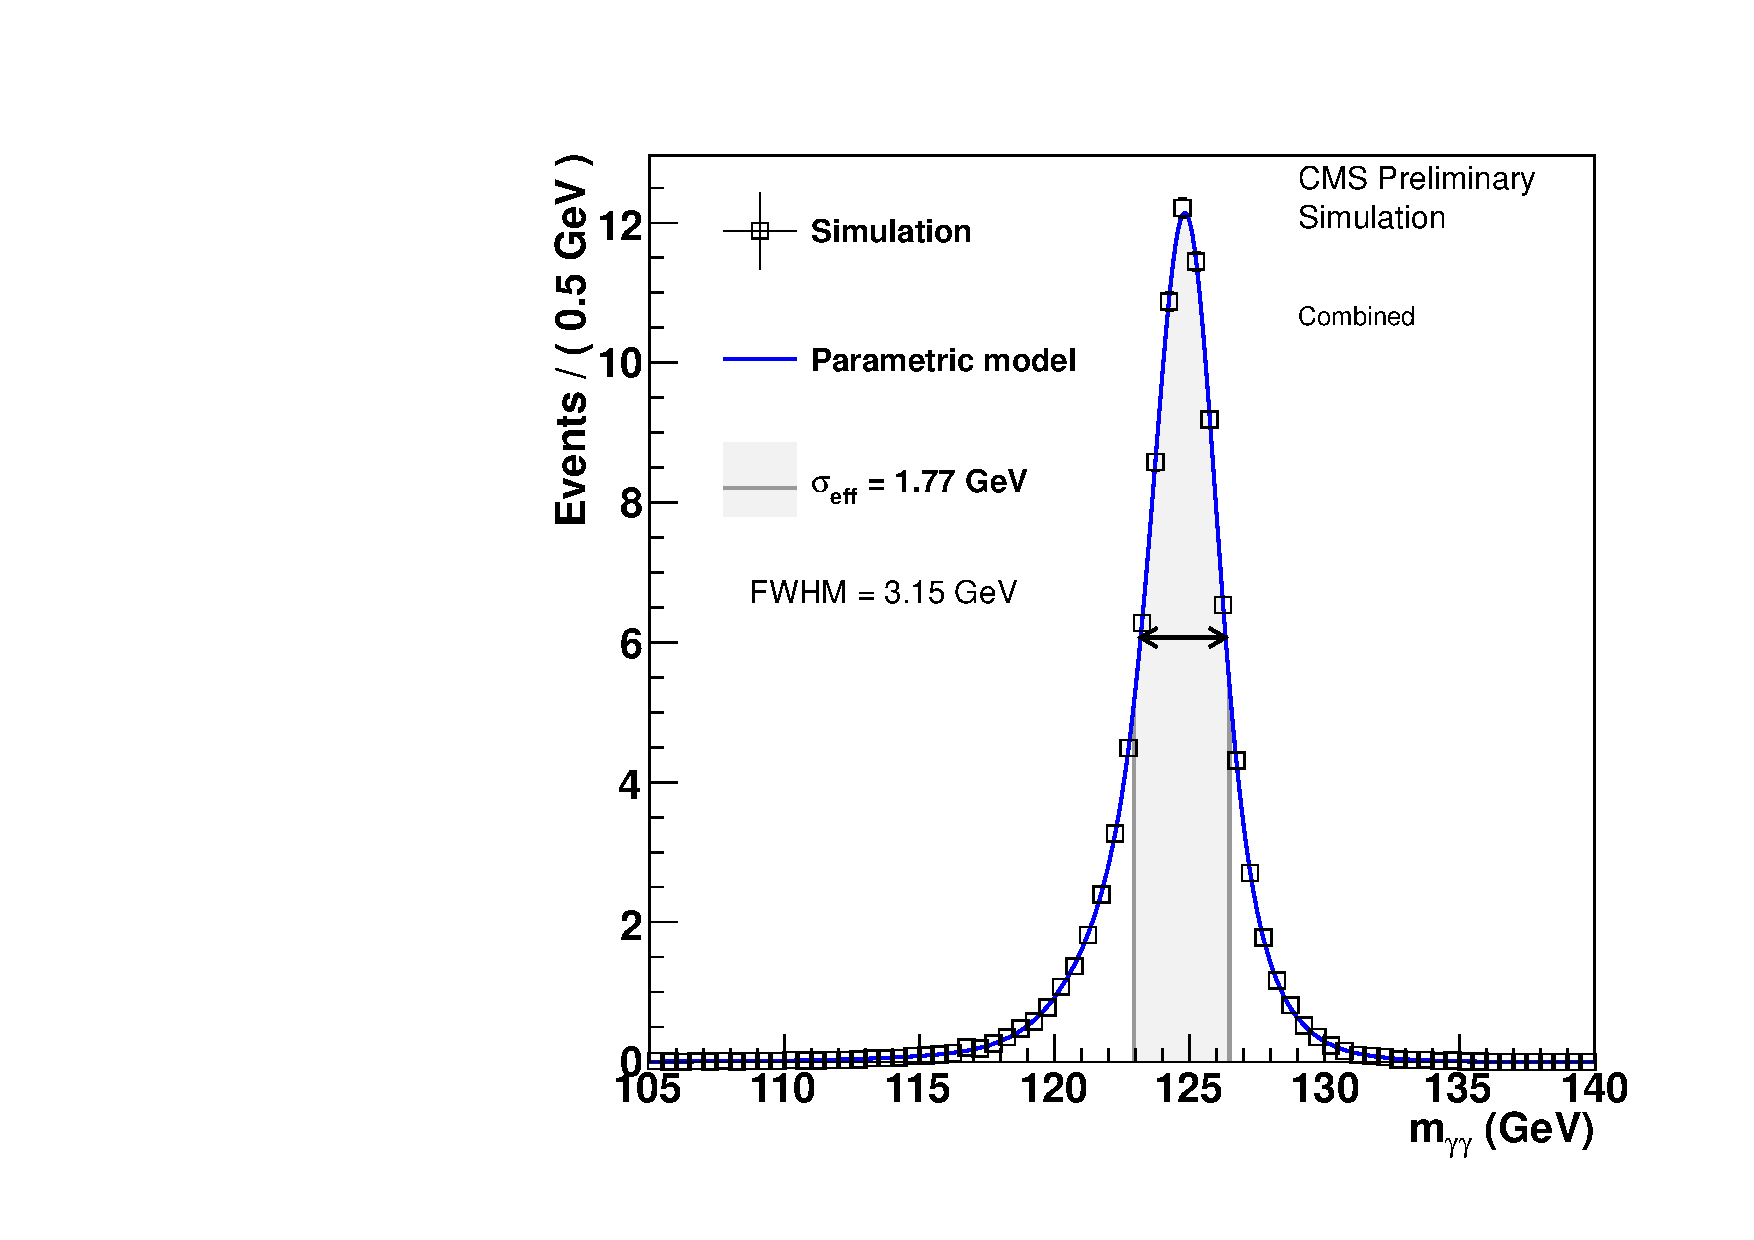
\includegraphics[width=0.49\textwidth]{ch5_anal_and_results/plots/thesis_signal_7TeV/all.pdf}
    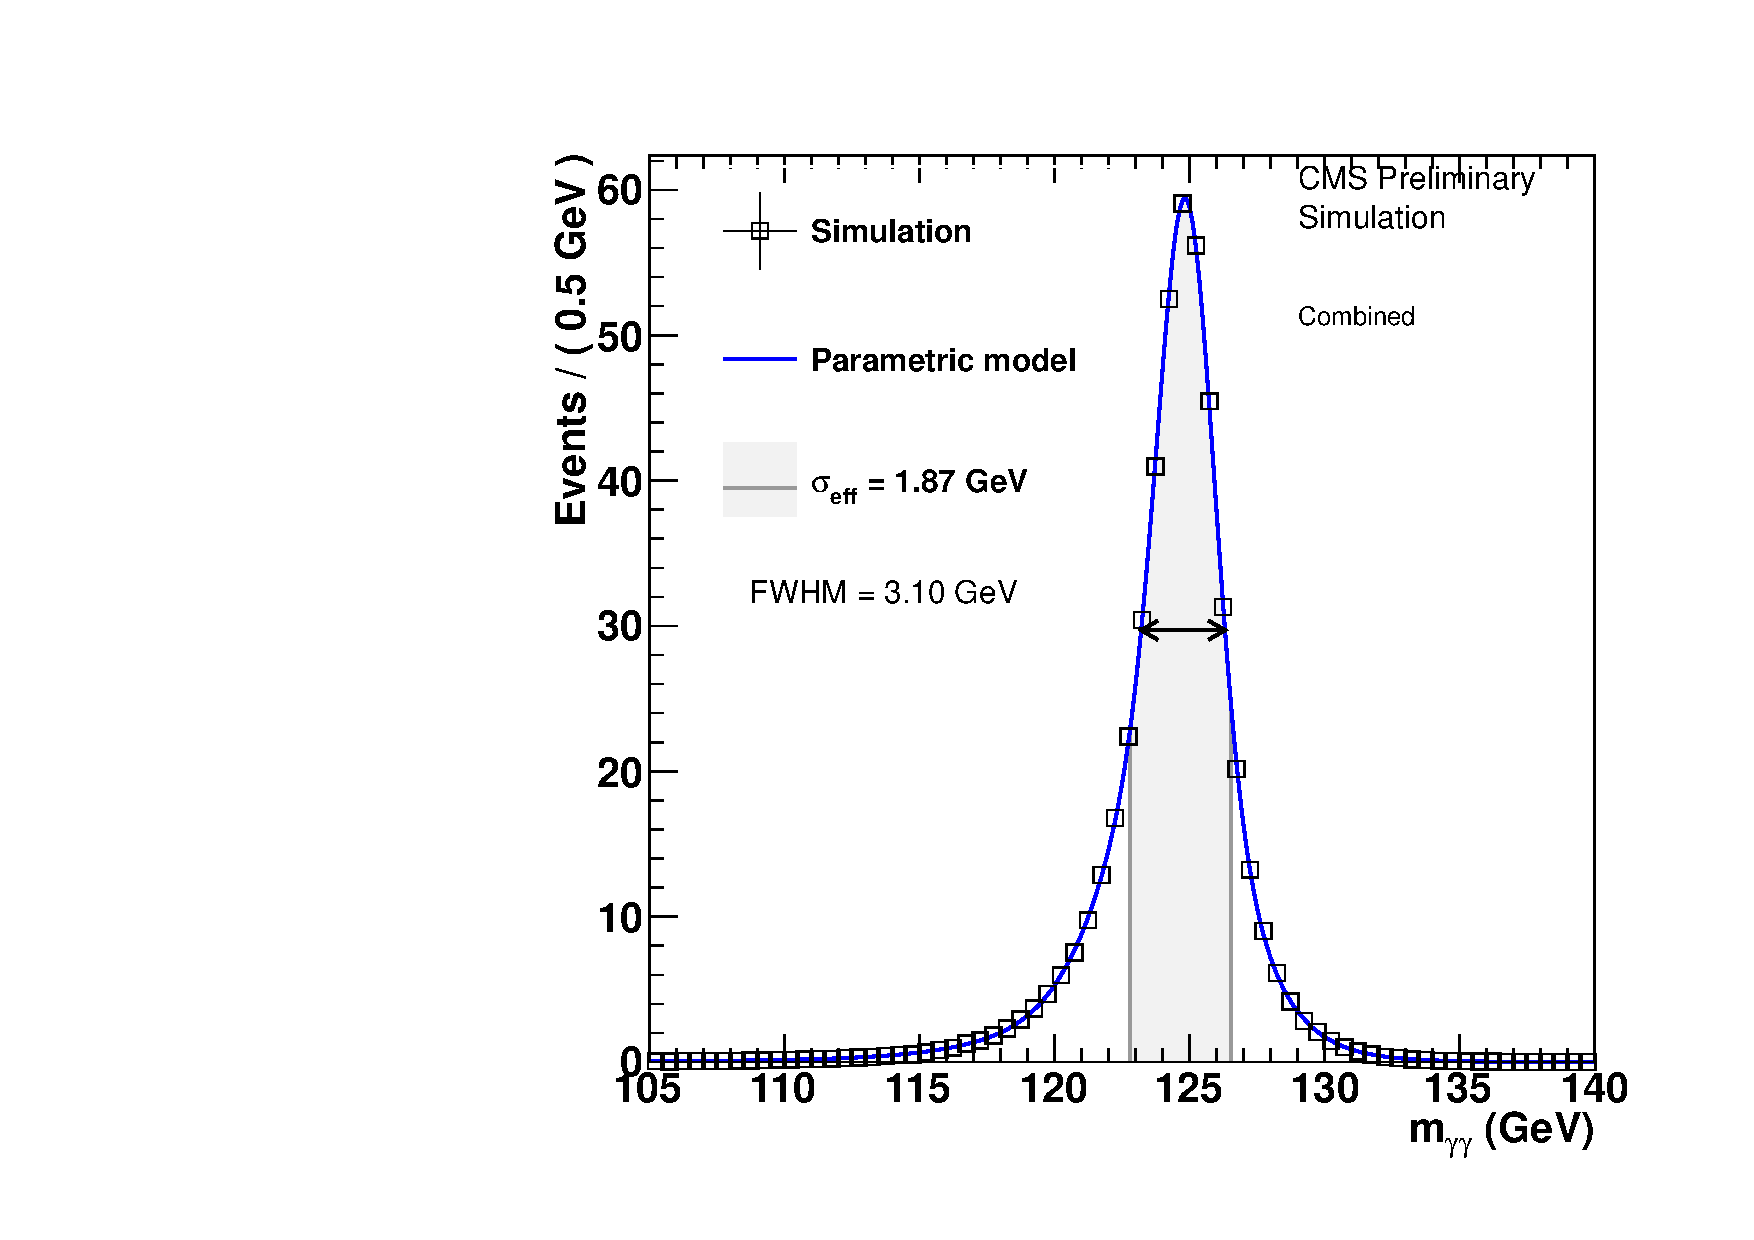
\includegraphics[width=0.49\textwidth]{ch5_anal_and_results/plots/thesis_signal_8TeV/all.pdf}
    \caption{The diphoton invariant mass shape of the \SM signal for the 7~\TeV dataset (left) and 8~\TeV dataset (right). The black square points show the distribution in \MC, where the sum of weights represents the expected number of signal events from a \SM Higgs Boson at 125~\GeV. The blue line shows the shape of the parametric model used to represent the signal.}
    \label{fig:sig_shape}
  \end{center}
\end{figure}

\begin{table}[htbp]
\begin{center}
\caption{Expected number of SM Higgs boson events ($\mH=125\GeV$) and
estimated background (``Bkg.'') at $\mgg=125\GeV$ for all event classes of the 7
and 8\TeV datasets.
The composition of the SM Higgs boson signal in terms of the production
processes and its mass resolution is also given.
Numbers are omitted for production processes contributing less than 0.05\% to the signal.}
\resizebox{\columnwidth}{!}{%%%% ---- beginning of resize
\begin{tabular}{|c|r|r|rrrrr|c|c|r|}
\hline                                                                                                                                          
\multicolumn{2}{|c|}{\multirow{3}{*}{Event classes}} & \multicolumn{8}{c|}{SM Higgs boson expected signal (\mH=125\GeV)} & \multicolumn{1}{c|}{Bkg.} \\
\cline{3-10}
\multicolumn{2}{|c|}{} & \multirow{2}{*}{Total} & \multirow{2}{*}{ggH} & \multirow{2}{*}{VBF} & \multirow{2}{*}{WH} & \multirow{2}{*}{ZH} & \multirow{2}{*}{\ttH} & $\sigma_\mathrm{eff}$ & $\sigma_\mathrm{FW}$ & \multicolumn{1}{c|}{\footnotesize{($\text{GeV}^{-1}$)}} \\
\multicolumn{2}{|c|}{} & & & & & & & \footnotesize{(GeV)} & \footnotesize{(GeV)} &  \\
\hline
\multirow{11}{*}{\begin{sideways}{7\TeV 5.1fb$^{-1}$}\end{sideways}}
& Untagged 0 & 5.8 & 79.8\% & 9.9\% & 6.0\% & 3.5\% & 0.8\% & 1.11 & 0.98 & 11.0 \\ 
& Untagged 1 & 22.7 & 91.9\% & 4.2\% & 2.4\% & 1.3\% & 0.2\% & 1.27 & 1.09 & 69.5 \\ 
& Untagged 2 & 27.1 & 91.9\% & 4.1\% & 2.4\% & 1.4\% & 0.2\% & 1.78 & 1.40 & 134.6 \\ 
& Untagged 3 & 34.1 & 92.1\% & 4.0\% & 2.4\% & 1.3\% & 0.2\% & 2.36 & 2.01 & 311.9 \\ 
\cline{2-11}
& VBF dijet 0 & 1.6 & 19.3\% & 80.1\% & 0.3\% & 0.2\% & 0.1\% & 1.41 & 1.17 & 0.5 \\ 
& VBF dijet 1 & 3.0 & 38.1\% & 59.5\% & 1.2\% & 0.7\% & 0.4\% & 1.65 & 1.32 & 3.5 \\ 
\cline{2-11}
& VH tight $\ell$ & 0.3 & ---~~ & ---~~ & 77.2\% & 20.6\% & 2.2\% & 1.61 & 1.31 & 0.1 \\ 
& VH loose $\ell$ & 0.2 & 3.6\% & 1.1\% & 79.1\% & 15.2\% & 1.0\% & 1.63 & 1.32 & 0.2 \\ 
& VH \MET & 0.3 & 4.5\% & 1.1\% & 41.5\% & 44.6\% & 8.2\% & 1.60 & 1.14 & 0.2 \\ 
& VH dijet & 0.4 & 27.1\% & 2.8\% & 43.7\% & 24.3\% & 2.1\% & 1.54 & 1.24 & 0.5 \\ 
\cline{2-11}
& \ttH tags & 0.2 & 3.1\% & 1.1\% & 2.2\% & 1.3\% & 92.3\% & 1.40 & 1.13 & 0.2 \\ 
\hline
\noalign{\vskip 1mm}
\hline
\multirow{14}{*}{\begin{sideways}{8\TeV 19.7fb$^{-1}$}\end{sideways}}
& Untagged 0 & 6.0 & 75.7\% & 11.9\% & 6.9\% & 3.6\% & 1.9\% & 1.05 & 0.79 & 4.7 \\ 
& Untagged 1 & 50.8 & 85.2\% & 7.9\% & 4.0\% & 2.4\% & 0.6\% & 1.19 & 1.00 & 119.6 \\ 
& Untagged 2 & 117.2 & 91.1\% & 4.7\% & 2.5\% & 1.4\% & 0.3\% & 1.46 & 1.15 & 418.2 \\ 
& Untagged 3 & 153.1 & 91.6\% & 4.4\% & 2.4\% & 1.4\% & 0.3\% & 2.04 & 1.56 & 870.3 \\ 
& Untagged 4 & 121.4 & 93.1\% & 3.6\% & 2.0\% & 1.1\% & 0.2\% & 2.62 & 2.14 & 1401.3 \\ 
\cline{2-11}
& VBF dijet 0 & 4.5 & 17.8\% & 81.8\% & 0.2\% & 0.1\% & 0.1\% & 1.30 & 0.94 & 0.8 \\ 
& VBF dijet 1 & 5.6 & 28.5\% & 70.5\% & 0.6\% & 0.2\% & 0.2\% & 1.43 & 1.07 & 2.7 \\ 
& VBF dijet 2 & 13.7 & 43.8\% & 53.2\% & 1.4\% & 0.8\% & 0.8\% & 1.59 & 1.24 & 22.1 \\ 
\cline{2-11}
& VH tight $\ell$ & 1.4 & 0.2\% & 0.2\% & 76.9\% & 19.0\% & 3.7\% & 1.63 & 1.24 & 0.4 \\ 
& VH loose $\ell$ & 0.9 & 2.6\% & 1.1\% & 77.9\% & 16.8\% & 1.5\% & 1.60 & 1.16 & 1.2 \\ 
& VH \MET & 1.8 & 16.3\% & 2.7\% & 34.4\% & 35.4\% & 11.1\% & 1.68 & 1.17 & 1.3 \\ 
& VH dijet & 1.6 & 30.3\% & 3.1\% & 40.6\% & 23.4\% & 2.6\% & 1.31 & 1.06 & 1.0 \\ 
\cline{2-11}
& \ttH lepton & 0.5 & ---~~ & ---~~ & 1.6\% & 1.6\% & 96.8\% & 1.34 & 1.03 & 0.2 \\ 
& \ttH multijet & 0.6 & 4.1\% & 0.9\% & 0.8\% & 0.9\% & 93.3\% & 1.34 & 1.03 & 0.6 \\ 
\hline
\end{tabular}
}%%%% ---- end of resize

\label{tab:sig_shape}
\end{center} 
\end{table}


                                                                                                             

  
\begin{figure}
  \begin{center}
    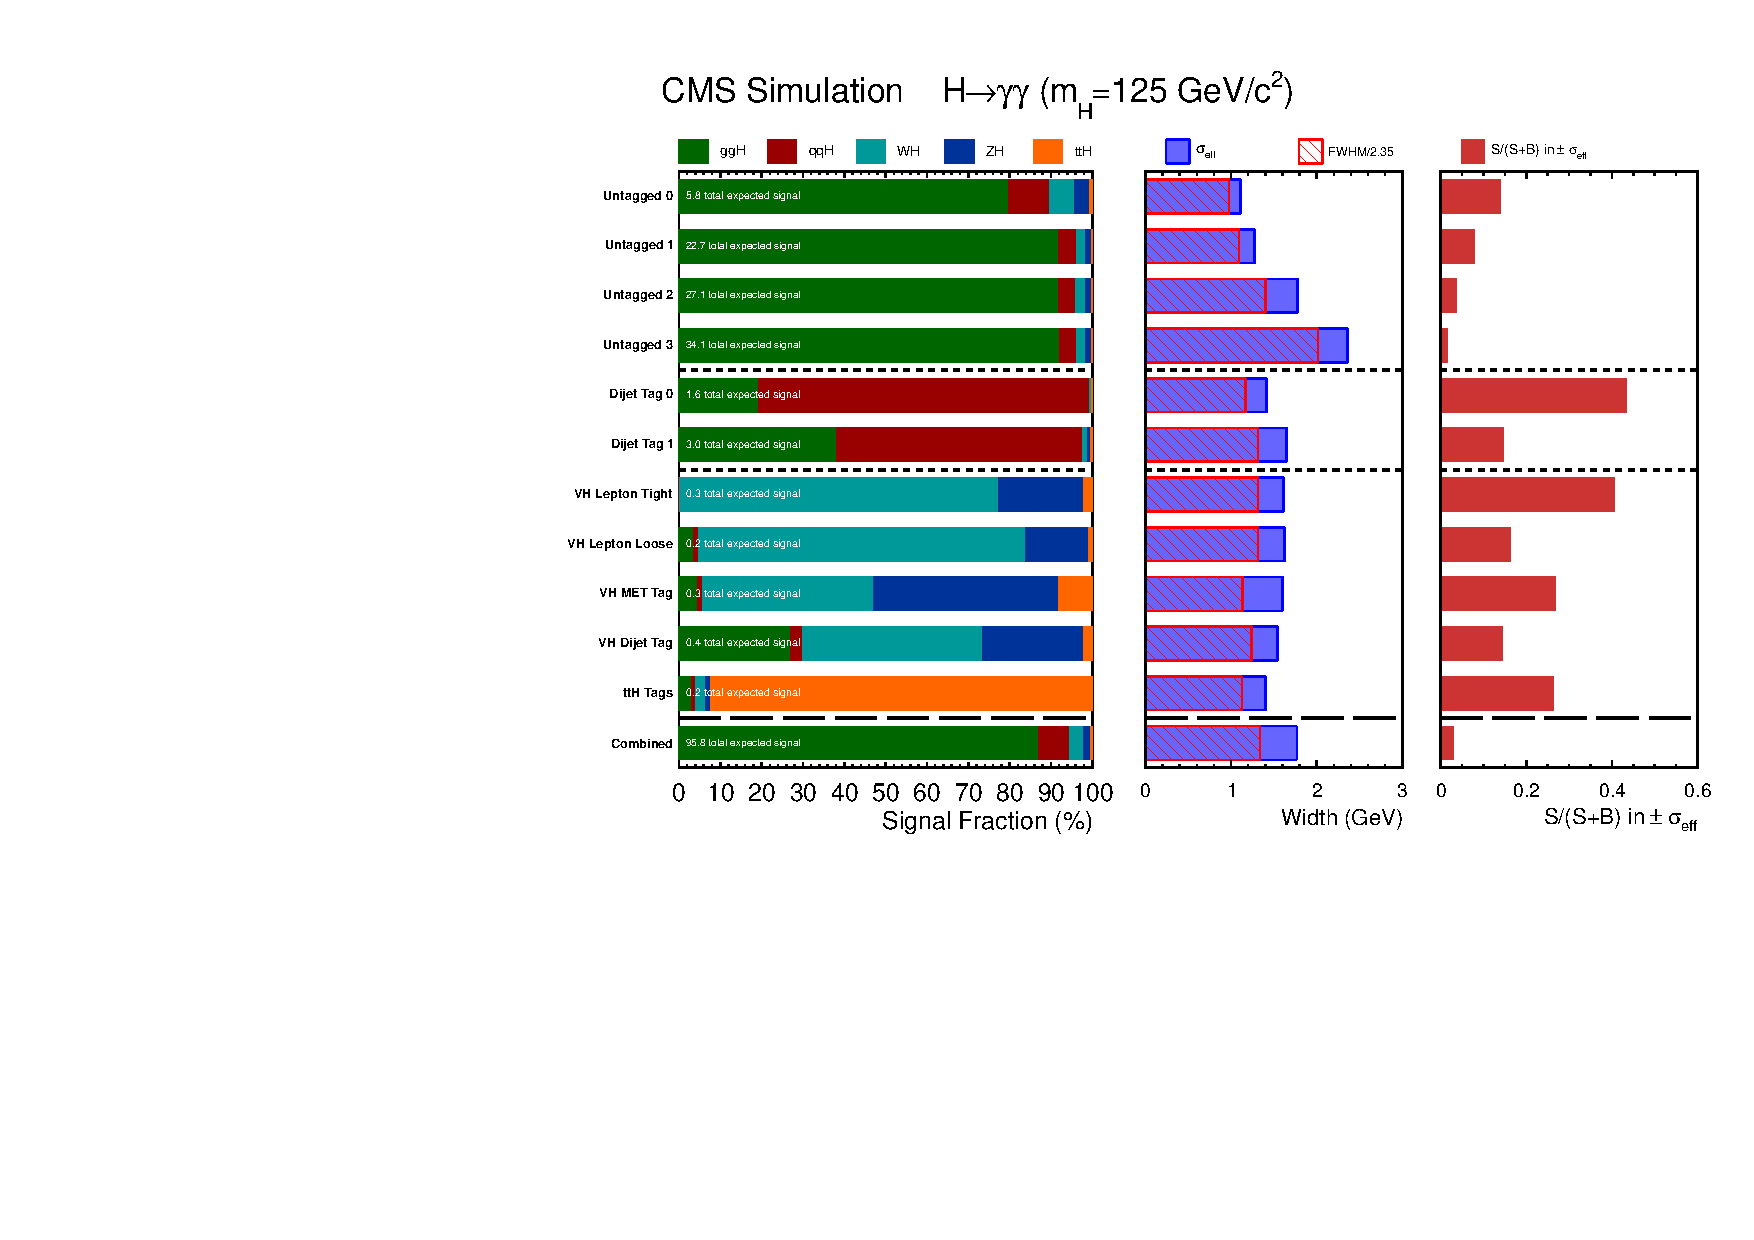
\includegraphics[width=0.99\textwidth]{ch5_anal_and_results/plots/thesis_signal_7TeV/signalComposition.pdf} \\
    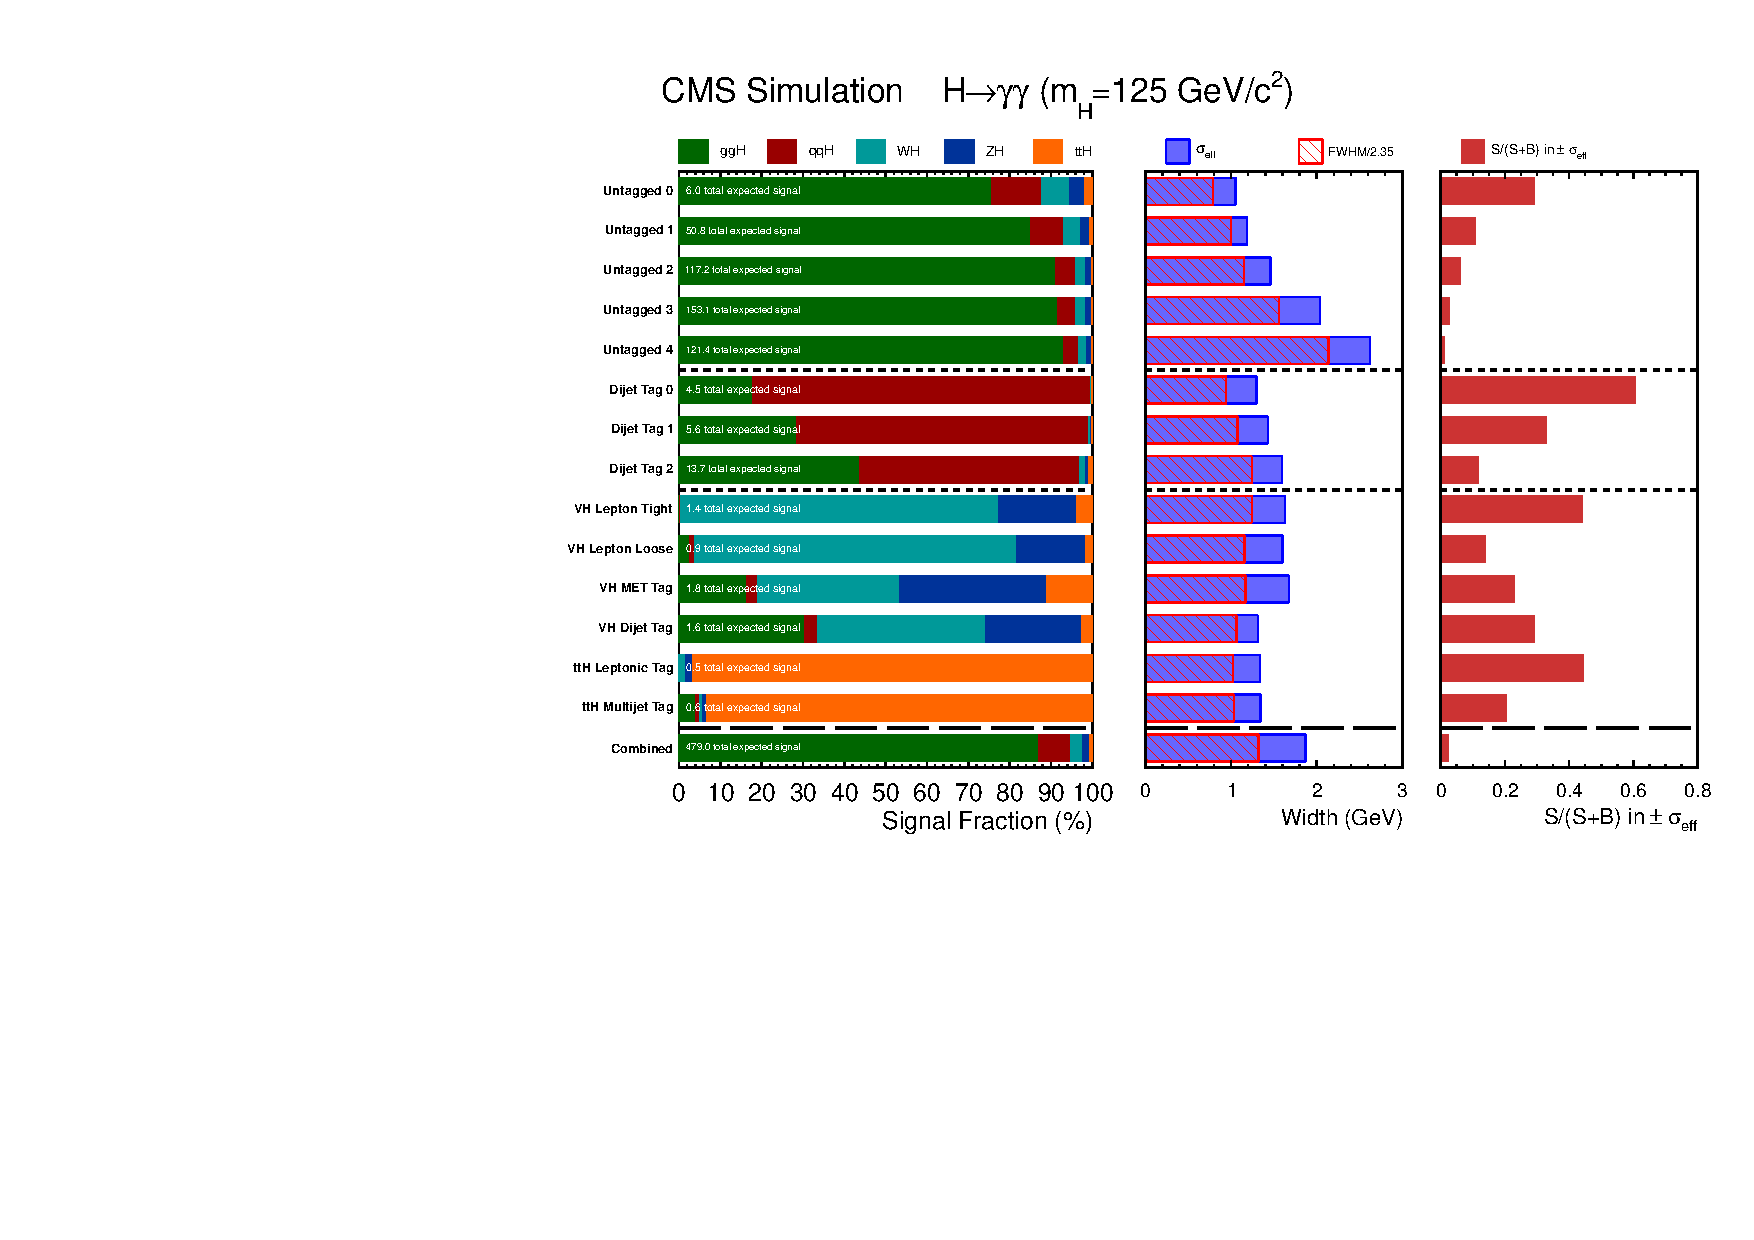
\includegraphics[width=0.99\textwidth]{ch5_anal_and_results/plots/thesis_signal_8TeV/signalComposition.pdf}
    \caption{The expected composition and resolution of the signal for a \SM Higgs at 125~\GeV in the 7~\TeV dataset (top) and 8~\TeV dataset (bottom). The left diagram shows the break down of the signal in each event class by category: \ggH (green), \VBF (red), \WH (turqoise), \ZH (blue), \ttH (orange). The middle shows the expected resolution in each event class in terms of \sigeff and \sigFW. The right diagram shows the expected signal over signal plus background ratio in a window of $\pm\sigeff$ around \mH=125~\GeV.}
    \label{fig:signal_composition}
  \end{center}
\end{figure}
  
\subsection{Sideband analysis}
\label{sec:sig_sideband}

The signal model shape is mapped by the categorisation scheme described in Sec.~\ref{sec:inclusive_cats_sideband} whereby events nearer the signal peak are collected in bins with higher sensitivity (see Fig.~\ref{fig:sideband_cats}). The statistical method used for the sideband method is not a parametric shape analysis like the \MFM but implemented as a simple counting experiment, across the analysis bins, inside the signal region, which is defined as a $\pm$2\% window around the hypothesised Higgs mass, \mH. This is simply the sum of weights of the \MC samples in each analysis bin inside the window for values of \mH for which their exists \MC. The signal shape, i.e.~the signal distribution in the analysis bins, is linearly interpolated for any intermediate values of \mH. As for the \MFM the \SM production mecahnisms are propagated through the analysis separately. The signal normalization at each Higgs mass is calculated in a similar way as for the \MFM in which the \ea is linearly interpolated between the masses at which there are \MC samples and then scaled by cross section, branching ratio and integrated luminosity. 

% ---- SECTION ----
\section{Background modelling}
\label{sec:background_model}

The background is the most significant unknown in this analysis. The size of the background relative to the signal is large and the invariant mass shape of the backgroud is poorly modelled in \MC. It is known to be a smoothly varying and falling spectrum, however various detector effects such as reconstructions, energy resolution and triggering which are imperfectly modelled in the \MC can distort the shape. Furthermore the contribution of fake photons to the background varies as a function of \mgg and this is not well modelled in the theory or detector simulation. One of the main motivations for having the two analyses described here is that they have completely different ways of measuring the background and consequently serve to cross check each other. Both analyses use entirely data driven methods for extracting the background.  

\subsection{Mass factorised analysis}
\label{sec:envelope}

A fairly unique and novel way of estimating the background, given we have no \emph{a priori} of its shape, has been developed specifically for this analysis. The method, laterly referred to as the ``envelope" method, attempts to parametrise our ignorance of the background shape in a similar way to what is done for normal nuisance parameters when using the negative log likelihood to obtain the best fit value of a quantity and its error using frequentist statistical methods~\cite{FredJames}. To explain better the method let us first consider the simplified case of fitting a probability distribution to a dataset where the probability distribution contains one physical parameter of interest, $x$, (which could for example represent the signal mass) and one nuisance parameter, $\theta$, (which could represent the energy scale uncertainty). In this case we can calculate twice the negative log likelihood, \NLL, at different values of $x$ whilst at each point minmising the likelihood with respect to \theta. 
This would give us the best fit value of $x$ and its error given the variation allowed by \theta. This is represented in Fig.~\ref{fig:envelope_explain1} by the solid black line. The best fit value of $x$ is given at the minimum of the likelihood and the 1$\sigma$ error interval defined as the range where \NLL$\leq1$. This is known as the ``profile likelihood method" as the nuisance parameter, $\theta$, is ``profiled" in the fit. In other words, for a given value of $x$ the value of $\theta$ which minimizes the likelihood is chosen. One can redo the likelihood scan fixing $\theta$ to its value at the best fit and this gives a narrower likelihood curve, demonstrated by the solid blue line in Fig.~\ref{fig:envelope_explain1}. In this case the error, the range for which \NLL$\leq1$, is smaller as one would expect given the nuisance parameter is now frozen. This is equivalent to the statistical error only, as the systematic component parametrised by $\theta$ is ignored. One can now also build up a multitude of curves by setting the nuisance parameter $\theta$ to arbitary values and rescanning the likelihood, these are shown in Fig.~\ref{fig:envelope_explain1} as the red dashed lines. It should be clear that by taking the ``envelope" around the potentially infinite set of red curves one can reproduce the black line representing the full profile fit providing the full $\theta$ phase space is sampled enough times. 
This is shown in the figure by the magenta line which becomes smoother as more sets of $\theta$ values are chosen. It is worth noting that not all of the red curves (of which there are infinitely many) necessarily have to touch the black line: a very extreme value of $\theta$ will give a bad fit and the corresponding red dashed curve would be off the plot. In this way one could in principal ``reverse-engineer" the profile likelihood method such that the profiling of the nuisance parameter $\theta$ is not done as a continuous minimisation but as a series of discrete minimisations, where the minimum \NLL for a given value of $x$ is taken as the minimum \NLL for this $x$ and all discrete choices of $\theta$ that have been chosen. Clearly, for a case in which the nuisance parameter $\theta$ is continous this is inefficient and unnecessary but it is effective if the nuisance parameter can only take discrete values.

\begin{figure}
\begin{center}
  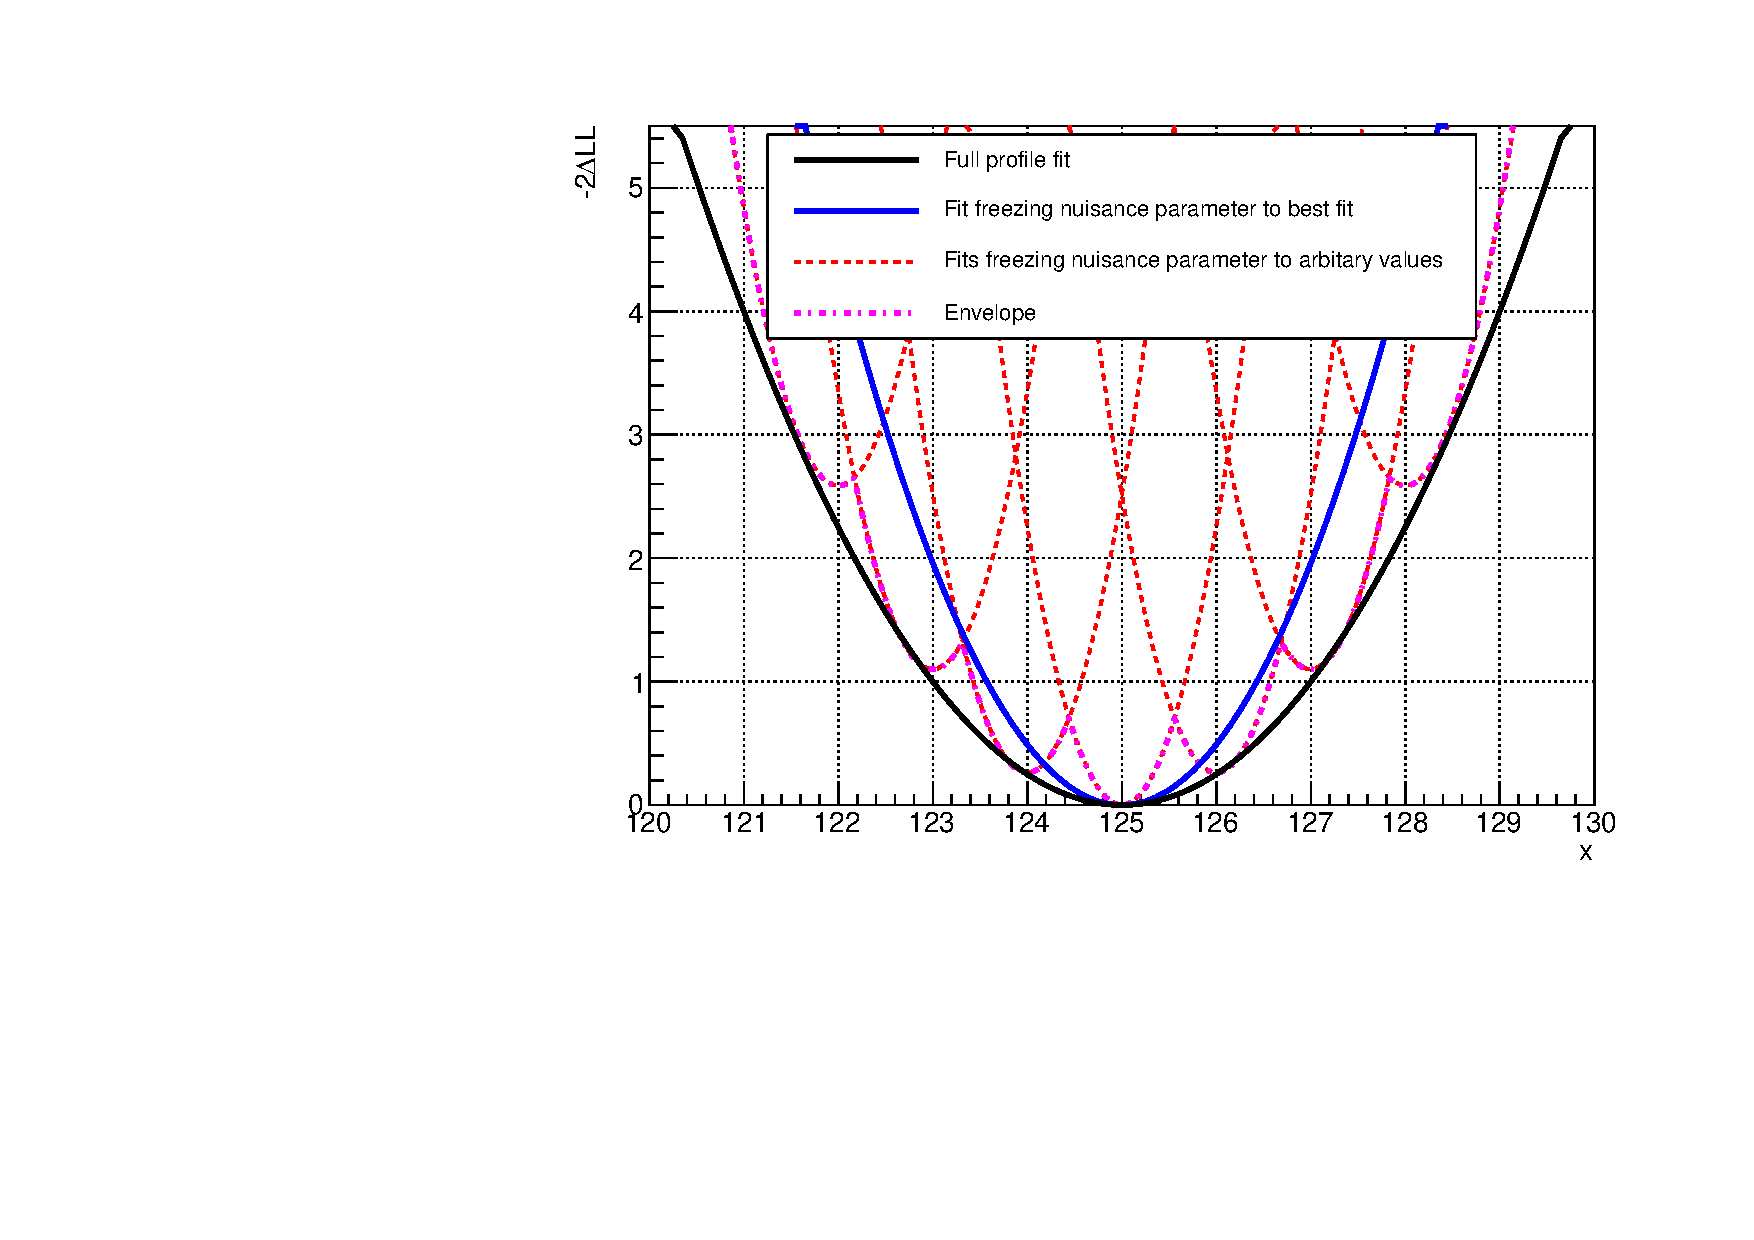
\includegraphics[width=0.8\textwidth]{ch5_anal_and_results/plots/envelope_explain.pdf}
  \caption{A demonstration of the method of ``profiling the likelihood". Here the \NLL is scanned as a function of a physical parameter of interest $x$ with a nuisance parameter $\theta$ in three cases: 1) where $\theta$ is freely floating (black line), 2) where $\theta$ is set to its value at the \NLL minimum (blue line), 3) for several arbitary choices of $\theta$ (red line).}
  \label{fig:envelope_explain1}
\end{center}
\end{figure}

In this analysis the background parametrisation is entirely unknown. So in principle if we could sample the infinite phase space of possible function choices we could use the method just described to profile the choice. In this way we find the function that minimises the likelihood for any given value of the parameter of interest $x$. This will then pick the function which fits the data best (minimises the likelihood) and can enlarge the error.
Lets now consider a simplified case of the real situation. Imagine we have a large steeply falling background which can be parametrised by two possible choices: a single term power law, $x^{-p}$, and a single term exponential, $e^{-px}$. We have a small Gaussian like signal component and our \POI is the size of this single, $\mu$. The best fit distributions are shown for a generated pseduo-dataset in the left hand plot of Fig.~\ref{fig:envelope_explain2}. The right hand plot of Fig.~\ref{fig:envelope_explain2} shows the likelihood scan across the parameter $\mu$, which represents the size of the signal, for the two chosen functions, the envelope is shown as the green dashed line. One can see that the global best fit is at a value of $\mu=2.83$ with the power law function. The $1\sigma$ error (the point where the \NLL crosses 1) is unchanged with respect to the result using the power law function alone. The $2\sigma$ error (the point where the \NLL crosses 4) however is increase with respect to the result using the power law funciton alone. This is the principal behind the ``envelope" background method. One can see that it is analagous to using a normal nuisance parameter which can only take discrete values. In this case the discrete values index which function is chosen. It means that a specific function choice never has to be made and the error on a given value will increase to account for situations where two or more functions give a similarly good fit. However, there is one more important feature of the method which must be discussed before it can be applied to the data.

\begin{figure}
  \begin{center}
    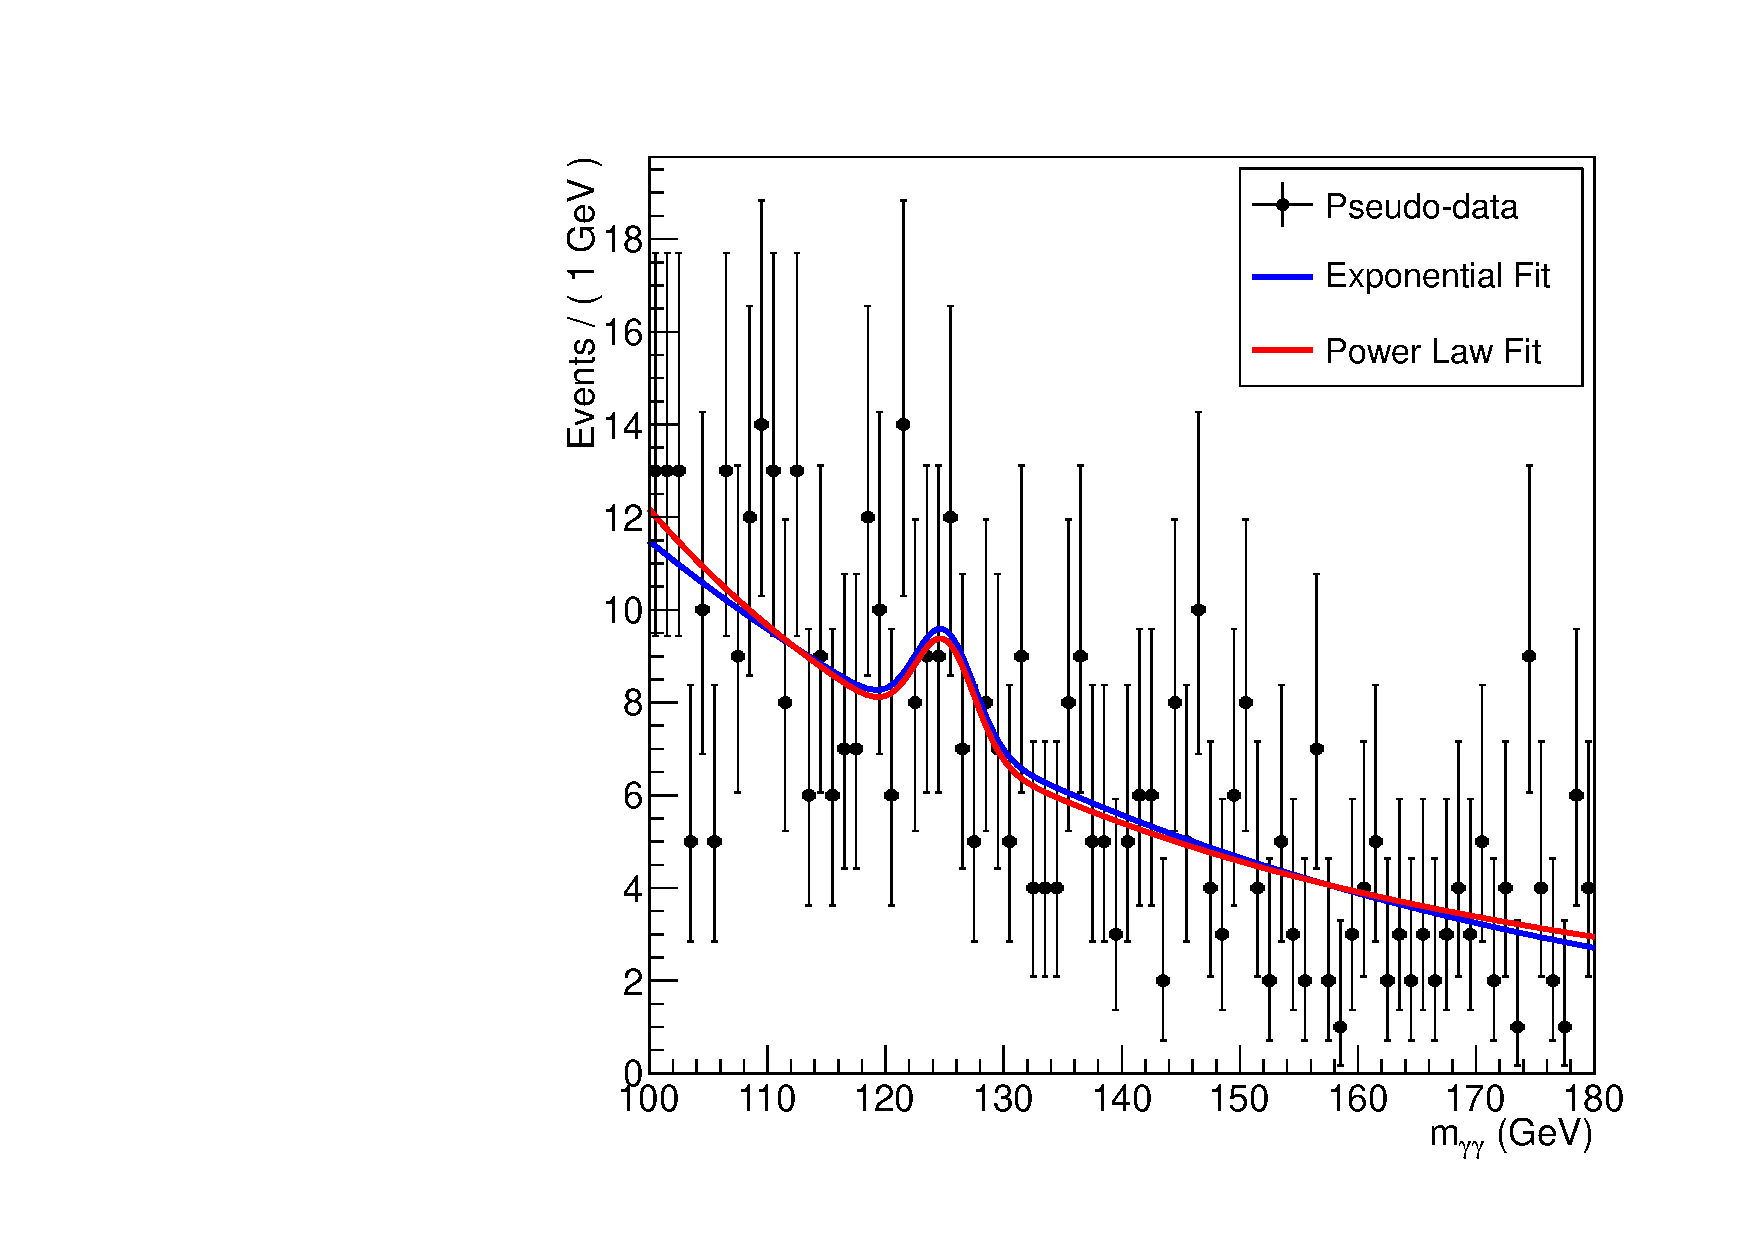
\includegraphics[width=0.49\textwidth]{ch5_anal_and_results/plots/envelope_explain2.pdf}
    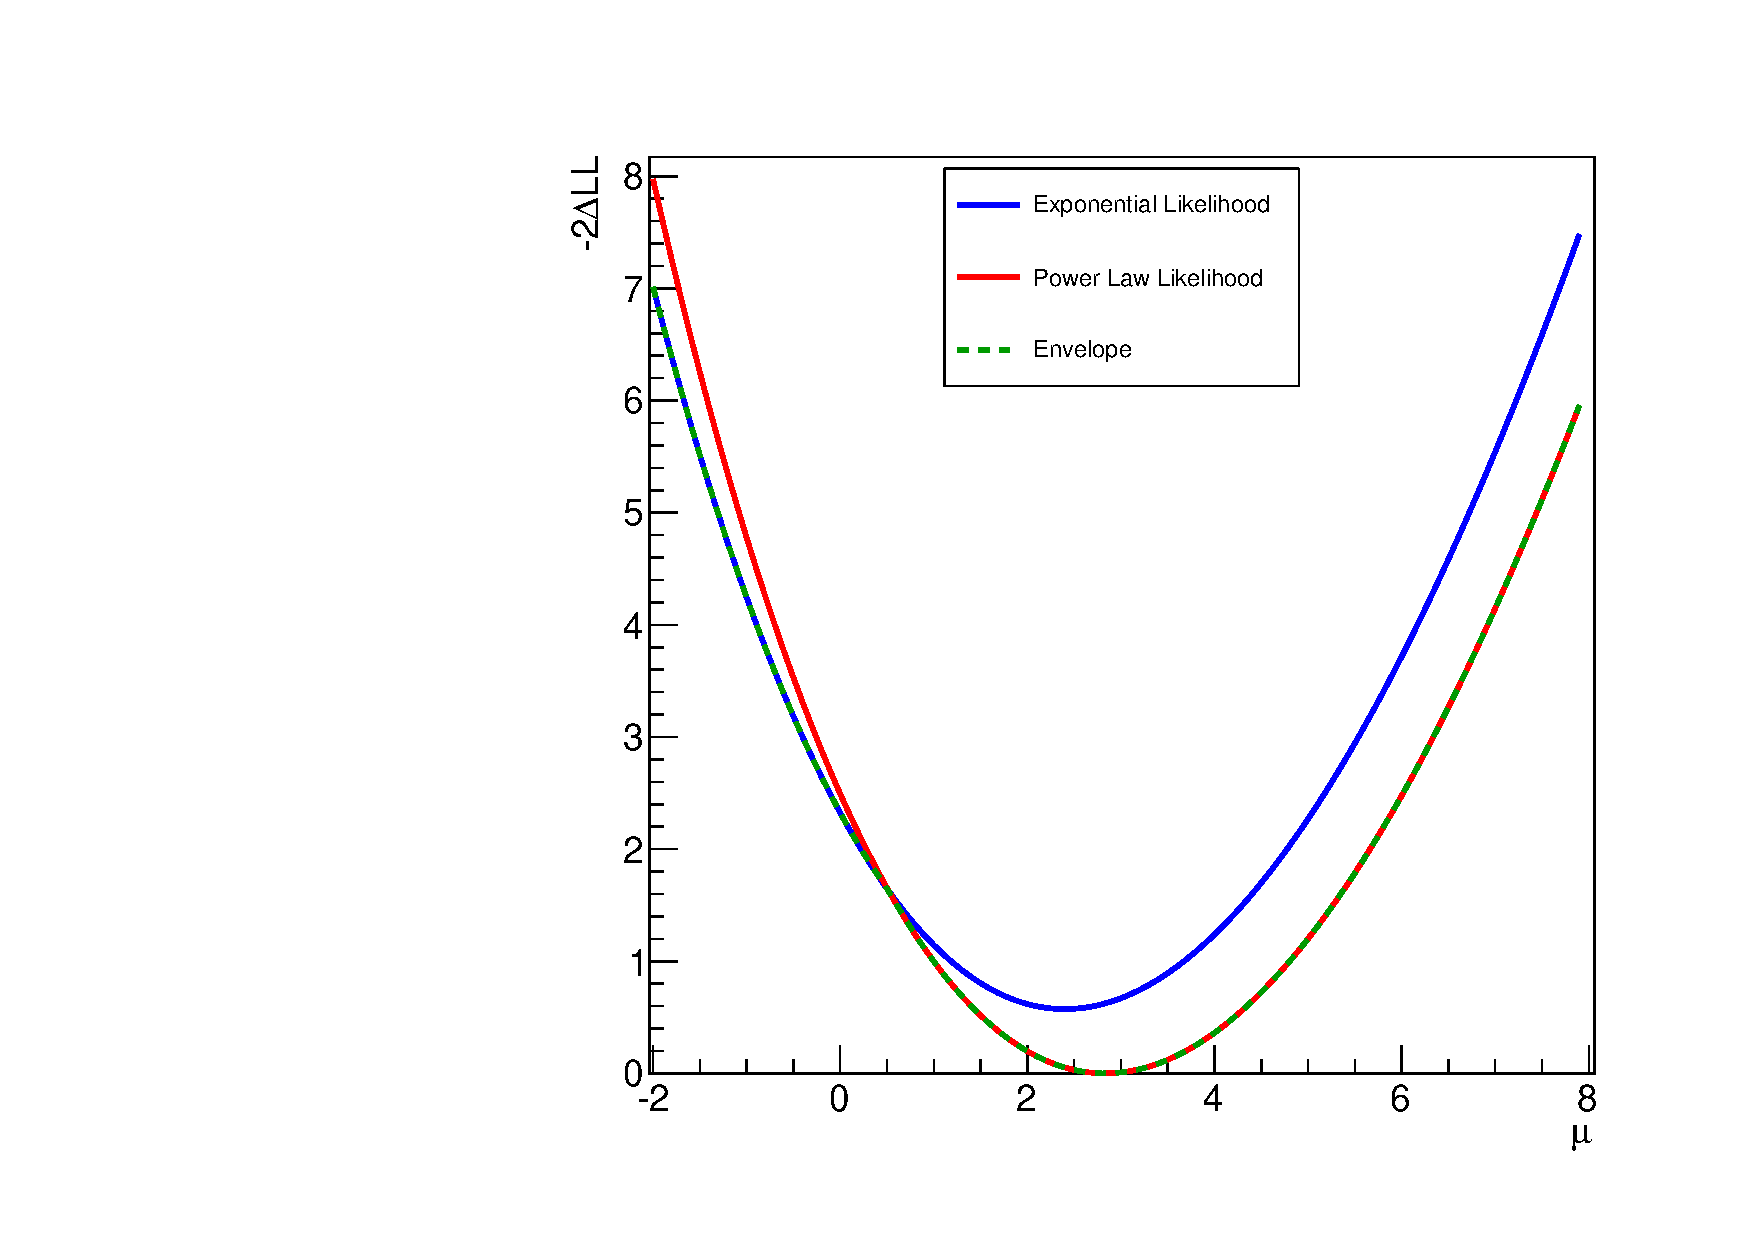
\includegraphics[width=0.49\textwidth]{ch5_anal_and_results/plots/envelope_explain3.pdf}
    \caption{An example of using the envelope in a realistic situation. The plot on the left shows a signal plus background fit to some pseudo-data using two different background function choices; a single term power law (red) and a single term exponential (blue). The plot on the right shows the profile likelihood curve for the signal size, $\mu$, for the two different function choices, where the global minimum is where $\mu=2.83$ and the power law is used as the background choice. The envelope likelihood curve, profiling over the function choices is shows as the green dashed line.}
    \label{fig:envelope_explain2}
  \end{center}
\end{figure}

The concept of the ``envelope" method has now been demonstrated with a simplified example in which two function choices were profiled and both these functions had one free parameter. However we would like to be able to sample as much of the function phase space possible (i.e.~as many functions as we can) which means there will be choices with different numbers of free parameters. Two functions of the same type but of a different order may give a very similar fit result but the function with more degrees freedom will give a lower negative likelihood value. For example consider the functions $E_{1} = e^{-p_{1}x}$ and $E_{2} = f_{1}e^{-p_{1}x}+(1-f_{1})e^{-p_{2}x}$, which are first and second order exponential sums and have one and three free parameters respectively, not including an overall normalisation term. There may be a case where these give an identical fit (as $f_{1}\to 1$ or $p_{1}\to p_{2}$) however the negative log likelihood will always be lower for a higher parameter fit and therefore the higher order function would always be the minimum of the envelope, at least at the best fit point. This means that for any embedded class of functions, the function which gives the global minimum of the likelihood will be of the highest order allowed. Consequently, a correction scheme has been devised to avoid this problem and to penalise functions in the envelope which have more free parameters but don't necessarily fit the data any better.

The negative log likelihood gets redefined as,

\begin{equation}
  \NLL = -2\ln(\mathcal{L}) + cN_{p},
\end{equation}

where $N_{p}$ is the number of free parameters in the function and $c$ is a constant correction term. Two correction schemes were studid, for values of $c=1$ and $c=2$. The motivation for choosing $c=2$ is an application of the Akaike information criterion, described in Ref.~\cite{akaike}, which states that for large sample sizes the corrected likelihood is,

\begin{equation}
  A = -2\ln(\mathcal{L}) + 2N_{p}.
\end{equation}

It can be seen that the correction term here is $2N_{p}$, which gives a value of $c=2$, in others words a correction of 2 per free parameter. 

The argument for using a correction of $c=1$ is a little more natural and arises from the assumption that in the high statistics limit for a binned dataset, $\NLL\approx\chi^{2}$. Given a value of the $\chi^{2}$ one can calculate the $\chi^{2}$ $p$-value given the number of degrees of freedom, $N$, which is equal to the number of bins, $b$, minus the number of free parameters in the fit function, $N_{p}$, thus the $p$-value can be expressed as $p(\chi^{2},b-N_{p})$. One can then determine a new chi squared value, $\chi^{\prime 2}$, defined as the one which would give the equivalent $p$-value but with a different number of degrees of freedom, namely the one in which there are no free parameters in the fit, $p(\chi^{\prime 2},b)$ . It can be seen that there is now an expression for $\chi^{\prime 2}$, which is approximately equivalent to \NLL, which is independet of the number of fit parameters, $N_{p}$, and thus the corrected likelihood is given by,

\begin{equation}
  \NLL = -2\ln(\mathcal{L}) + \chi^{\prime 2} - \chi^{2}.
\end{equation}

The correction term, $\chi^{\prime 2} -\chi^{2}$, depends on the number of bins, the number of free fit parameters and the quality of the original fit (the $\chi^{2}$ $p$-value). Figure~\ref{fig:envelope_chi2_correction} shows how the size of the correction varies for functions with different numbers of fit parameters. It can be seen that on average the correction is given by,

\begin{equation}
  \chi^{\prime 2} - \chi^{2} \approx N_{p}.
\end{equation}

\begin{figure}
  \begin{center}
    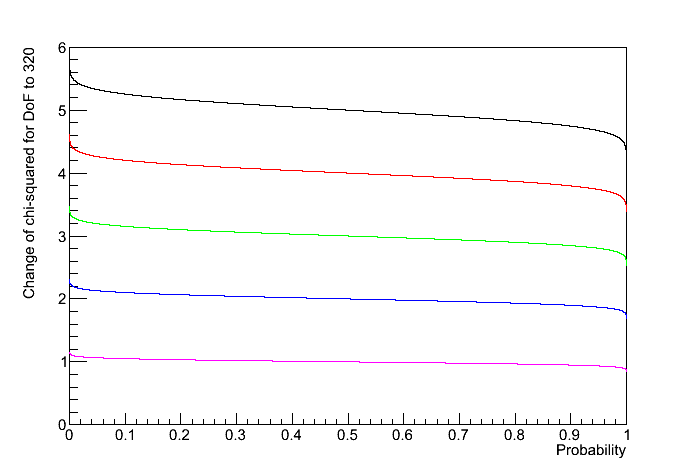
\includegraphics[width=0.49\textwidth]{ch5_anal_and_results/plots/ChisqConv1.png}
    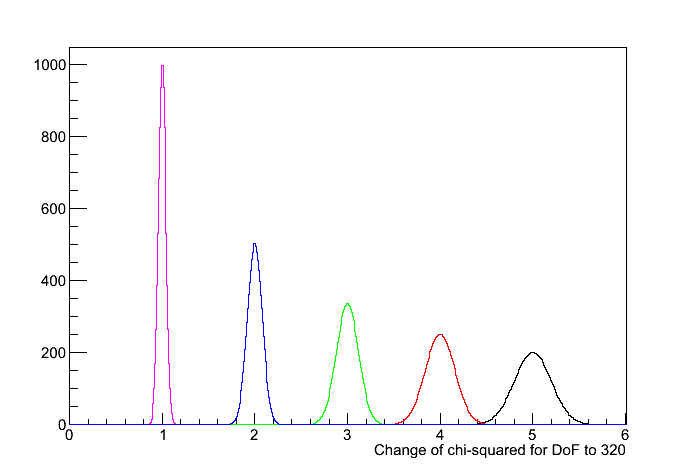
\includegraphics[width=0.49\textwidth]{ch5_anal_and_results/plots/ChisqConv2.png}
    \caption{The value of the correction, $\chi^{\prime 2} - \chi^{2}$, as a function of the fit $p$-value for a fit with 320 bins is shown on the left. The projection of the correction integrated uniformaly over $p$-values is shown on the right. The five different coloured lines represented fit function with different numbers of free parameters, ranging from one free parameter (pink) up to five free parameters (black).}
    \label{fig:envelope_chi2_correction}
  \end{center}
\end{figure}

The correction scheme used in the analysis was chosen to be $c=1$. This was decided using empirical results of studying the impact on the bias and error coverage on fitting physical parameters when using the envelope method with either correction scheme. Before we cover the results and conclusions of this study, lets first discuss how one decides which functions to include in the envelope.

In principal it would be beneficial to choose any and every function one can think of that can reasonably describe a falling spectrum. In practise this is unfeasible as the combinatorics of the problem rapidly spiral out of control. If an analysis has multiple categories, $N_{c}$, and one chooses multiple background functions in each category, $N_{f}$, then the number of combinations goes like $N_{f}^{N_{c}}$ which rapidly makes the problem computationally impossible. Instead, one has to choose a smaller number of functions which reasonably cover the phase space of infinite functions. The functions used in this analysis come in four main classes. They are as follows (note an overall normalisation term is not included in the equations below),

\begin{itemize}
  \item \textit{Exponential recursive sum} - a sum of terms like $e^{-px}$.
    \begin{equation}
      p(x) = c_{1}e^{-p_{1}x} + (1-c_{1})c_{2}e^{-p_{2}x} + (1-c_{2})c_{3}e^{-p_{3}x} + ... + (1-c_{n-1})e^{-p_{n}x}
    \end{equation}
    \begin{itemize}
      \item This has $2n-1$ free parameters per order. The functions are labelled by the number of free parameters so the lowest order is \texttt{exp1} then \texttt{exp3}, \texttt{exp5} and so on.
    \end{itemize}

  \item \textit{Power law recursive sum} - a sum of terms like $x^{-p}$.
    \begin{equation}
      p(x) = c_{1}x^{-p_{1}} + (1-c_{1})c_{2}x^{-p_{2}} + (1-c_{2})c_{3}x^{-p_{3}} + ... + (1-c_{n-1})x^{-p_{n}}
    \end{equation}
    \begin{itemize}
      \item This has $2n-1$ free parameters per order. The functions are labelled by the number of free parameters so the lowest order is \texttt{pow1} then \texttt{pow3}, \texttt{pow5} and so on.
    \end{itemize}

  \item \textit{Laurent series} - The best fit value for a single order power term is around -4.3. Consequently the laurent series is a sum of terms like $x^{-n}$ expanded around $x^{-4}$.
    \begin{equation}
      p(x) = c_{1}x^{-4} + (1-c_{1})c_{2}x^{-5} + (1-c_{2})c_{3}x^{-3} + (1-c_{3})c_{4}x^{-6} + ...
    \end{equation}
    \begin{itemize}
      \item This has $n-1$ free parameters per order. The functions are labelled by the number of free parameters so the lowest order is \texttt{lau1} then \texttt{lau2}, \texttt{lau3} and so on.
    \end{itemize}

  \item \textit{Bernstein polynomials} - These are polynomials in the Bernstein basis~\cite{bernsteins1,bernsteins2}. A Bernstein polynomial of degree $n$ is given by,
  \begin{equation}
    p(x) = \displaystyle\sum_{1}^{n}p_{i}\frac{n!}{i!(n-i)!}x^{i}(1-x)^{n-i}
  \end{equation}
  \begin{itemize}
    \item This has $n$ free parameters per order. The functins are labelled by the number of free parameters so the lowest order is \texttt{pol1} then \texttt{pol2}, \texttt{pol3} and so on.
  \end{itemize}
\end{itemize}

One then has to determine which order functions of each of these classes is used in the envelope for a given dataset. To pick the lowest order used a simple goodness of fit test is used and has the loose requirement that the $\chi^{2}$ $p$-value of the fit is greater than 0.01. To pick the higest order used in the envelope an $f$-test style requirement is imposed~\cite{ftest}. If two functions of the same class have $n$ and $n+m$ free parameters respectively then, in the high statistics limit, the difference in \NLL between the two functions is distributed as $\chi^{2}$ with $m$ degrees of freedom. Consequently the difference in \NLL between the two fits is converted into a $\chi^{2}$ $p$-value and the next higher order function is included if $p<0.1$. In other words if the higher order function does not improve the fit it is not included. This determines which functions are included in the envelope for each category and ranges anywhere between 4 and 9.

In order to assess the bias and coverage properties of the envelope method a few functions are chosen as ``truth" models from which to generate pseudo-data and test the statistical validity of the method. A single function of each class is chosen and the order determined by the same $f$-test but with a tighter requirement that $p<0.05$. These models are first fit to the data and then the pseduo-data generated from these values. The comparison of the systematic bias to statistical uncertainty is determined by the pull distribution,

\begin{equation}
  pull(\mu) = \frac{\mu_{fit} - \mu_{inj}}{\sigma_{fit}},
\end{equation}

where $\mu_{inj}$ is the injected signal strength in the toy, $\mu_{fit}$ is the fitted signal strength and $\sigma_{fit}$ is the error on the fitted signal strength. The systematic bias to statistical comparison is then the deviation of the mean of the distribution from zero as compared to the width of this distribution. An unbiased method will give a mean close to 0 and a method which covers accurately will give a width less than or equal to 1.

When using a correction factor of $c=1$, the systematic bias on the signal strength is less than 14\% of the statistical error from the fit and the coverage is accurate for 0.5, 1, 2 and 3$\sigma$ (all the points tested). This was found to be true when generating toy experiments for a range of different signal strengths and for signal at different mass values. The bias and coverage have also been tested when removing the ``truth" model from the set of envelope functions, when removing all functions of the same class as the ``truth" model and when using various convulted truth models such as a histogram spline of the data, a kernel density estimator (sum of Gaussians)~\cite{kde} and a hybrid of different functions patched together. All of these cases also demonstrated a reasonable level of bias and coverage. 

When using a correction factor of $c=2$ the systemastic bias is larger than this, in extreme cases it can reach 30\% of the statistical uncertainty and in these cases it is common that the method undercovers especially at higher values of $\sigma$. Consequently, for this analysis a correction factor of $c=1$ is chosen. The tests described above to ascertain the statistical validity of the method are performed for each individual category of the analysis and furthermore for the categories combined together in years and the whole ensemble of categories. The method has sensible behaviour in all of these cases.

The invariant mass distributions with the different envelope functions for each of the analysis categories are shown in Figures~\cref{fig:multipdf1,fig:multipdf2,fig:multipdf3,fig:multipdf4,fig:multipdf5,fig:multipdf6}.

\begin{figure}
  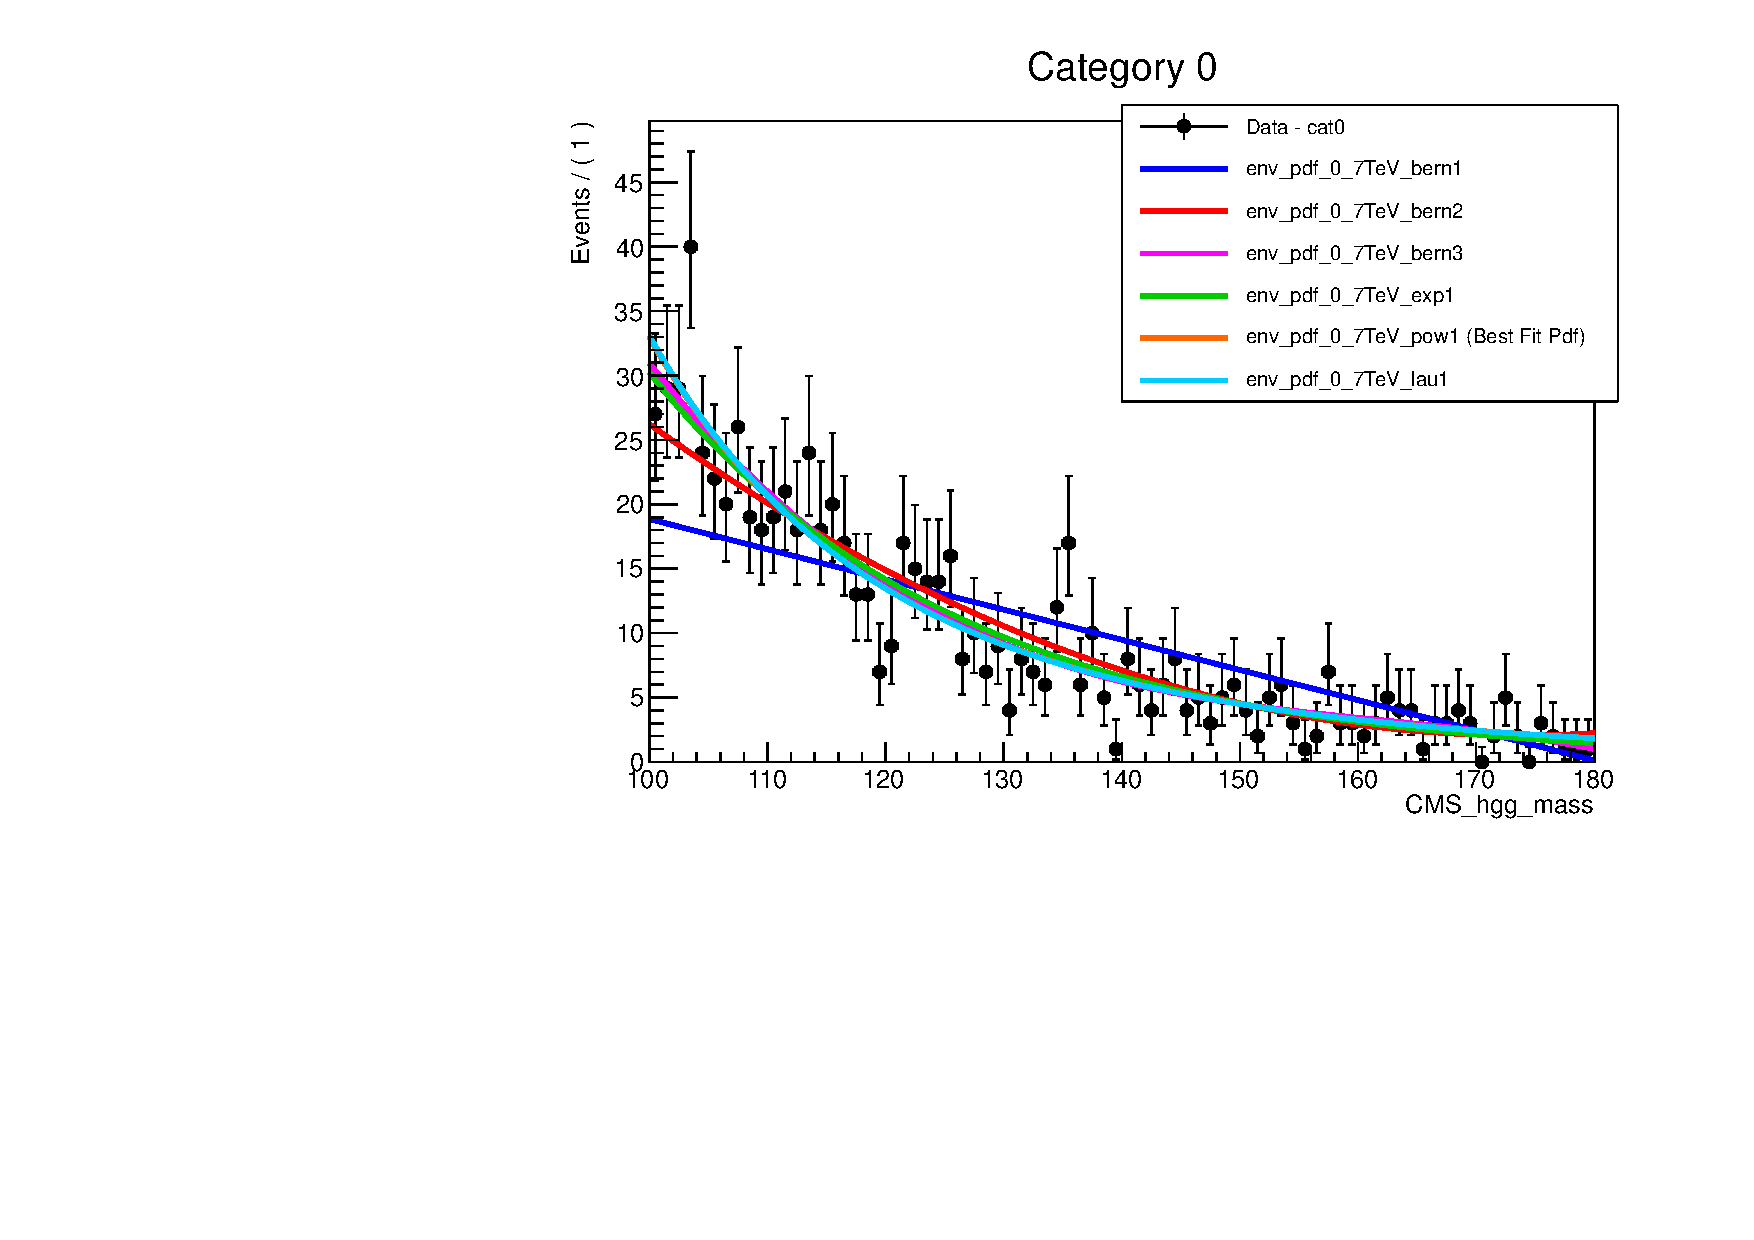
\includegraphics[width=0.49\textwidth]{ch5_anal_and_results/plots/mva_7TeV/multipdf_cat0.pdf}
  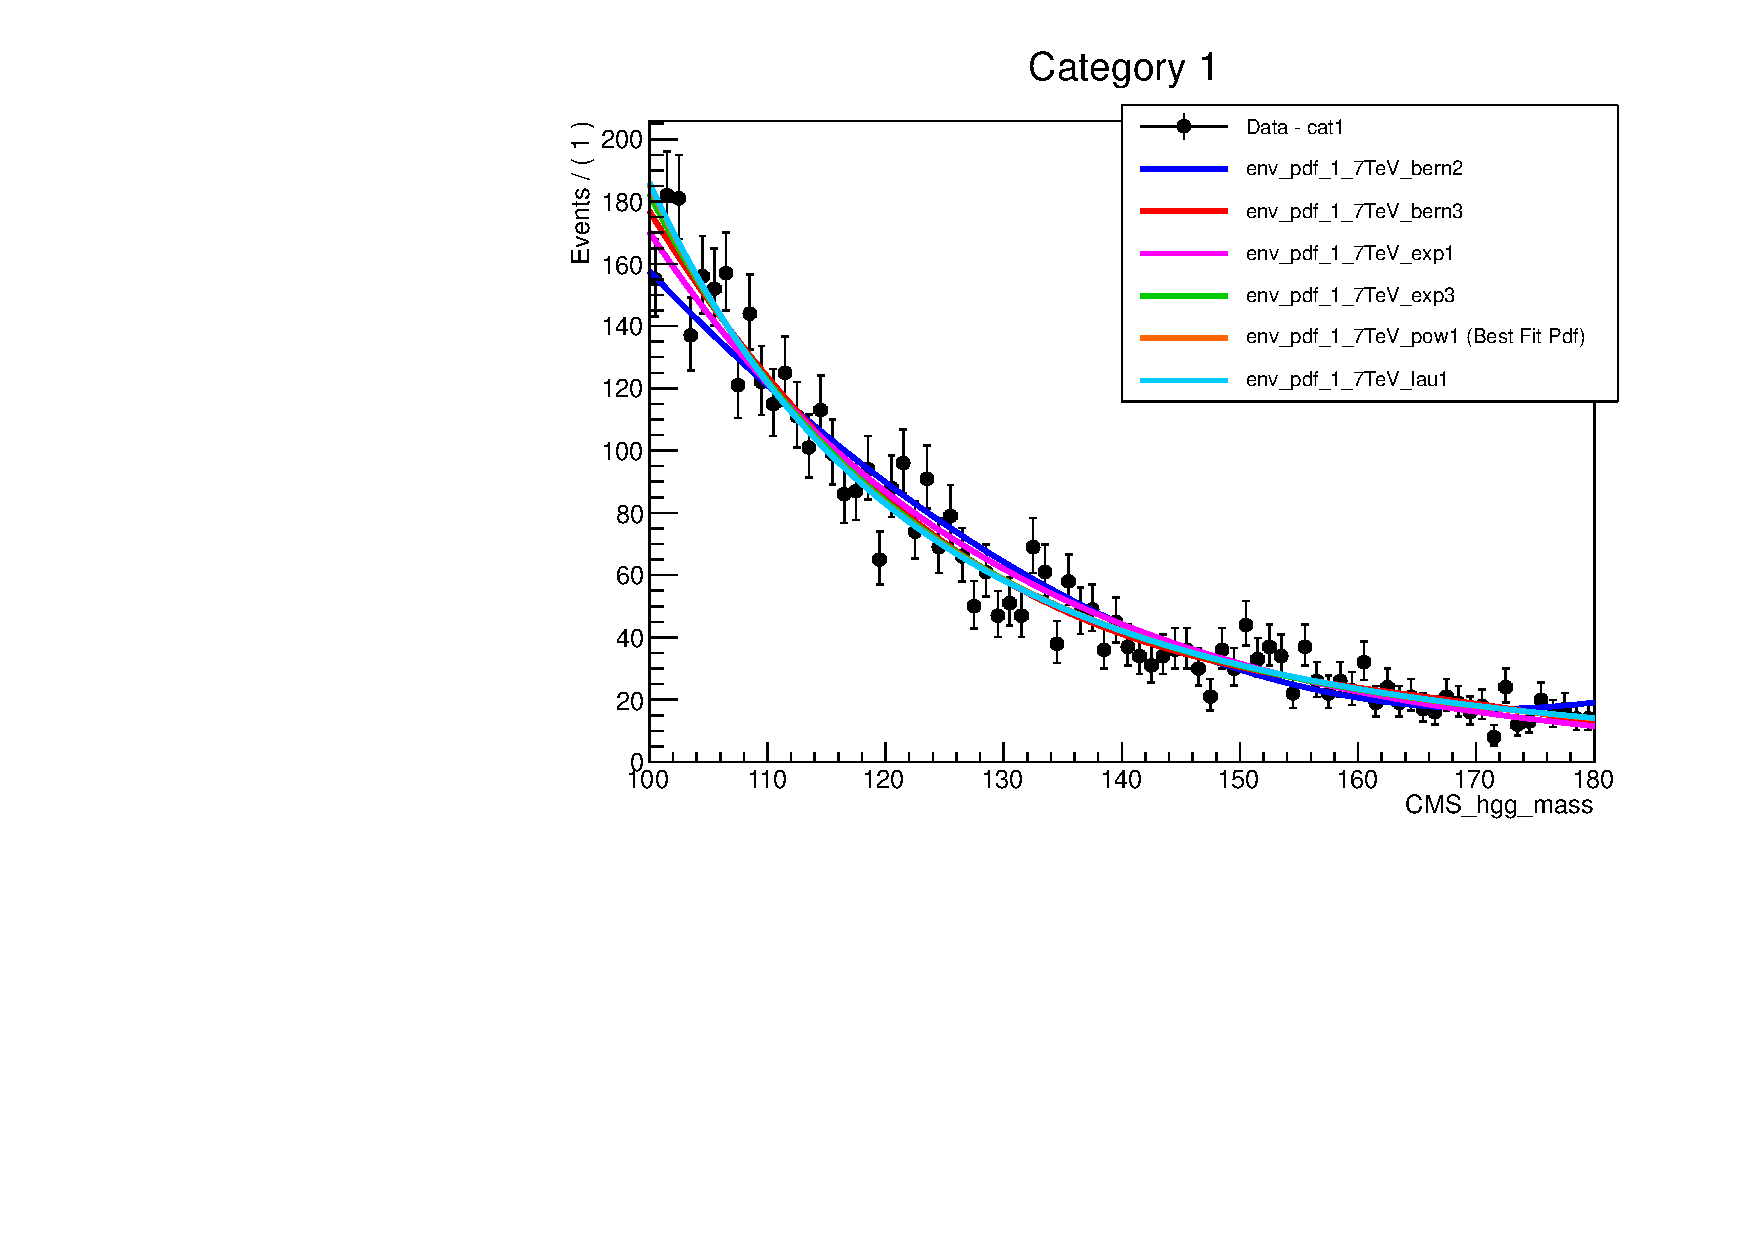
\includegraphics[width=0.49\textwidth]{ch5_anal_and_results/plots/mva_7TeV/multipdf_cat1.pdf}\\
  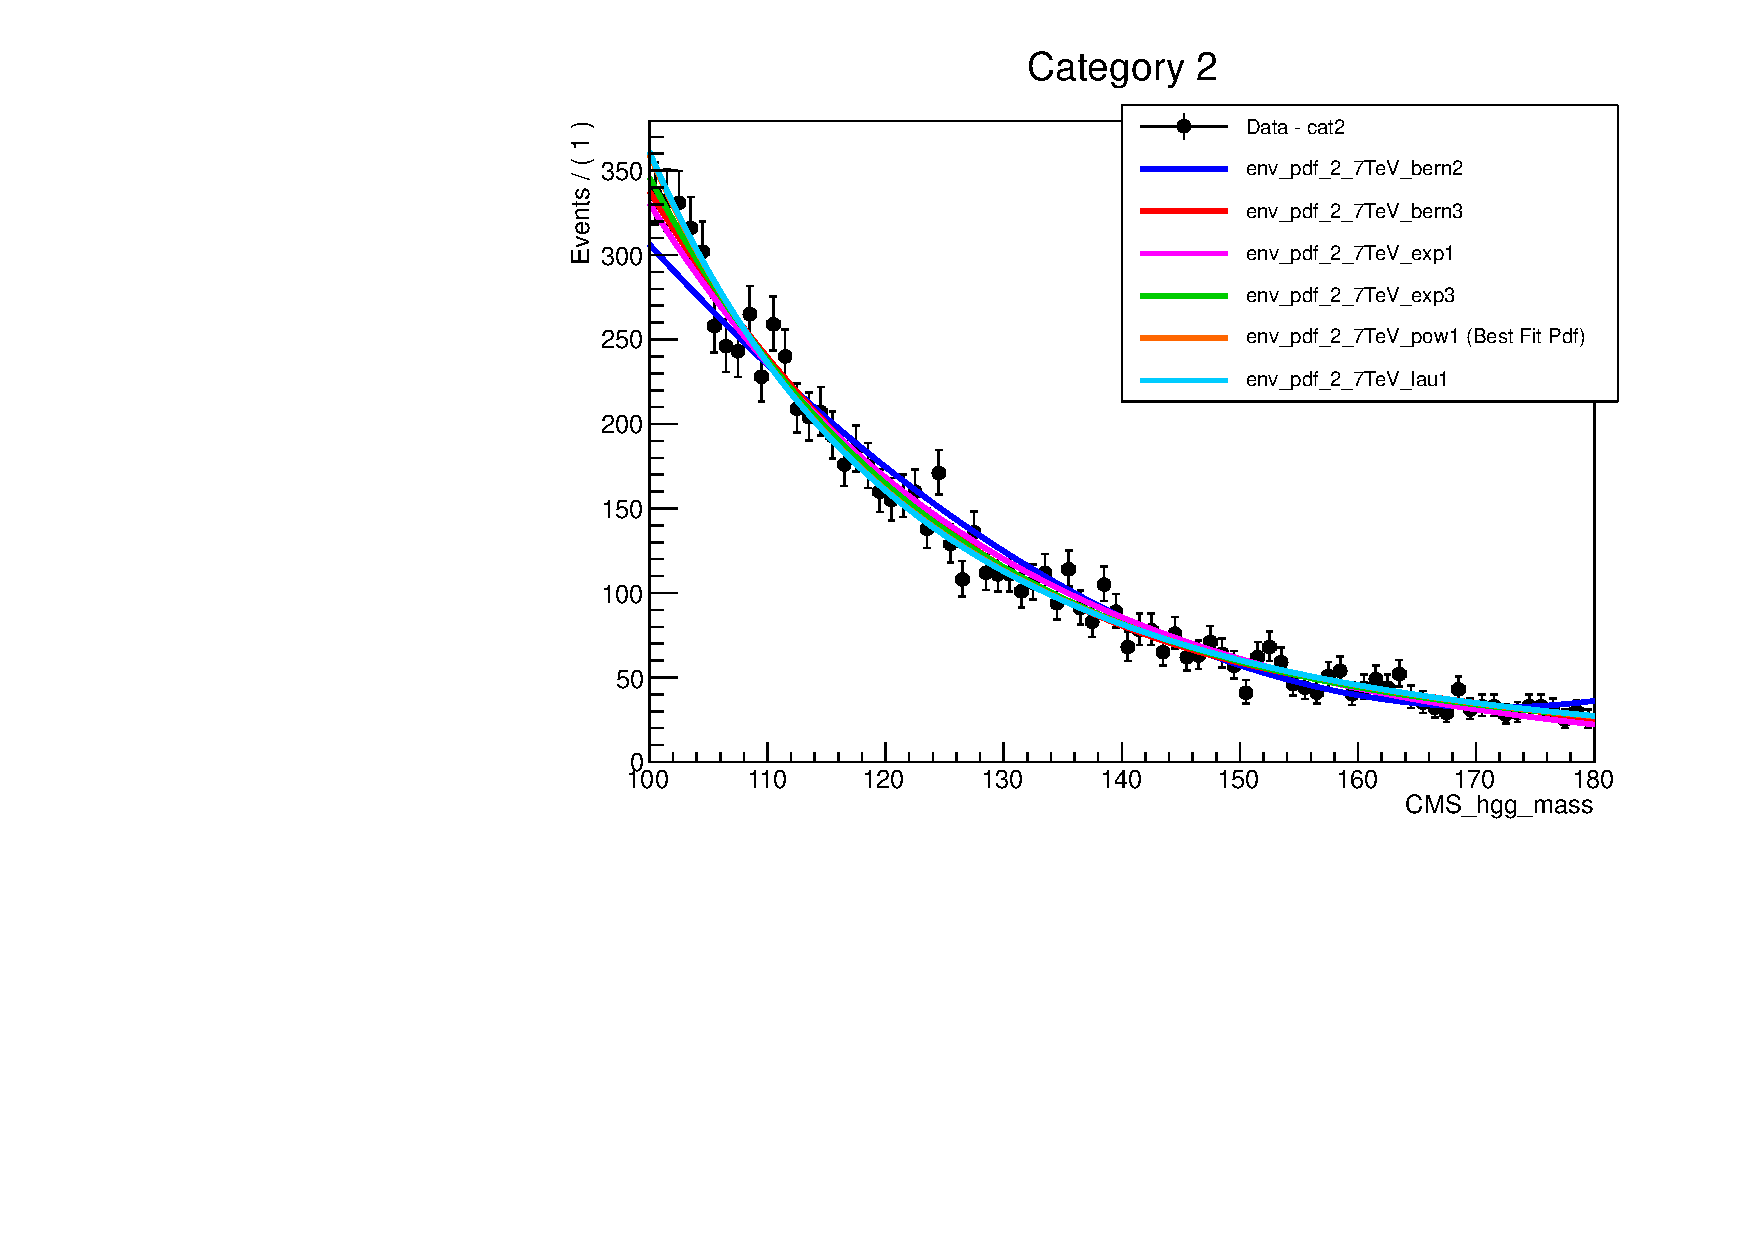
\includegraphics[width=0.49\textwidth]{ch5_anal_and_results/plots/mva_7TeV/multipdf_cat2.pdf}
  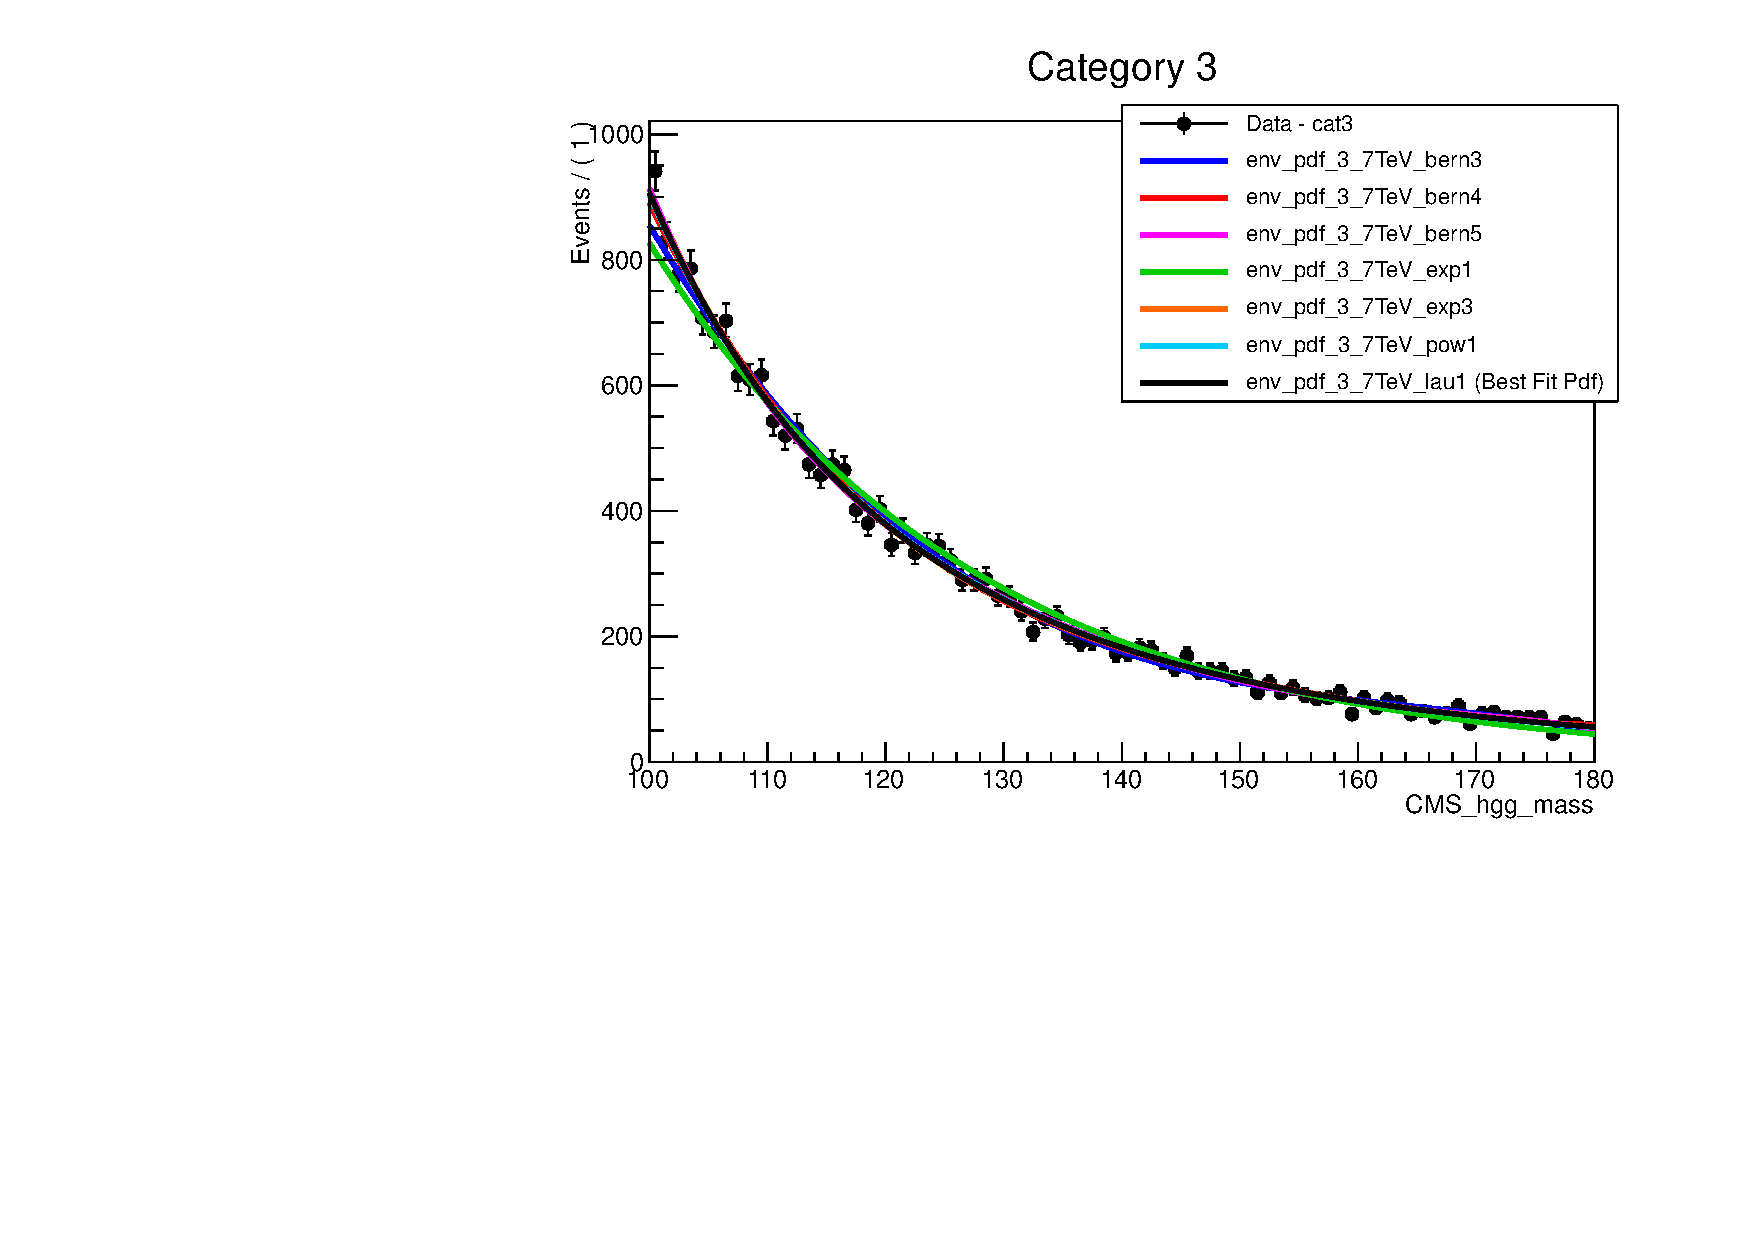
\includegraphics[width=0.49\textwidth]{ch5_anal_and_results/plots/mva_7TeV/multipdf_cat3.pdf}\\
  \caption{The diphoton invariant mass distribution and the function choices for the background envelope for the inclusive categories in the 7~\TeV dataset. \red{Category labels not numbers?}}
  \label{fig:multipdf1}
\end{figure}

\begin{figure}
  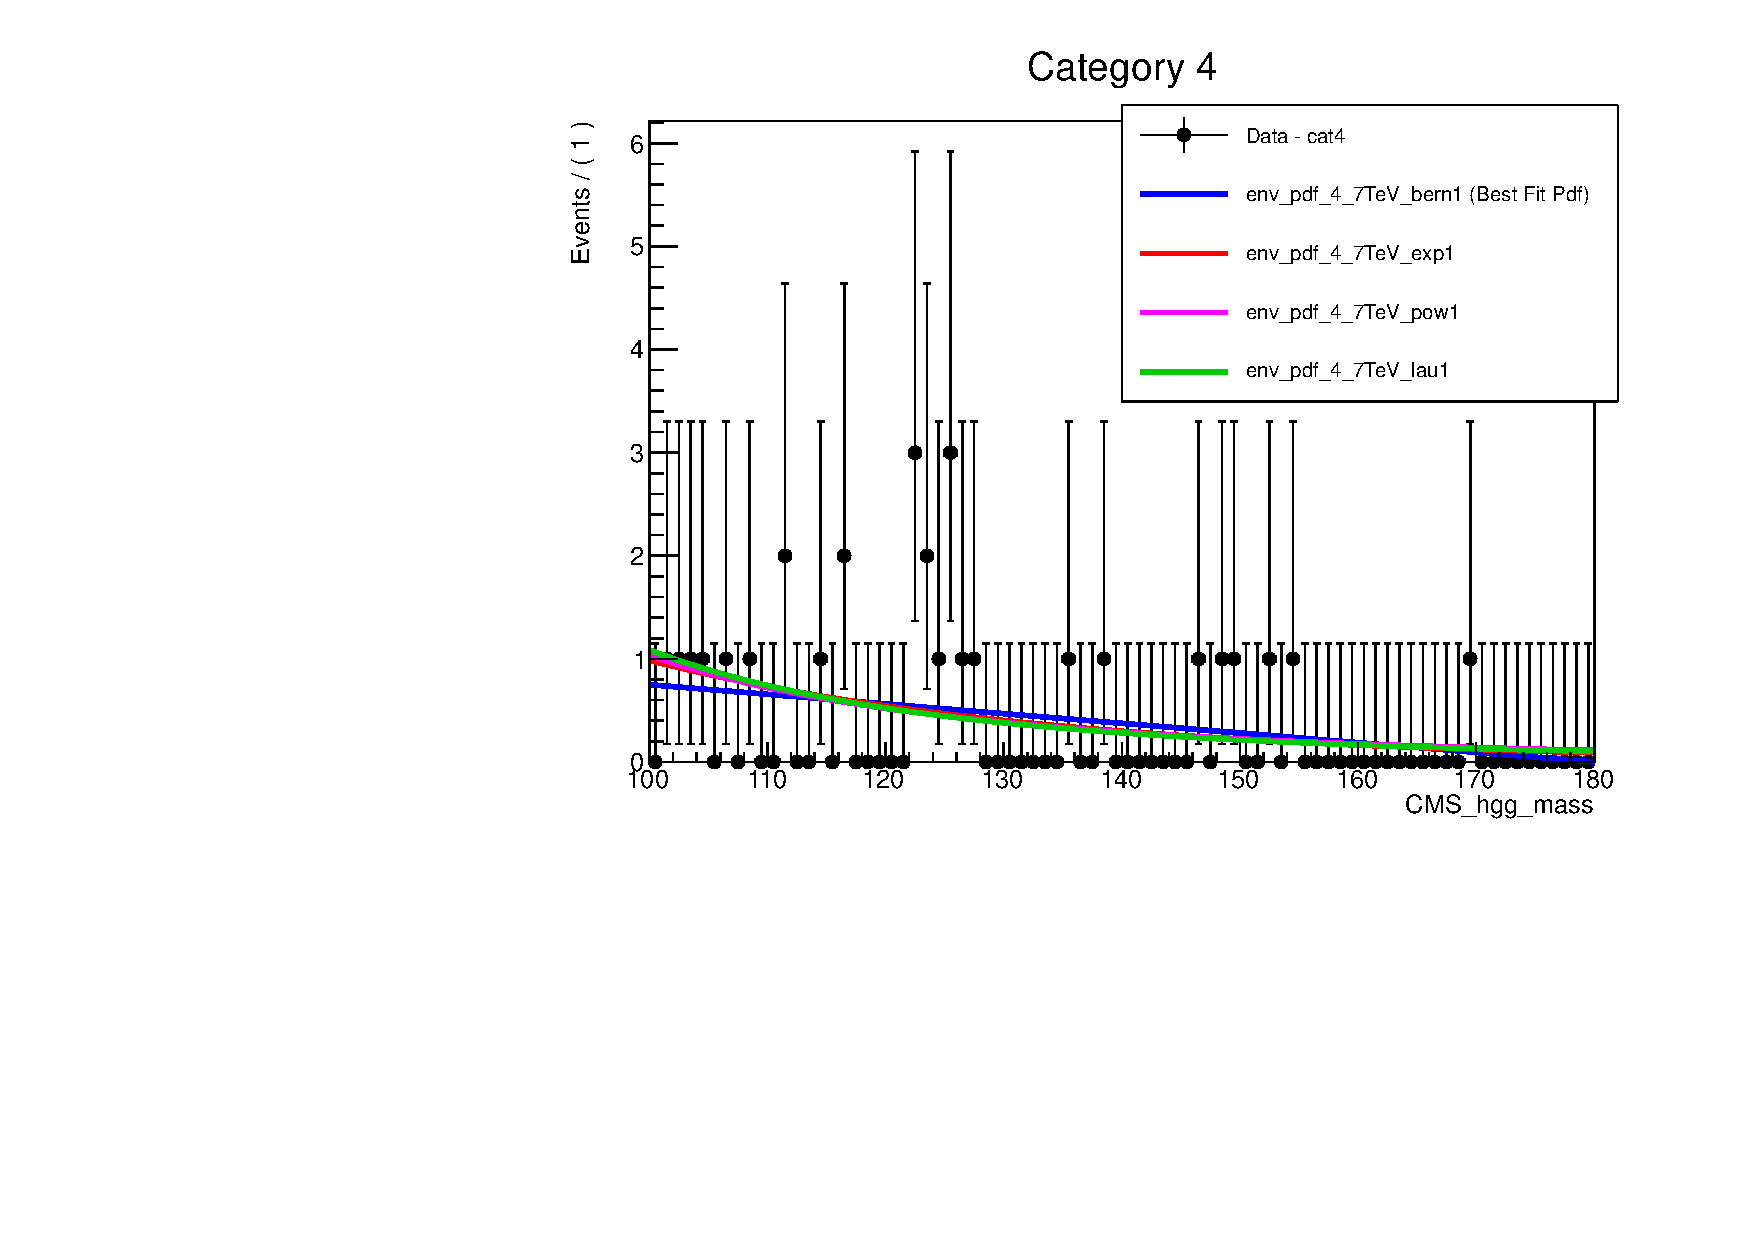
\includegraphics[width=0.49\textwidth]{ch5_anal_and_results/plots/mva_7TeV/multipdf_cat4.pdf}
  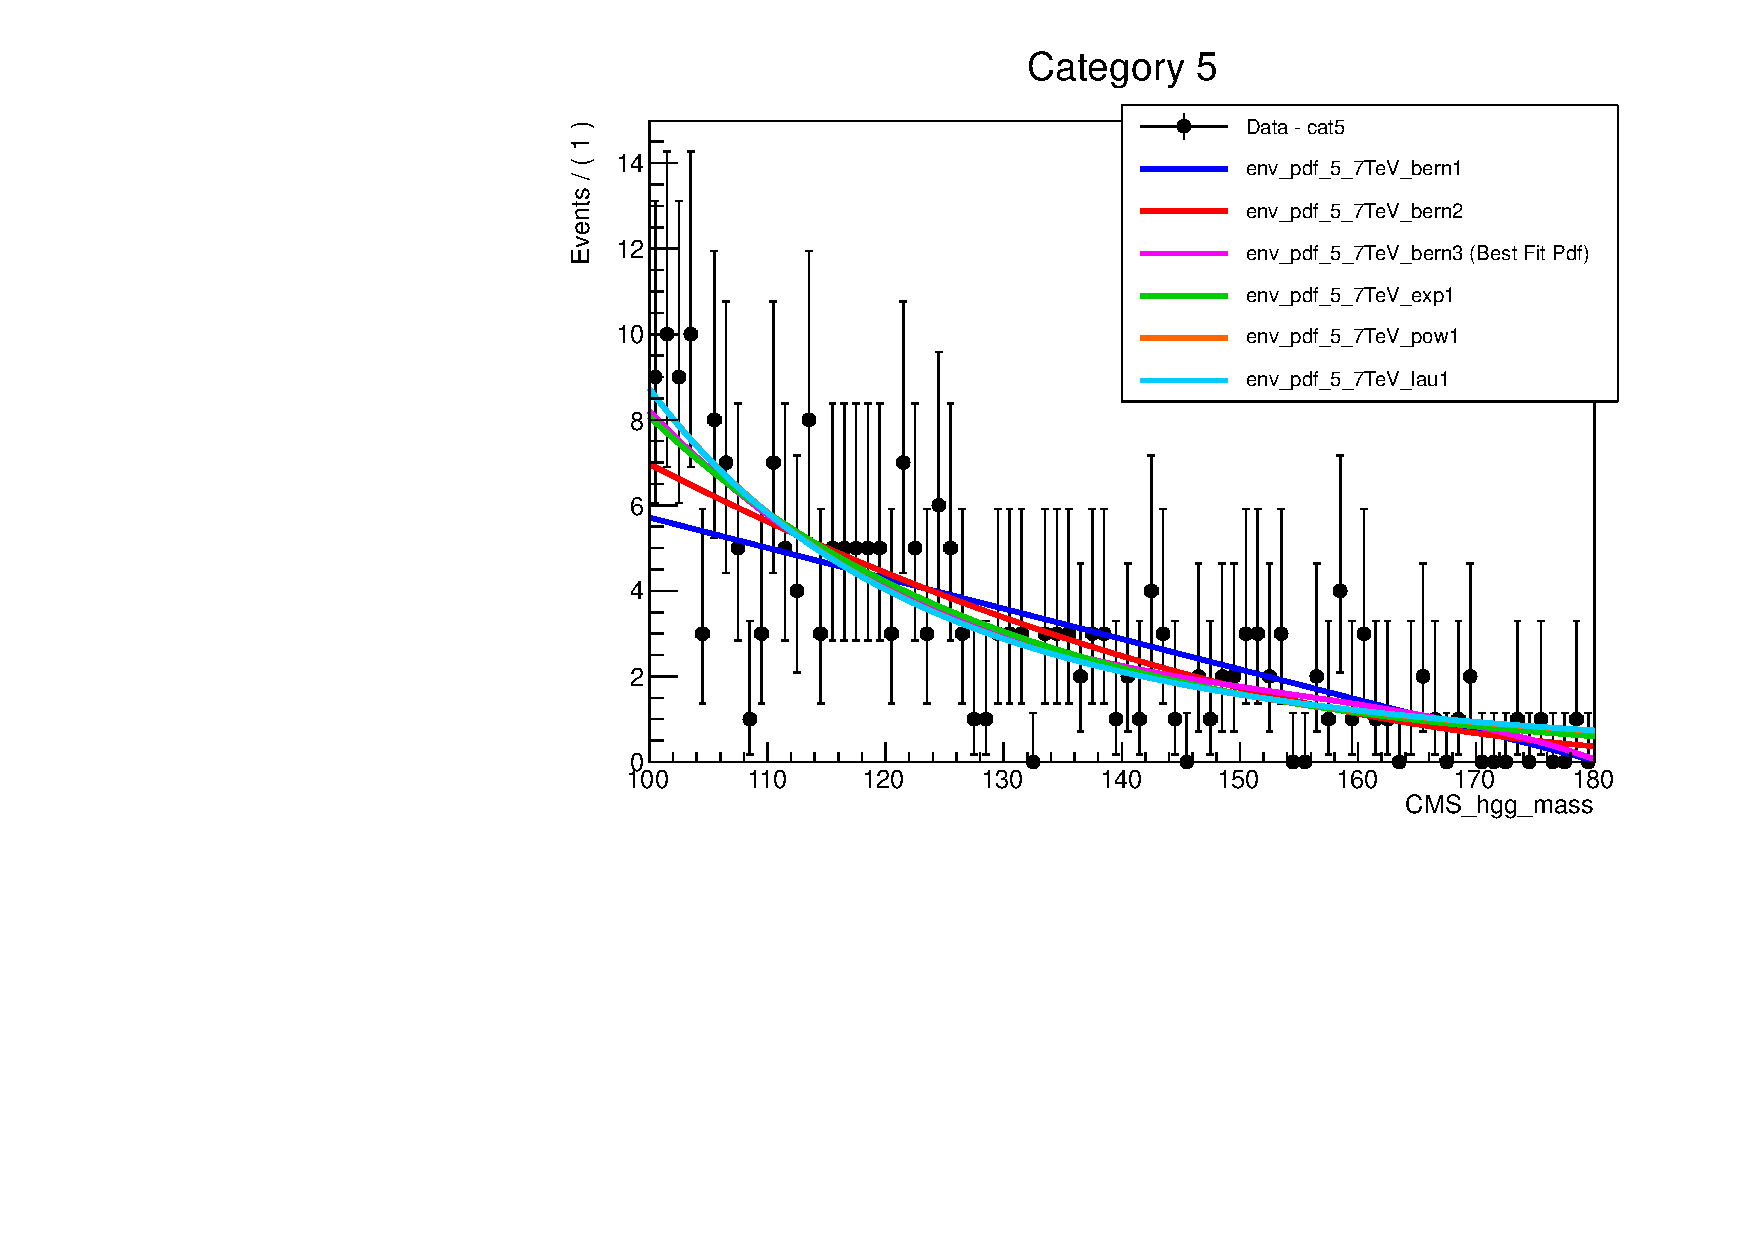
\includegraphics[width=0.49\textwidth]{ch5_anal_and_results/plots/mva_7TeV/multipdf_cat5.pdf}\\
  \caption{The diphoton invariant mass distribution and the function choices for the background envelope for the dijet categories in the 7~\TeV dataset. \red{Category labels not numbers?}}
  \label{fig:multipdf2}
\end{figure}

\begin{figure}
  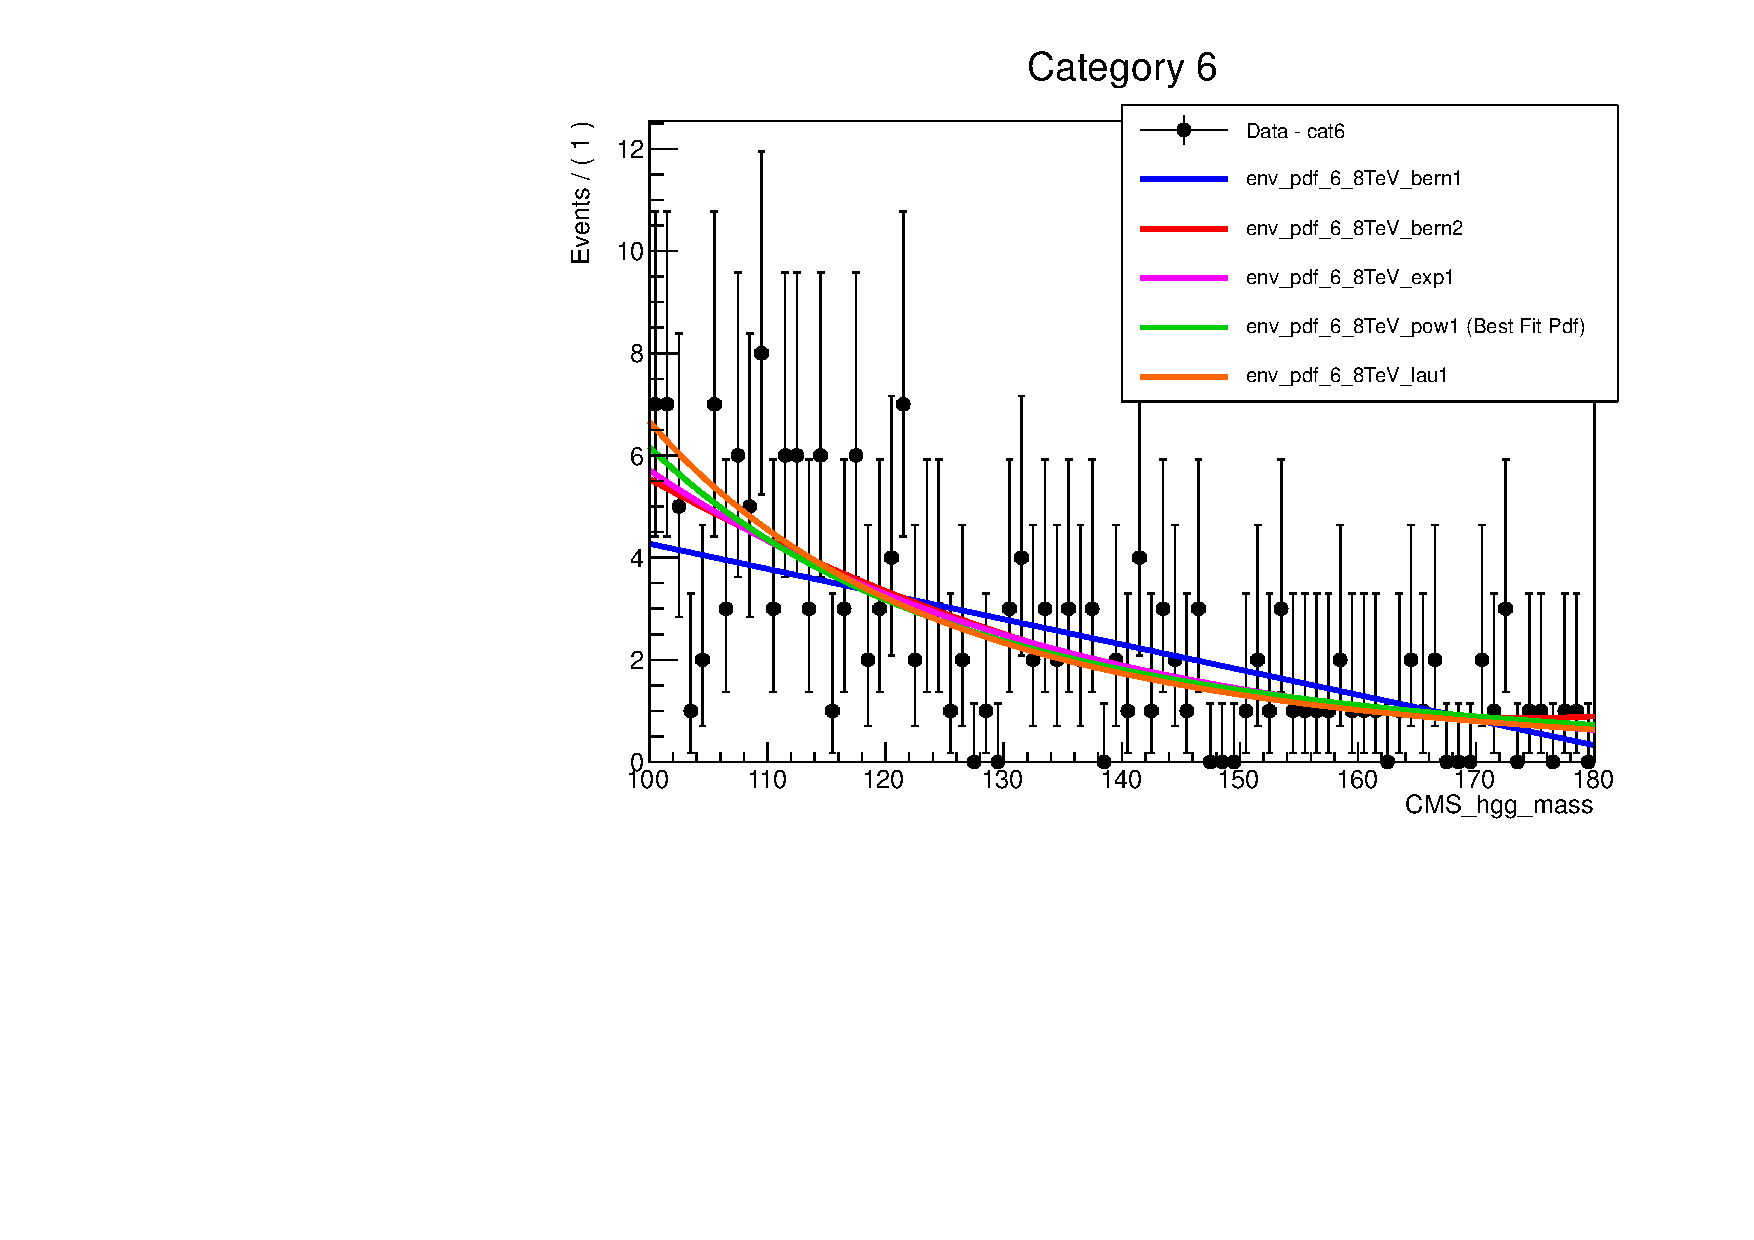
\includegraphics[width=0.49\textwidth]{ch5_anal_and_results/plots/mva_8TeV/multipdf_cat6.pdf}
  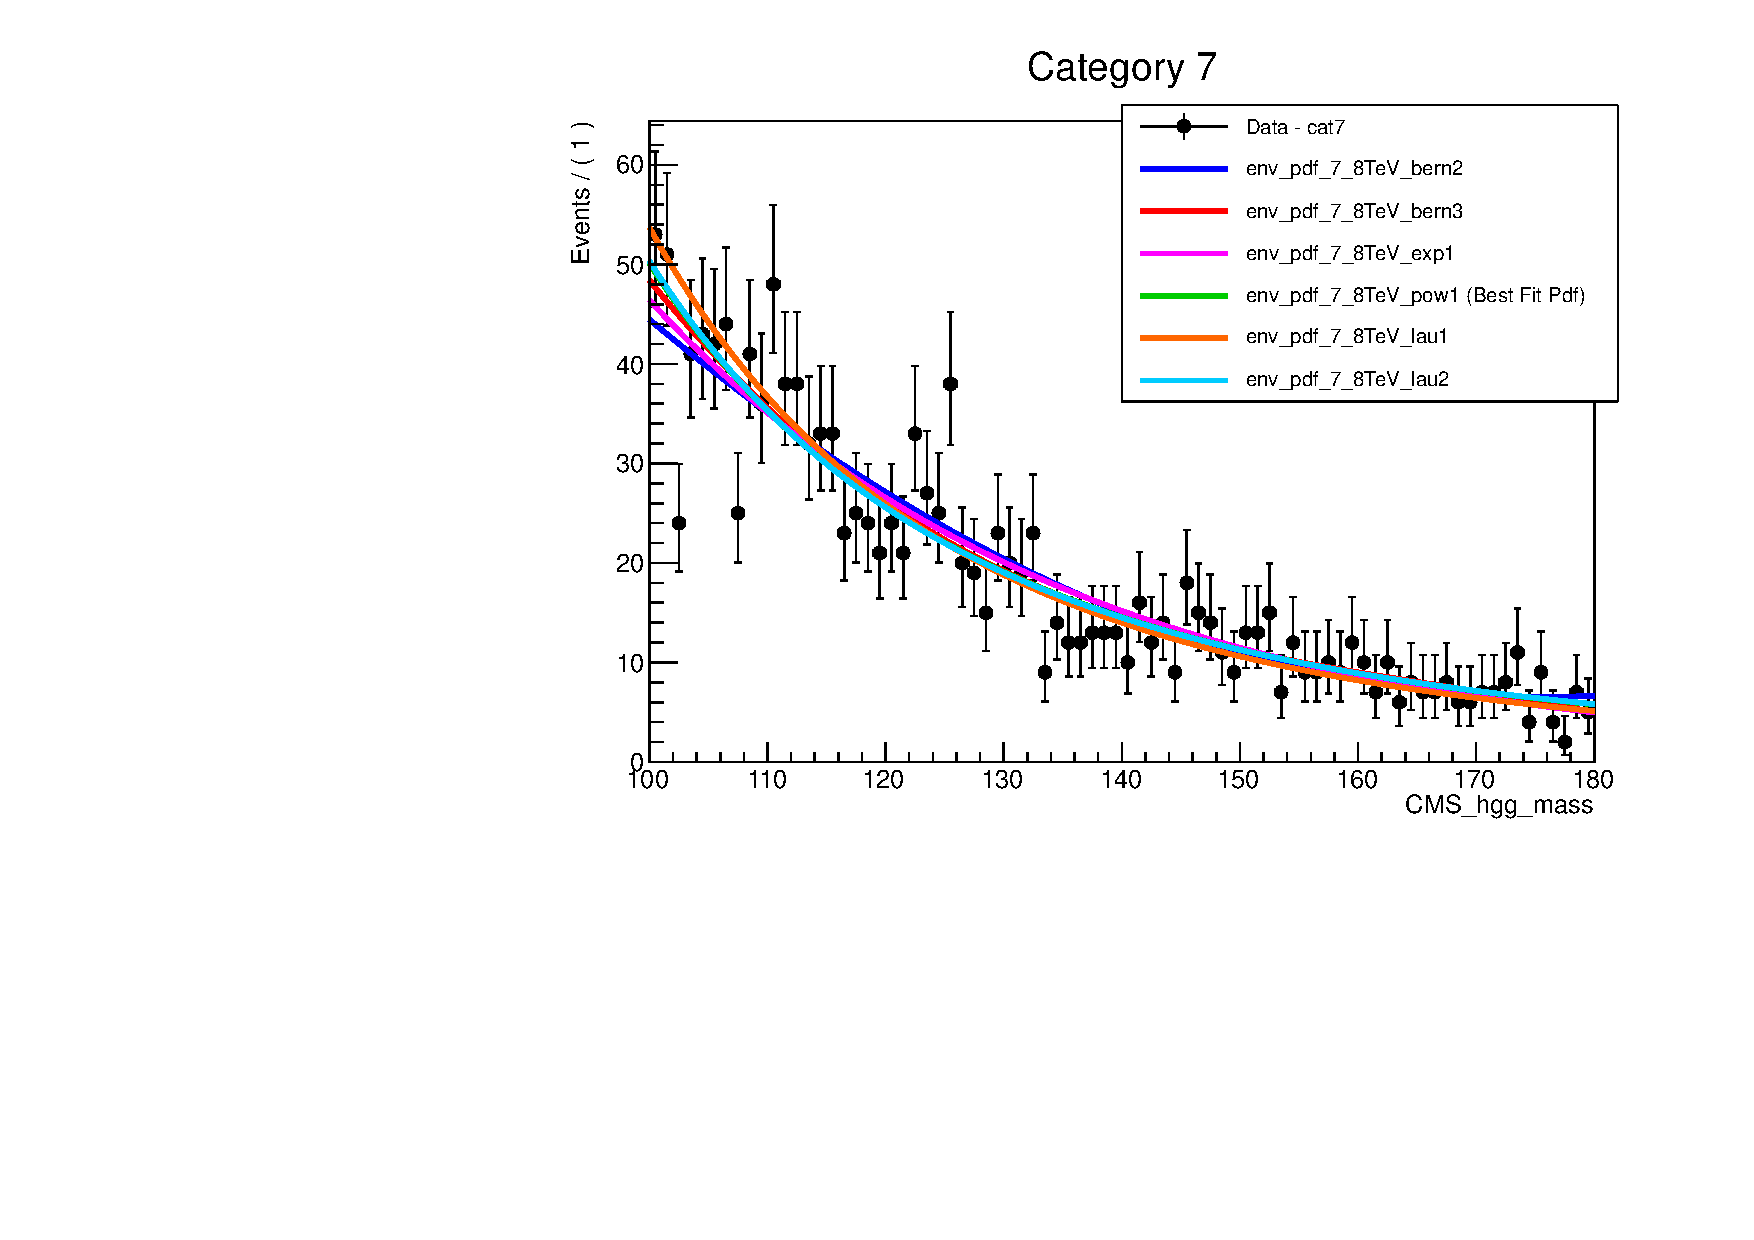
\includegraphics[width=0.49\textwidth]{ch5_anal_and_results/plots/mva_8TeV/multipdf_cat7.pdf}\\
  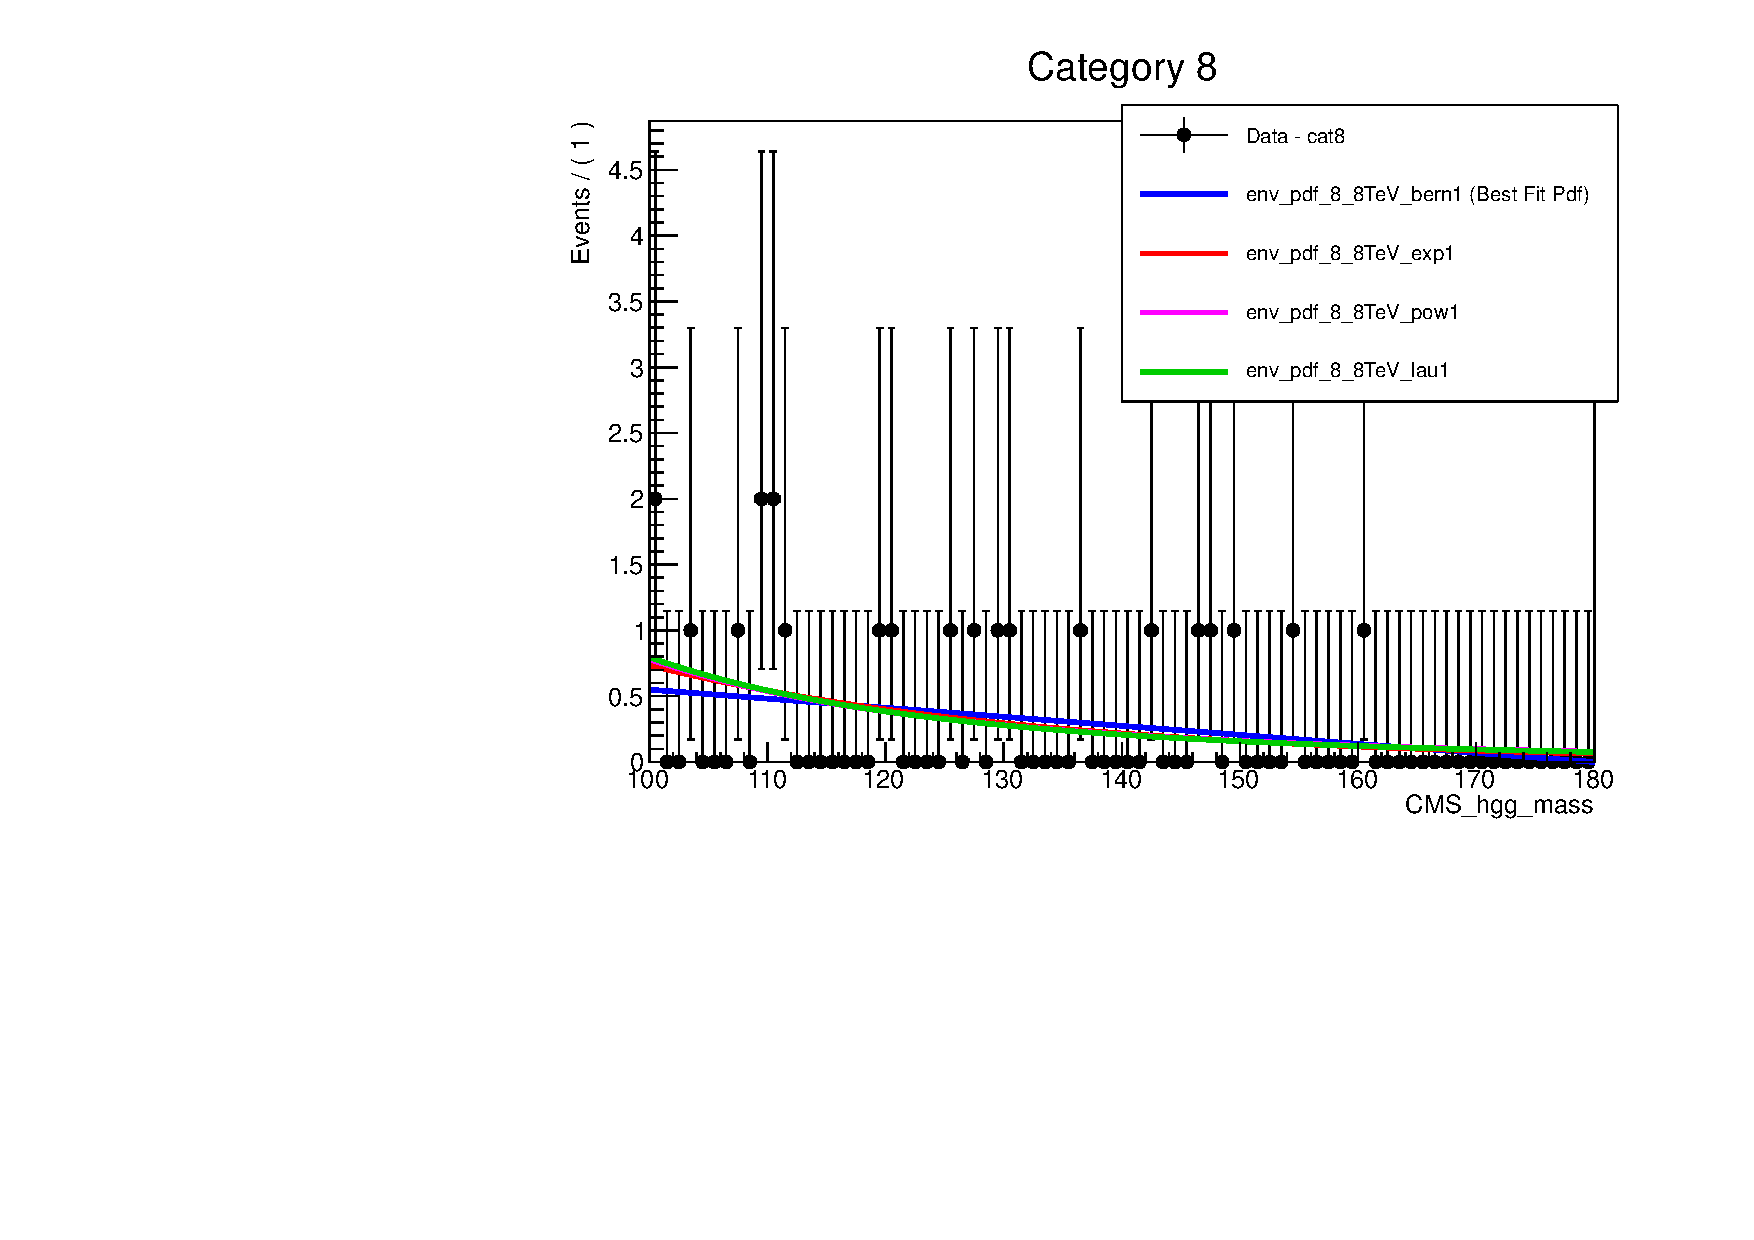
\includegraphics[width=0.49\textwidth]{ch5_anal_and_results/plots/mva_8TeV/multipdf_cat8.pdf}
  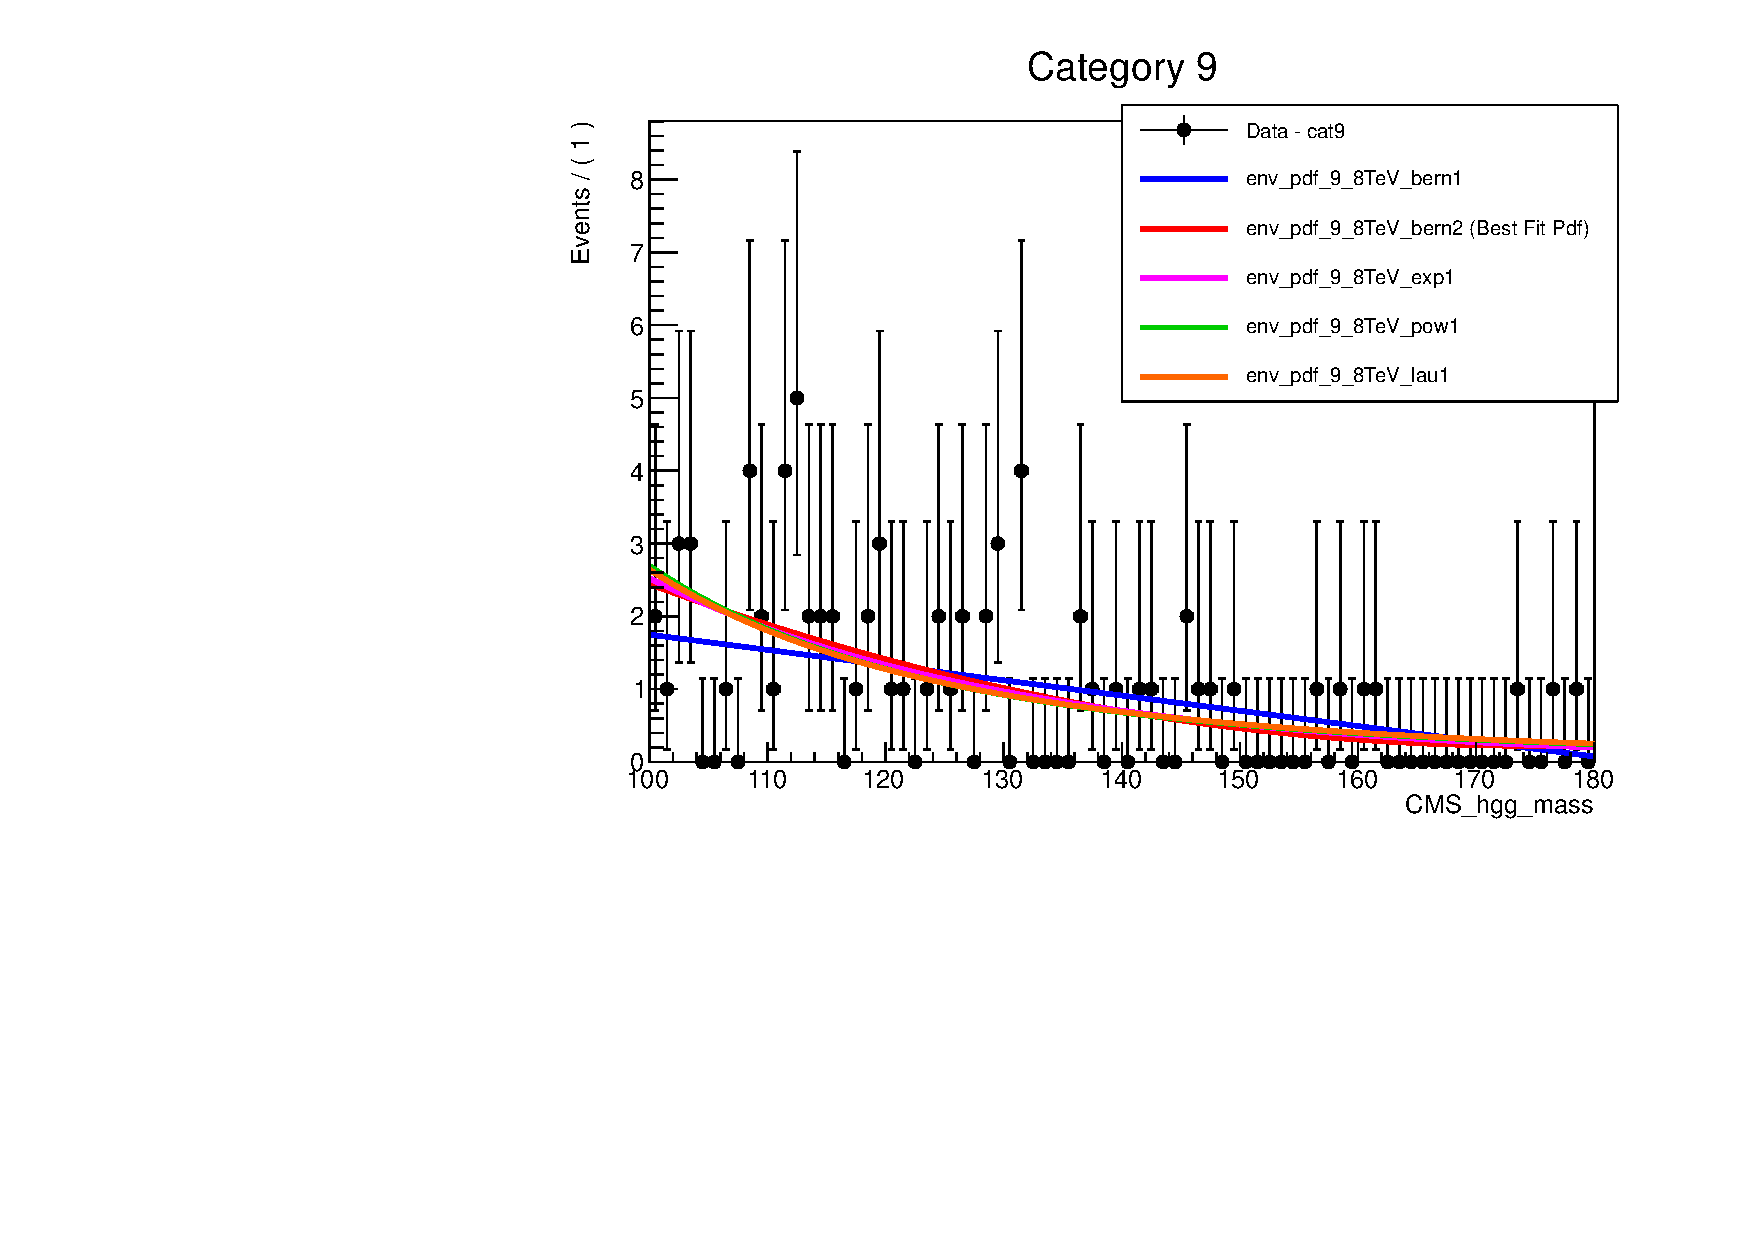
\includegraphics[width=0.49\textwidth]{ch5_anal_and_results/plots/mva_8TeV/multipdf_cat9.pdf}\\
  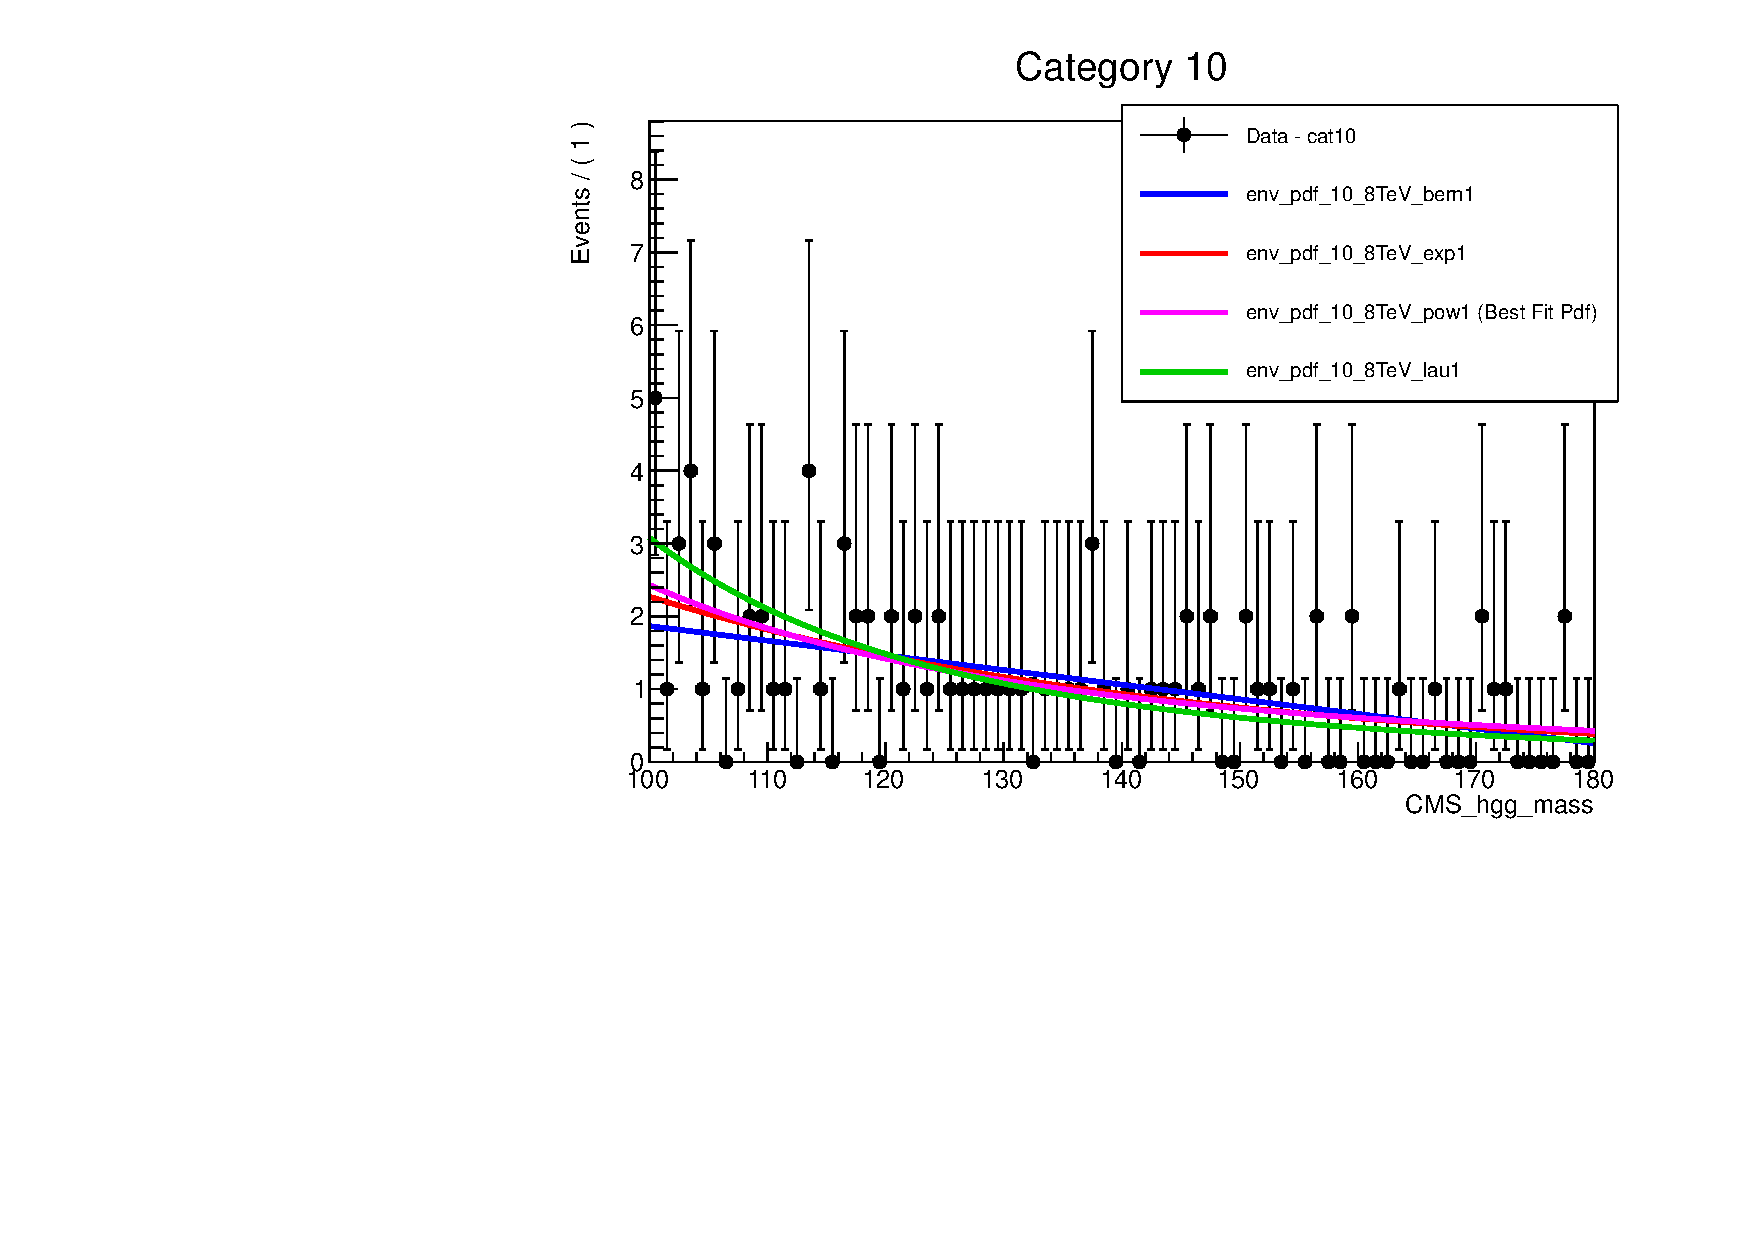
\includegraphics[width=0.49\textwidth]{ch5_anal_and_results/plots/mva_8TeV/multipdf_cat10.pdf}
  \caption{The diphoton invariant mass distribution and the function choices for the background envelope for the \VH and \ttH categories in the 7~\TeV dataset. \red{Category labels not numbers?}}
  \label{fig:multipdf3}
\end{figure}

\begin{figure}
  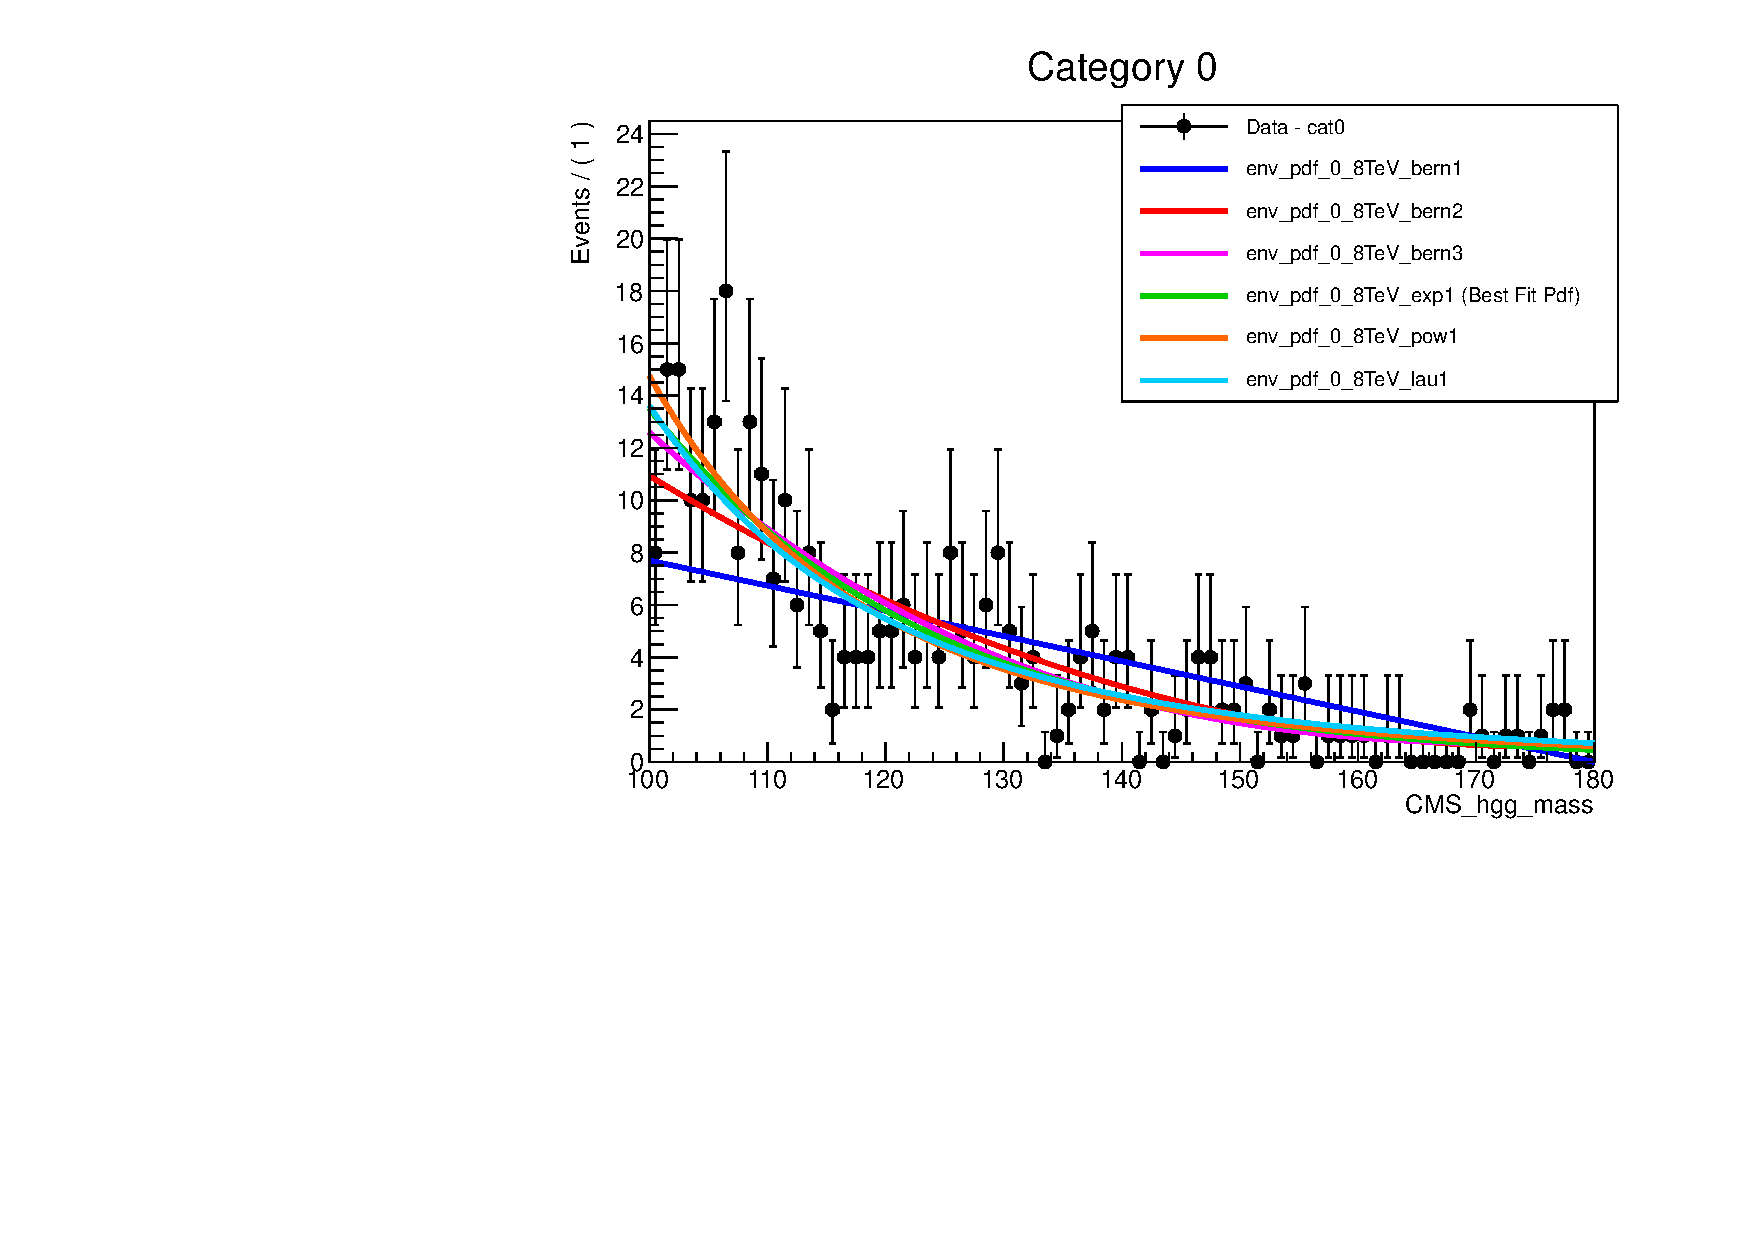
\includegraphics[width=0.49\textwidth]{ch5_anal_and_results/plots/mva_8TeV/multipdf_cat0.pdf}
  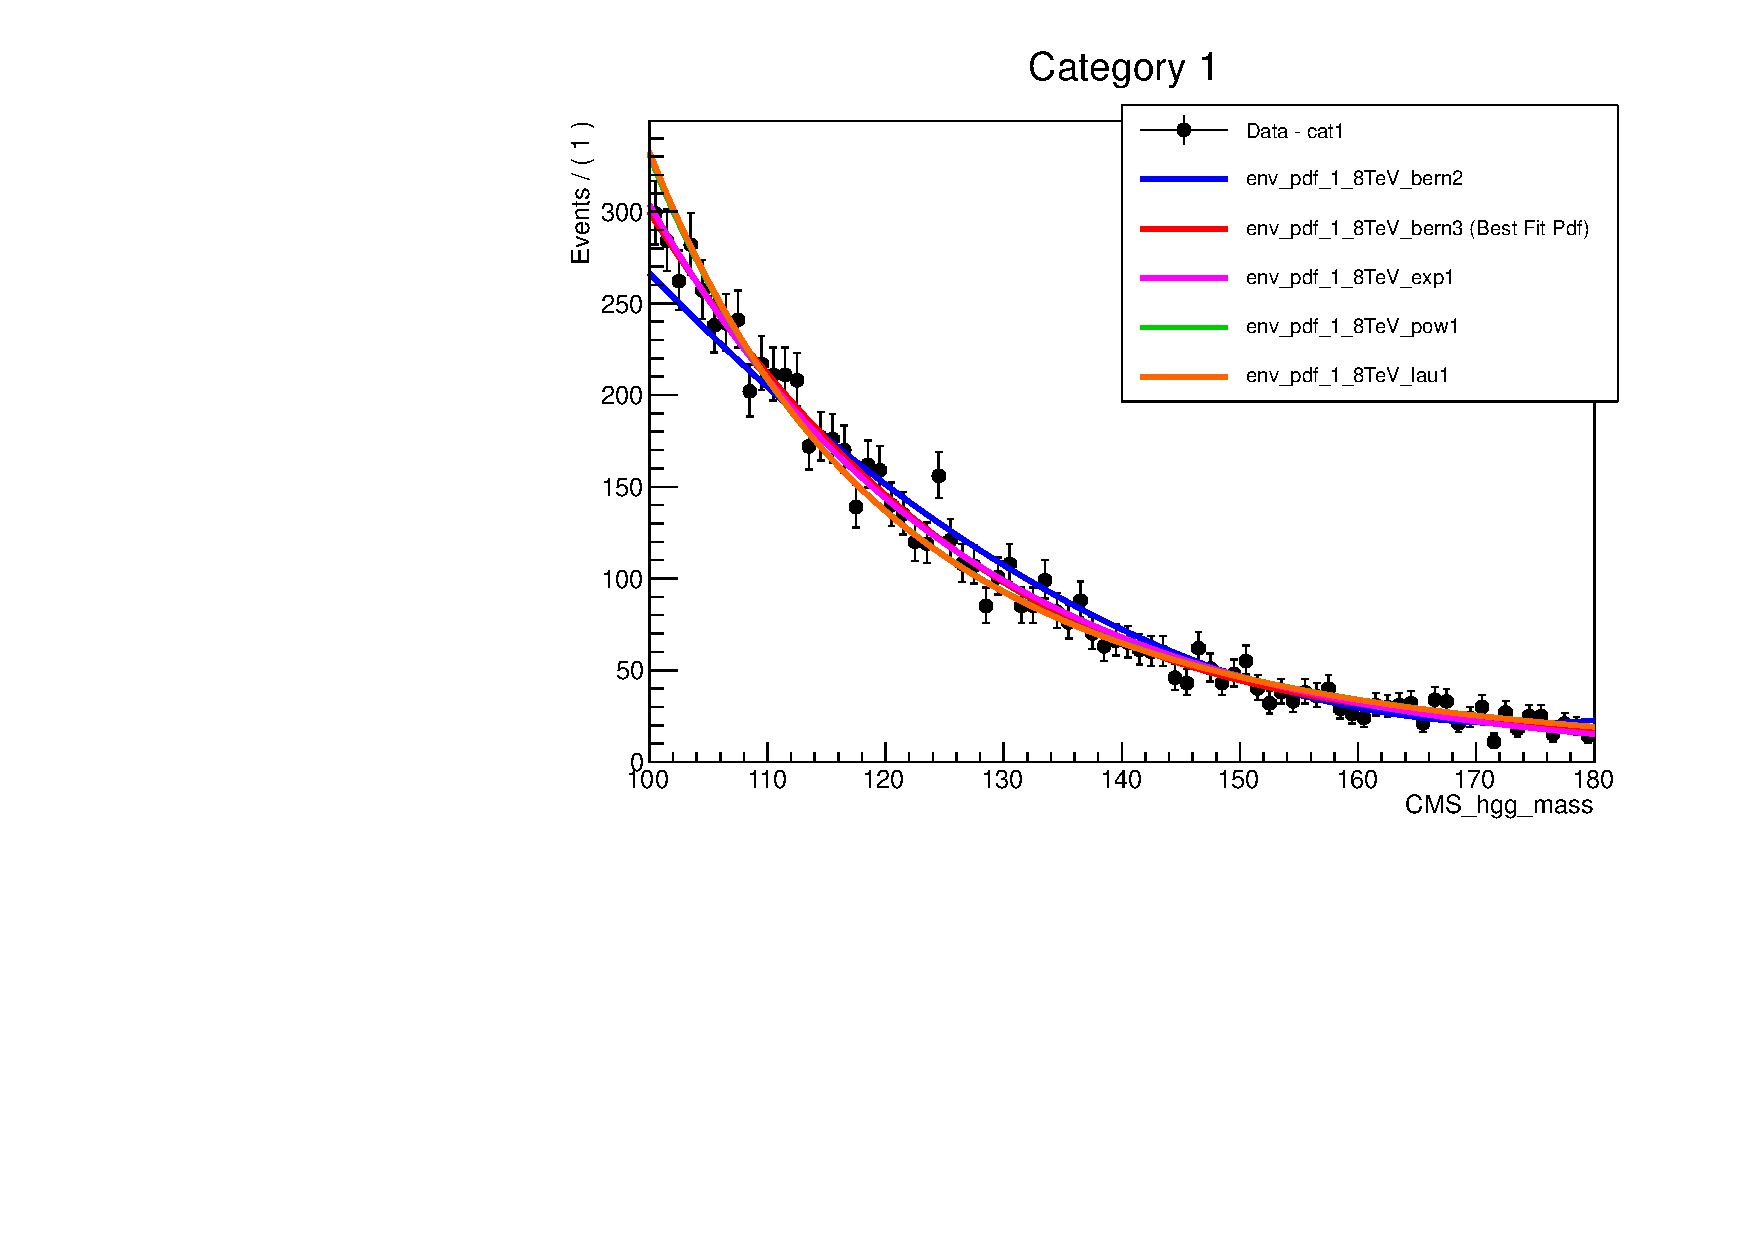
\includegraphics[width=0.49\textwidth]{ch5_anal_and_results/plots/mva_8TeV/multipdf_cat1.pdf}\\
  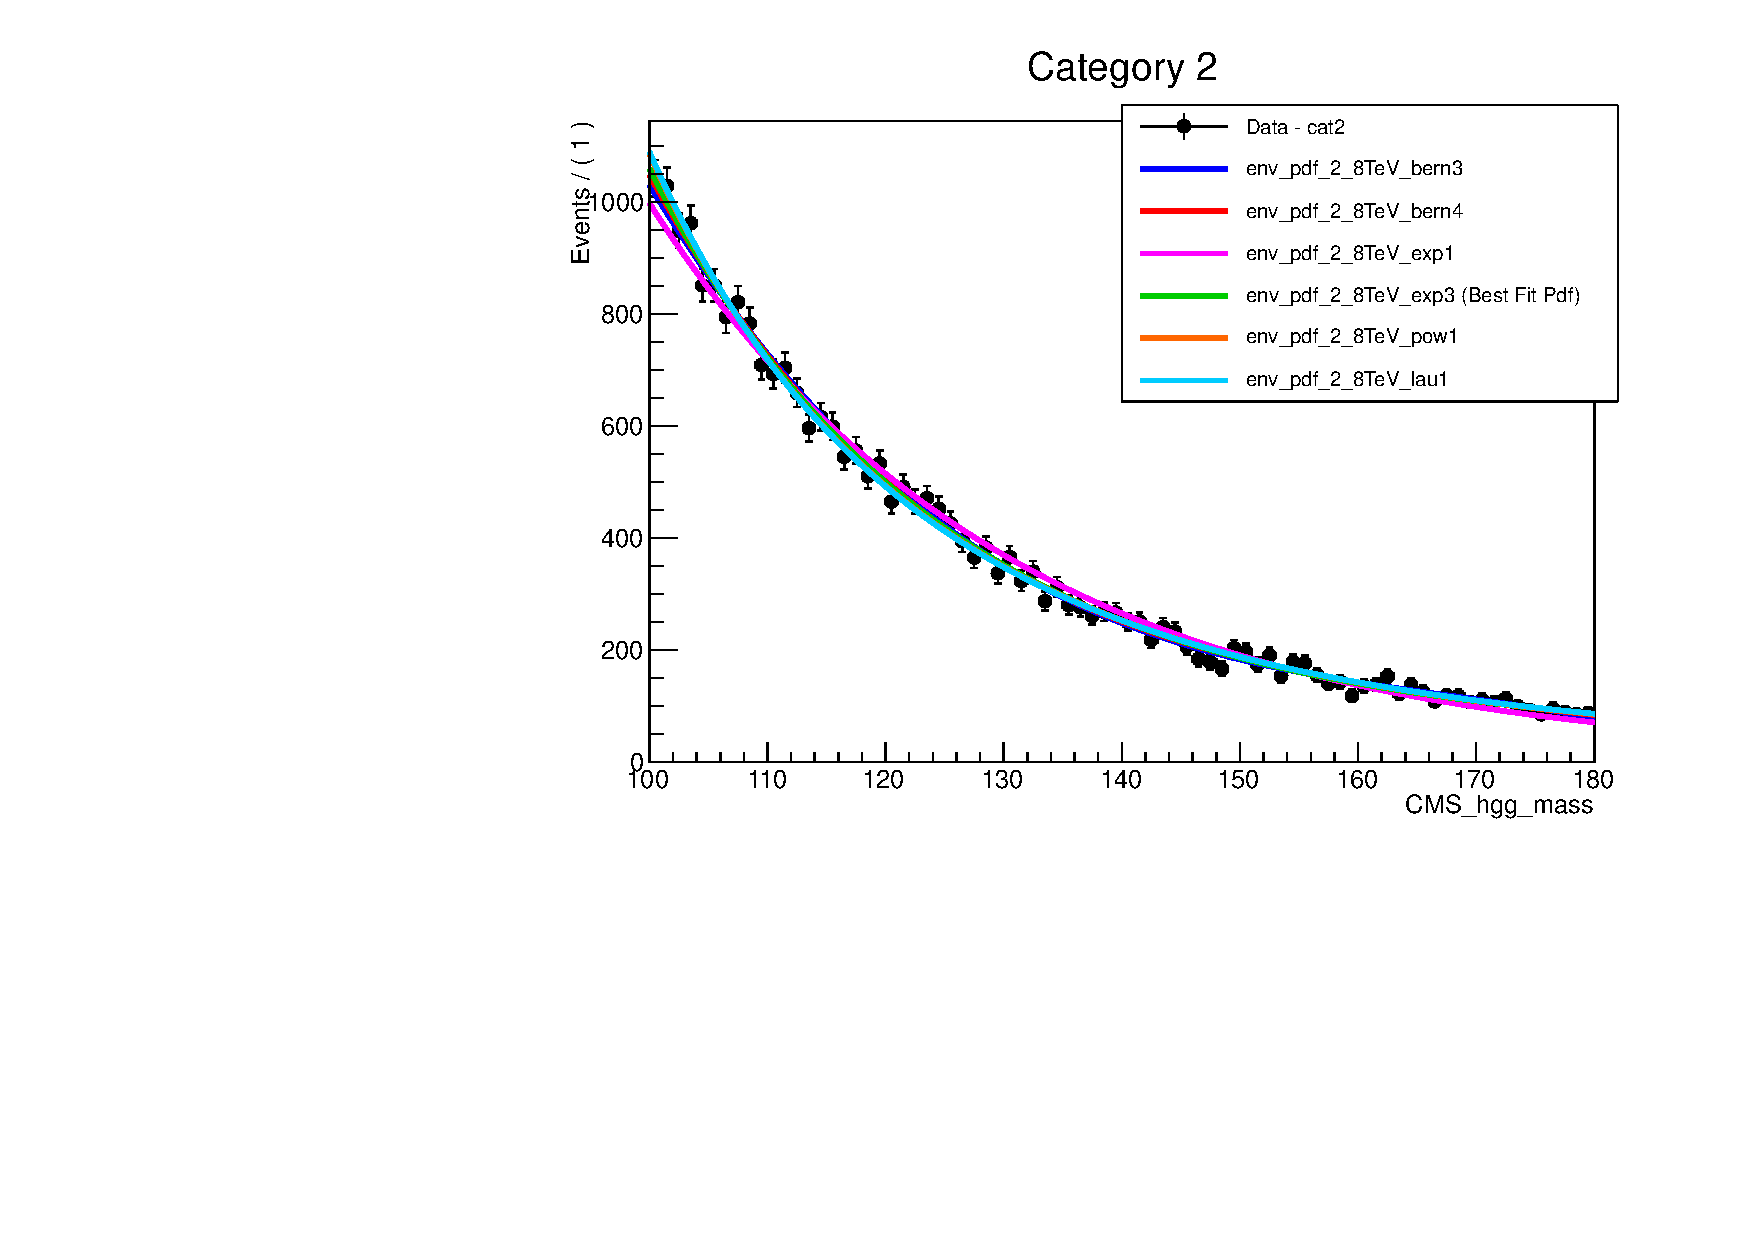
\includegraphics[width=0.49\textwidth]{ch5_anal_and_results/plots/mva_8TeV/multipdf_cat2.pdf}
  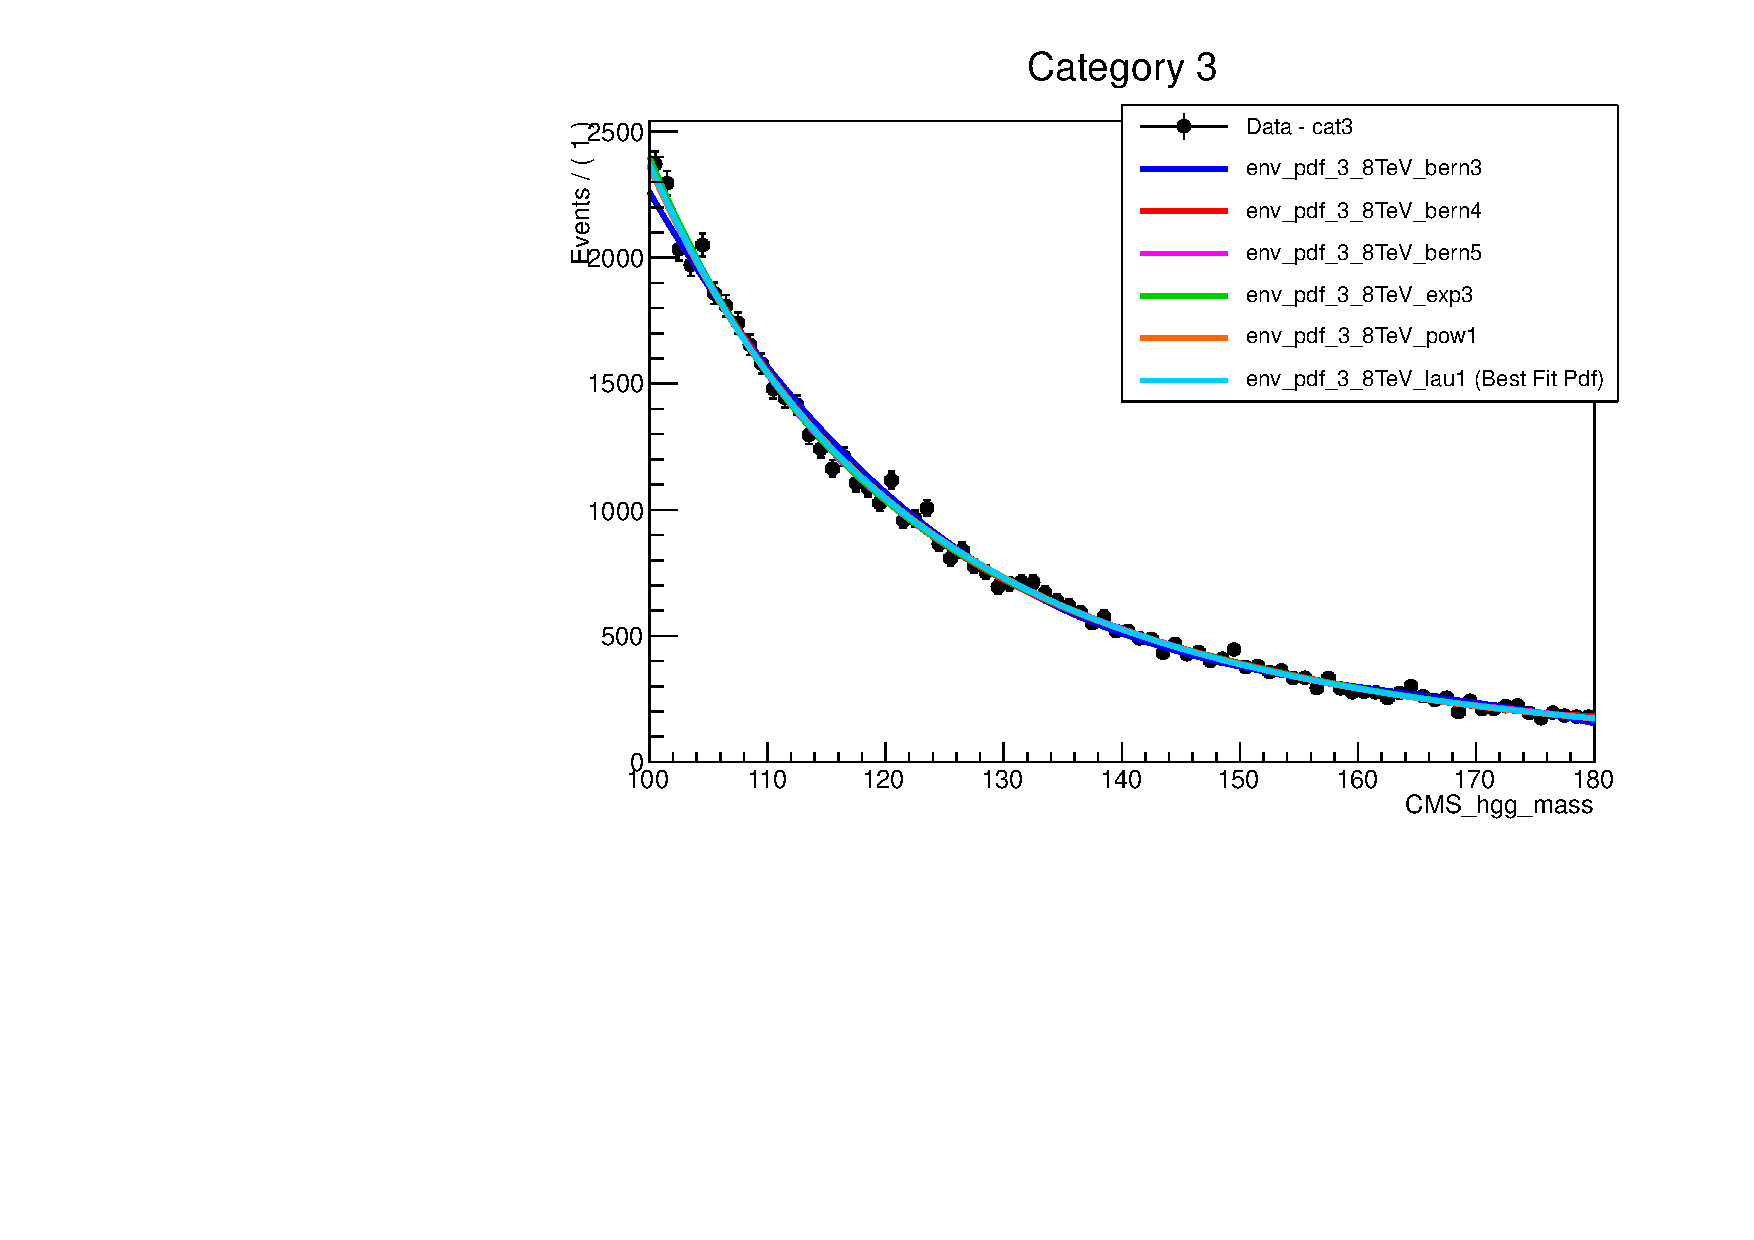
\includegraphics[width=0.49\textwidth]{ch5_anal_and_results/plots/mva_8TeV/multipdf_cat3.pdf}\\
  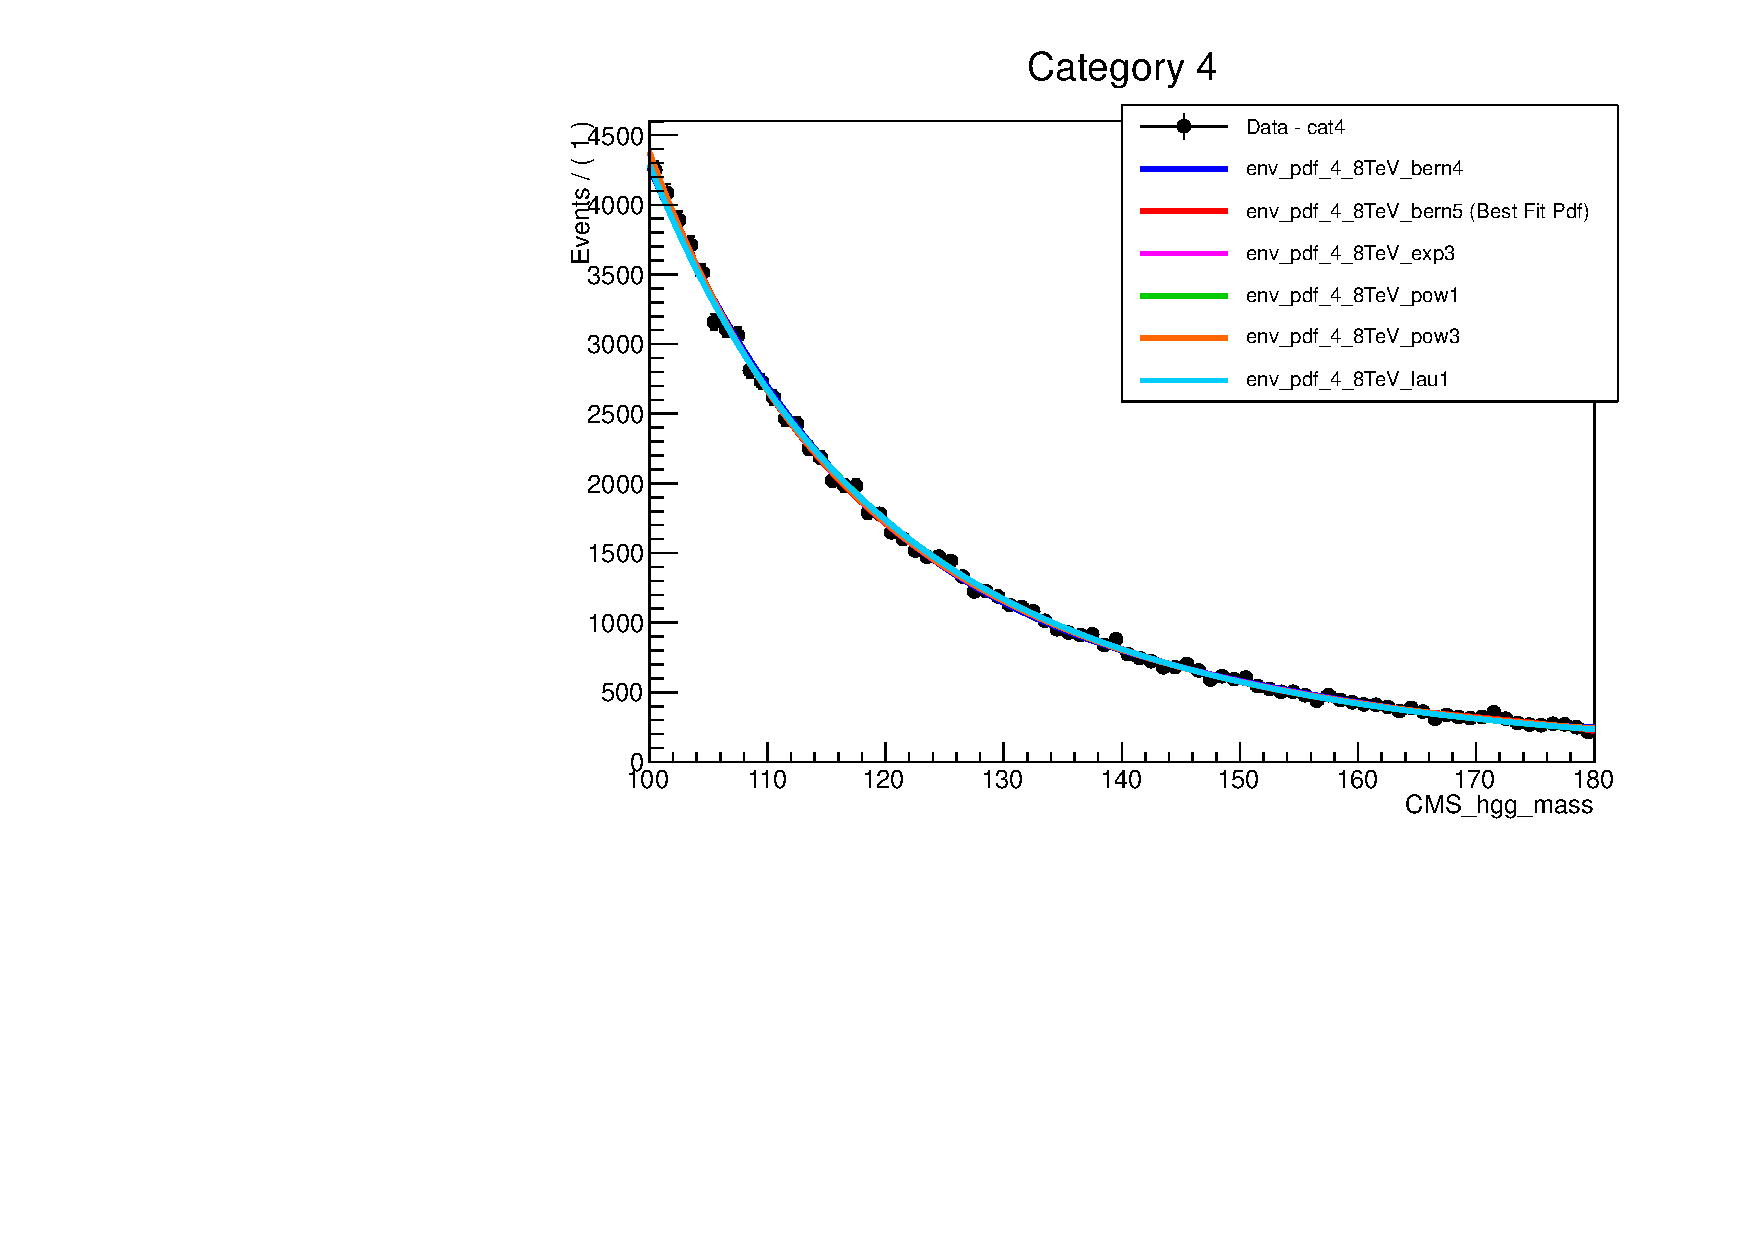
\includegraphics[width=0.49\textwidth]{ch5_anal_and_results/plots/mva_8TeV/multipdf_cat4.pdf}
  \caption{The diphoton invariant mass distribution and the function choices for the background envelope for the inclusive categories in the 8~\TeV dataset. \red{Category labels not numbers?}}
  \label{fig:multipdf4}
\end{figure}

\begin{figure}
  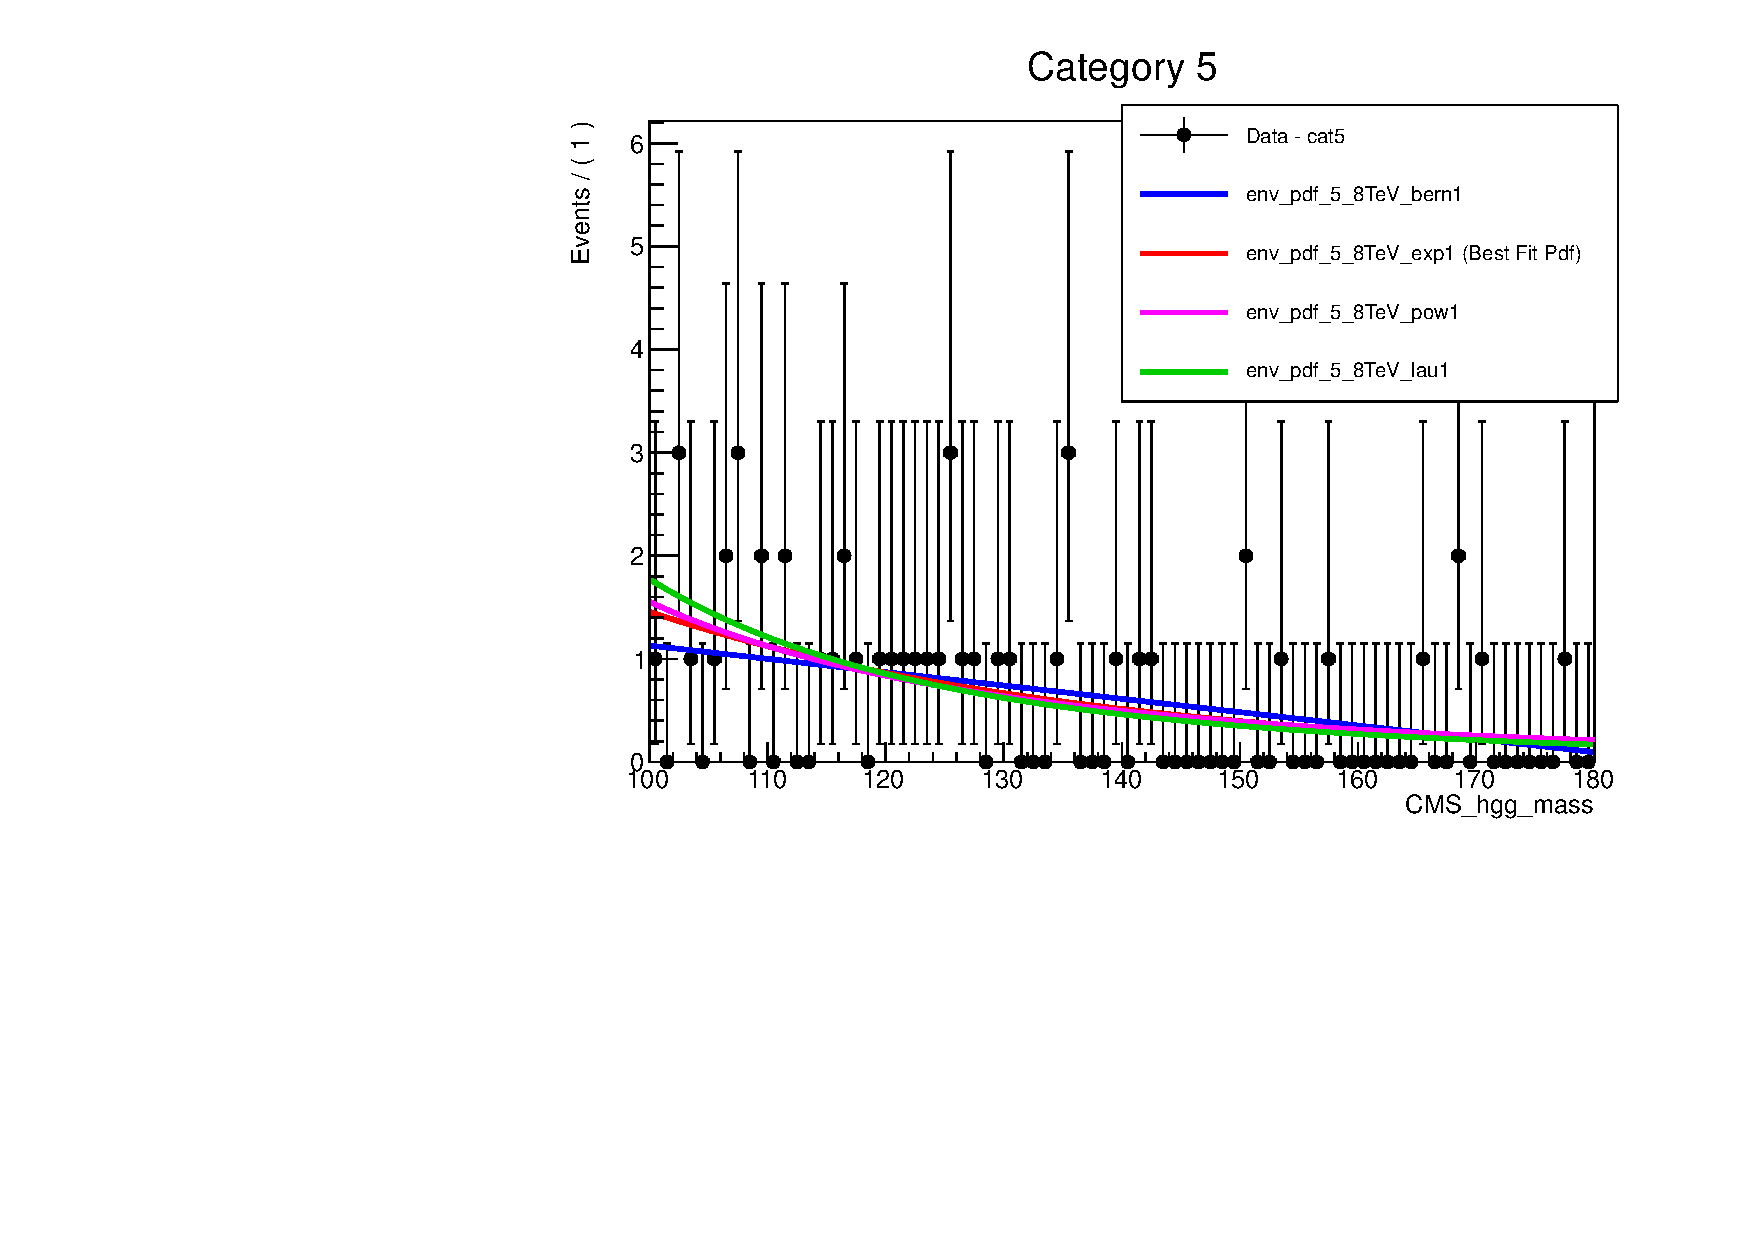
\includegraphics[width=0.49\textwidth]{ch5_anal_and_results/plots/mva_8TeV/multipdf_cat5.pdf}
  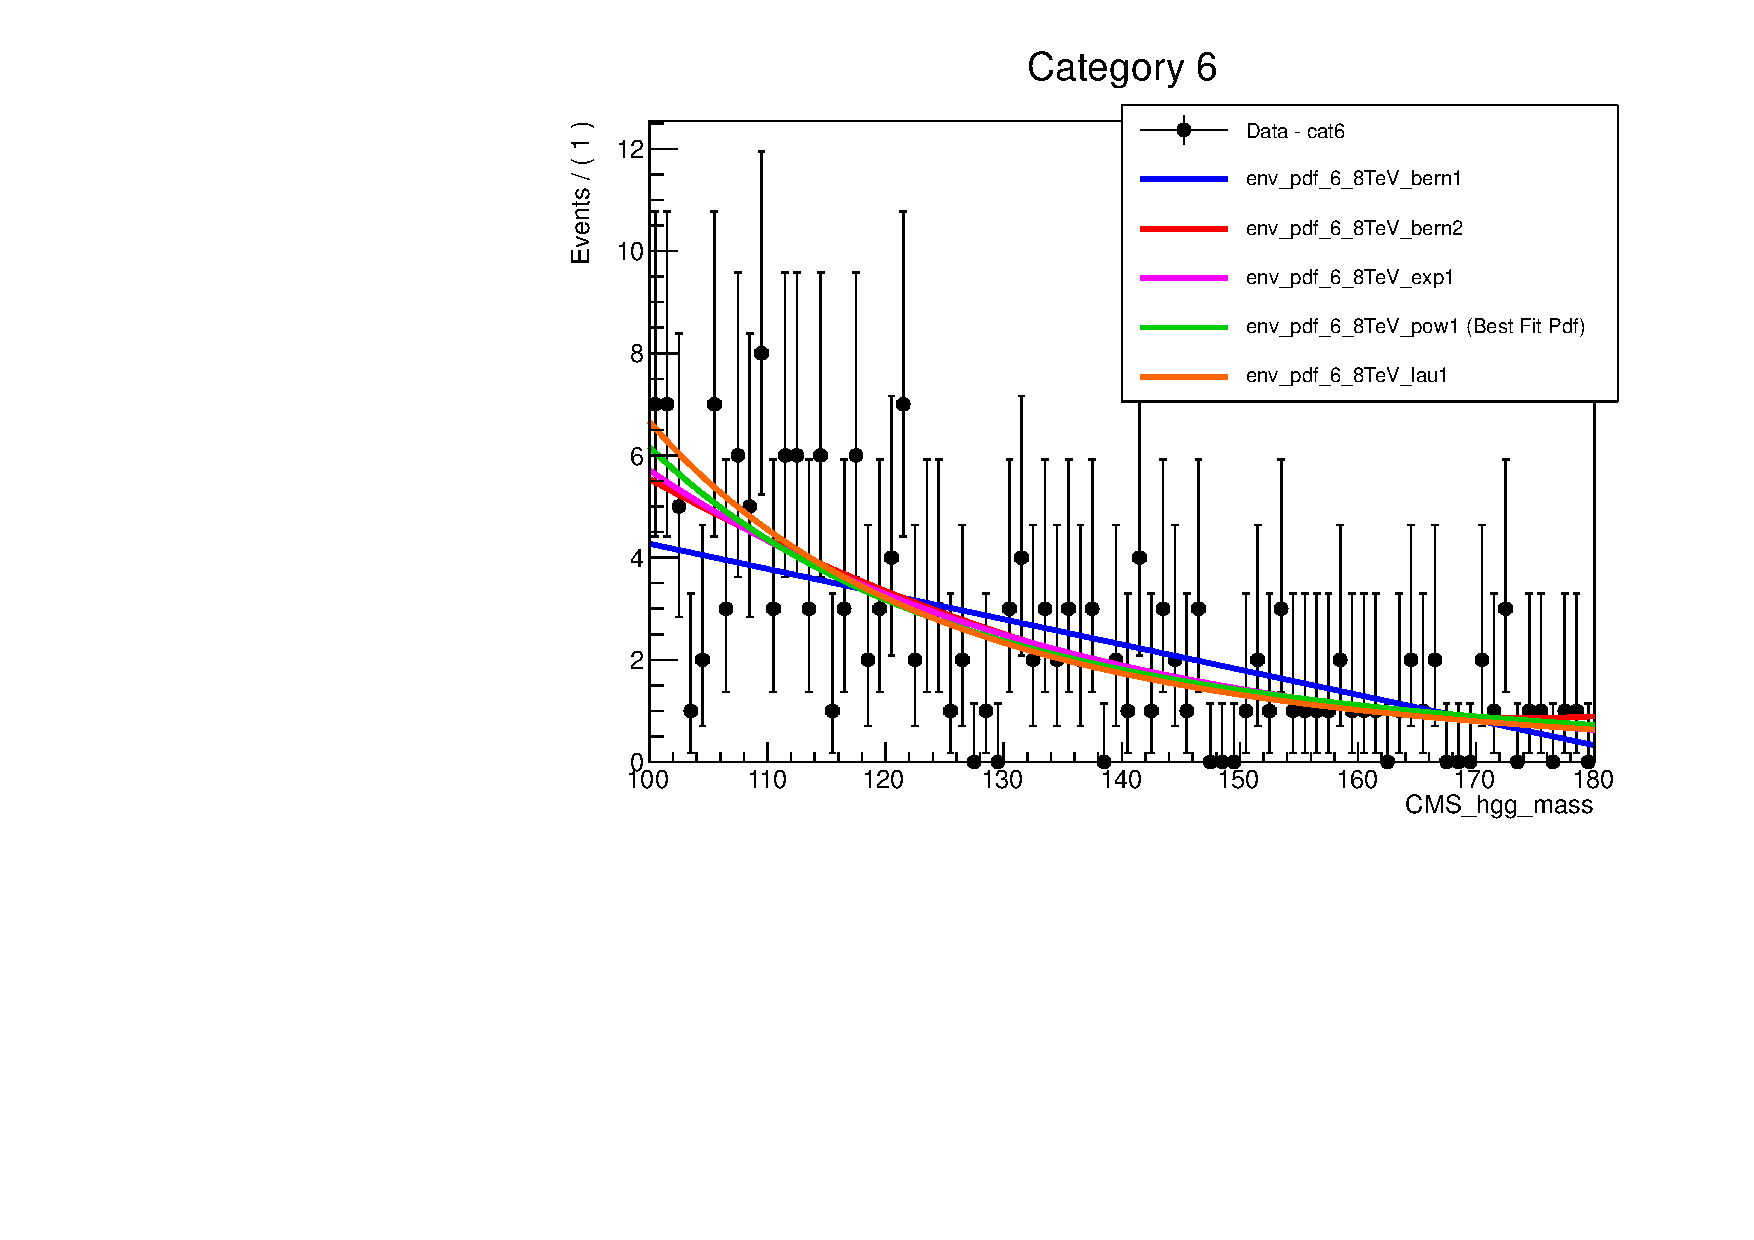
\includegraphics[width=0.49\textwidth]{ch5_anal_and_results/plots/mva_8TeV/multipdf_cat6.pdf}\\
  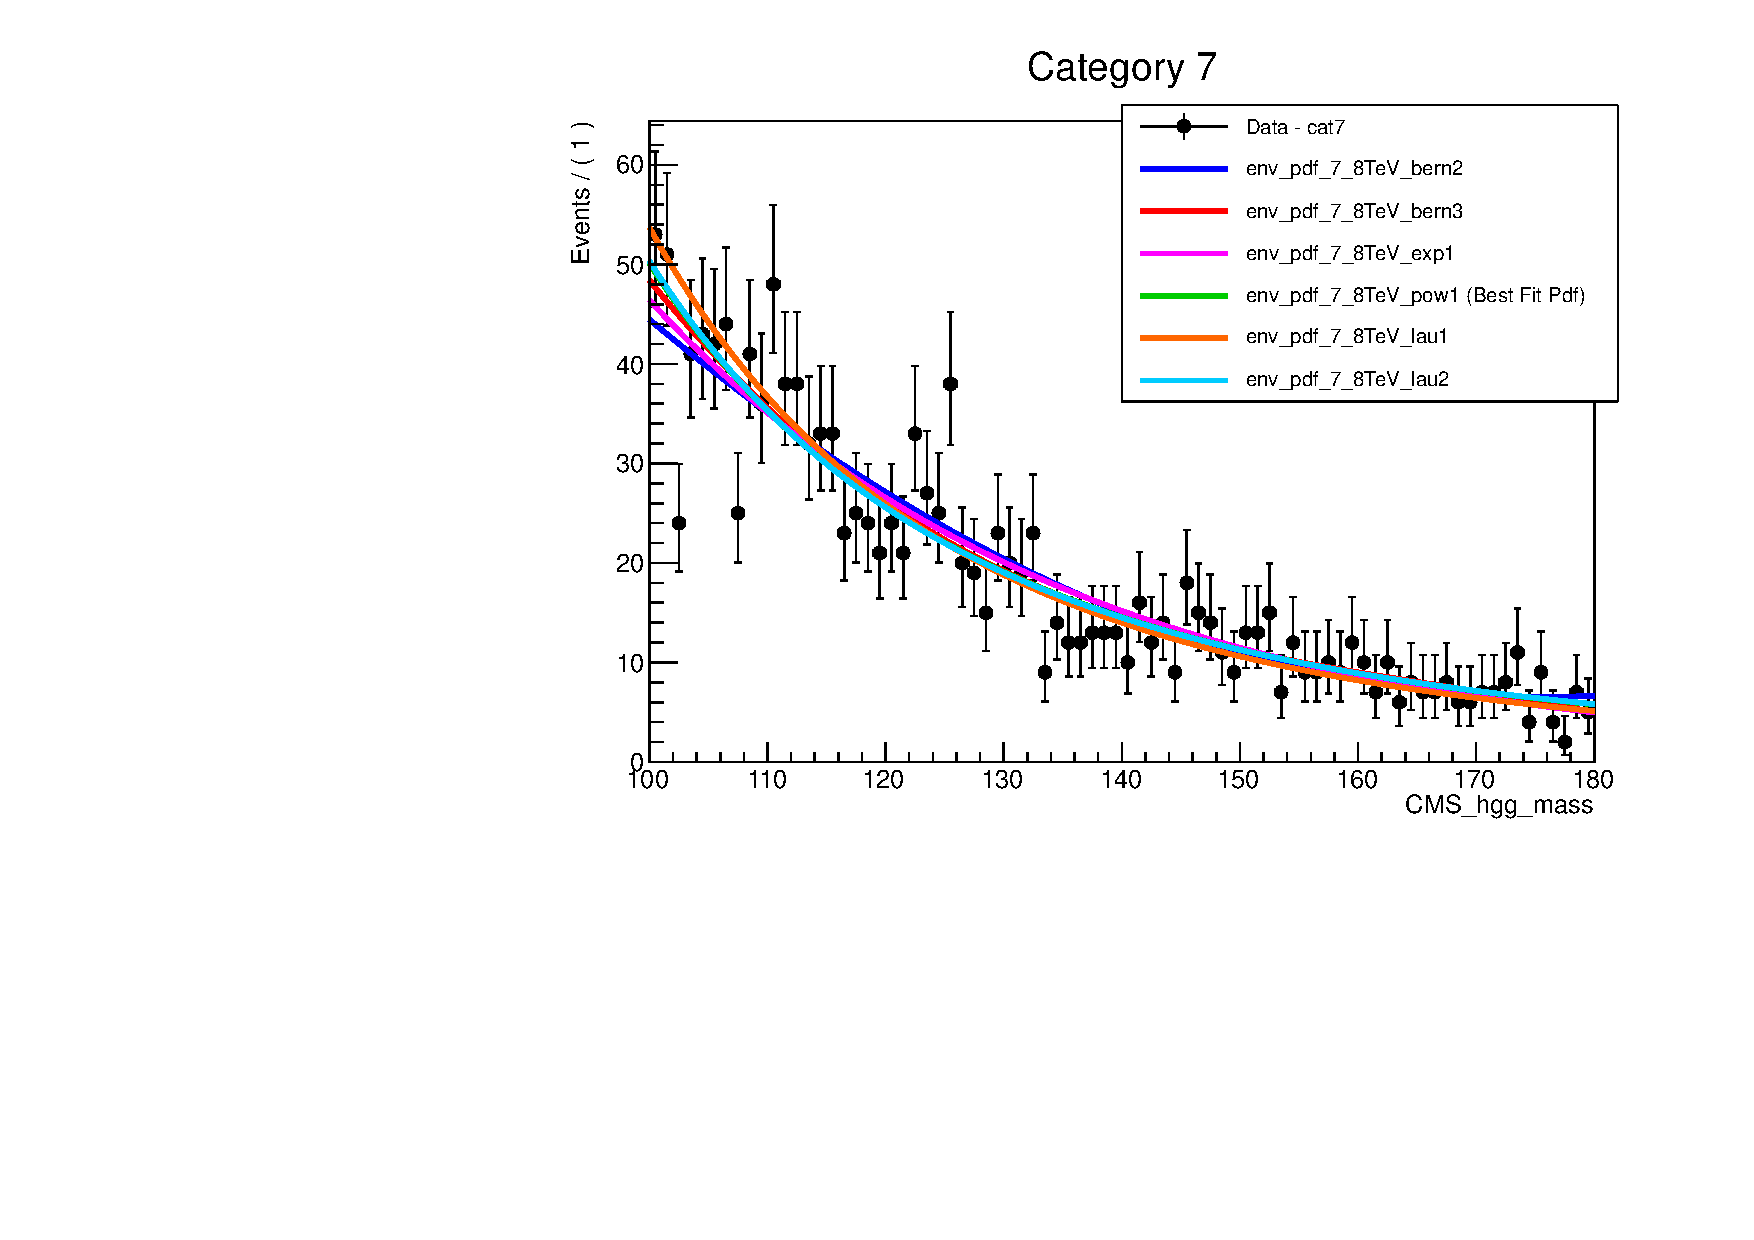
\includegraphics[width=0.49\textwidth]{ch5_anal_and_results/plots/mva_8TeV/multipdf_cat7.pdf}
  \caption{The diphoton invariant mass distribution and the function choices for the background envelope for the dijet categories in the 8~\TeV dataset. \red{Category labels not numbers?}}
  \label{fig:multipdf5}
\end{figure}

\begin{figure}
  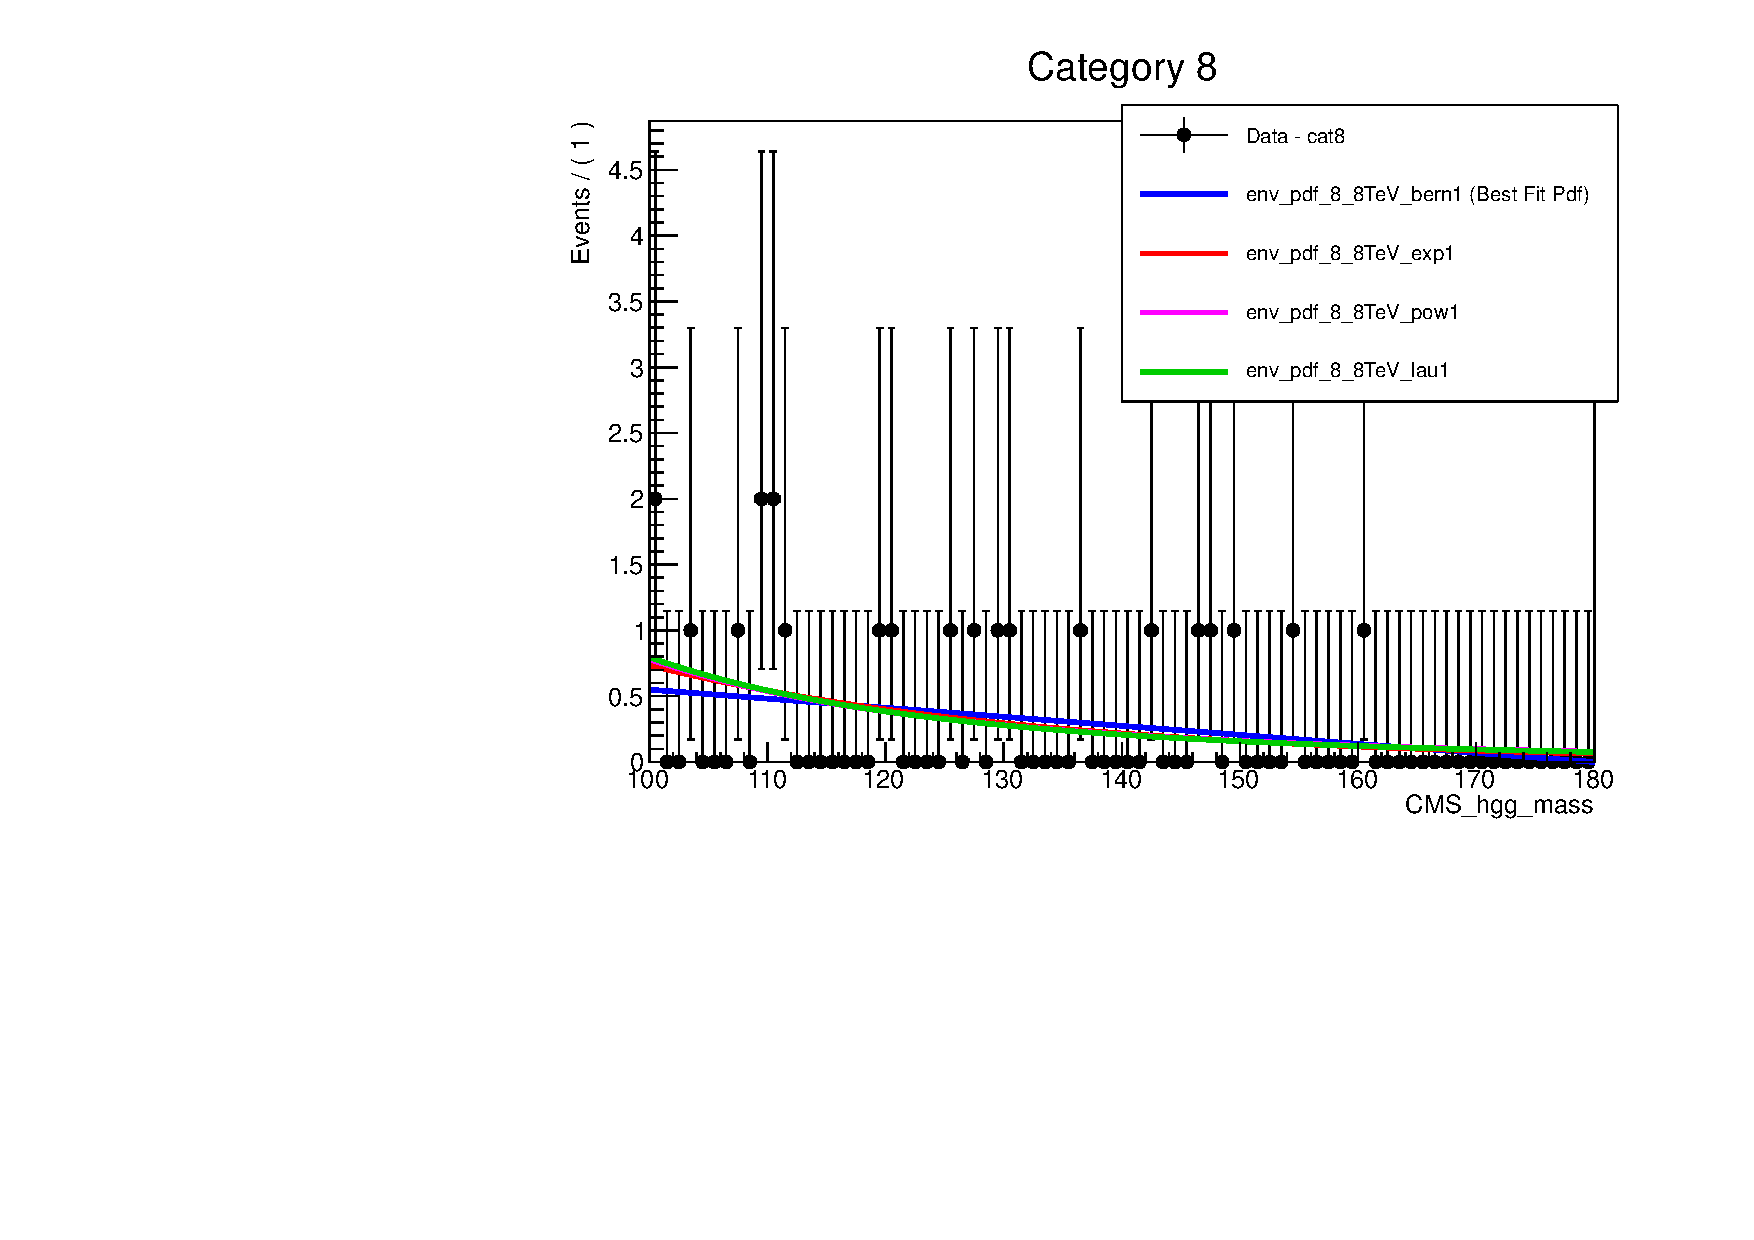
\includegraphics[width=0.49\textwidth]{ch5_anal_and_results/plots/mva_8TeV/multipdf_cat8.pdf}
  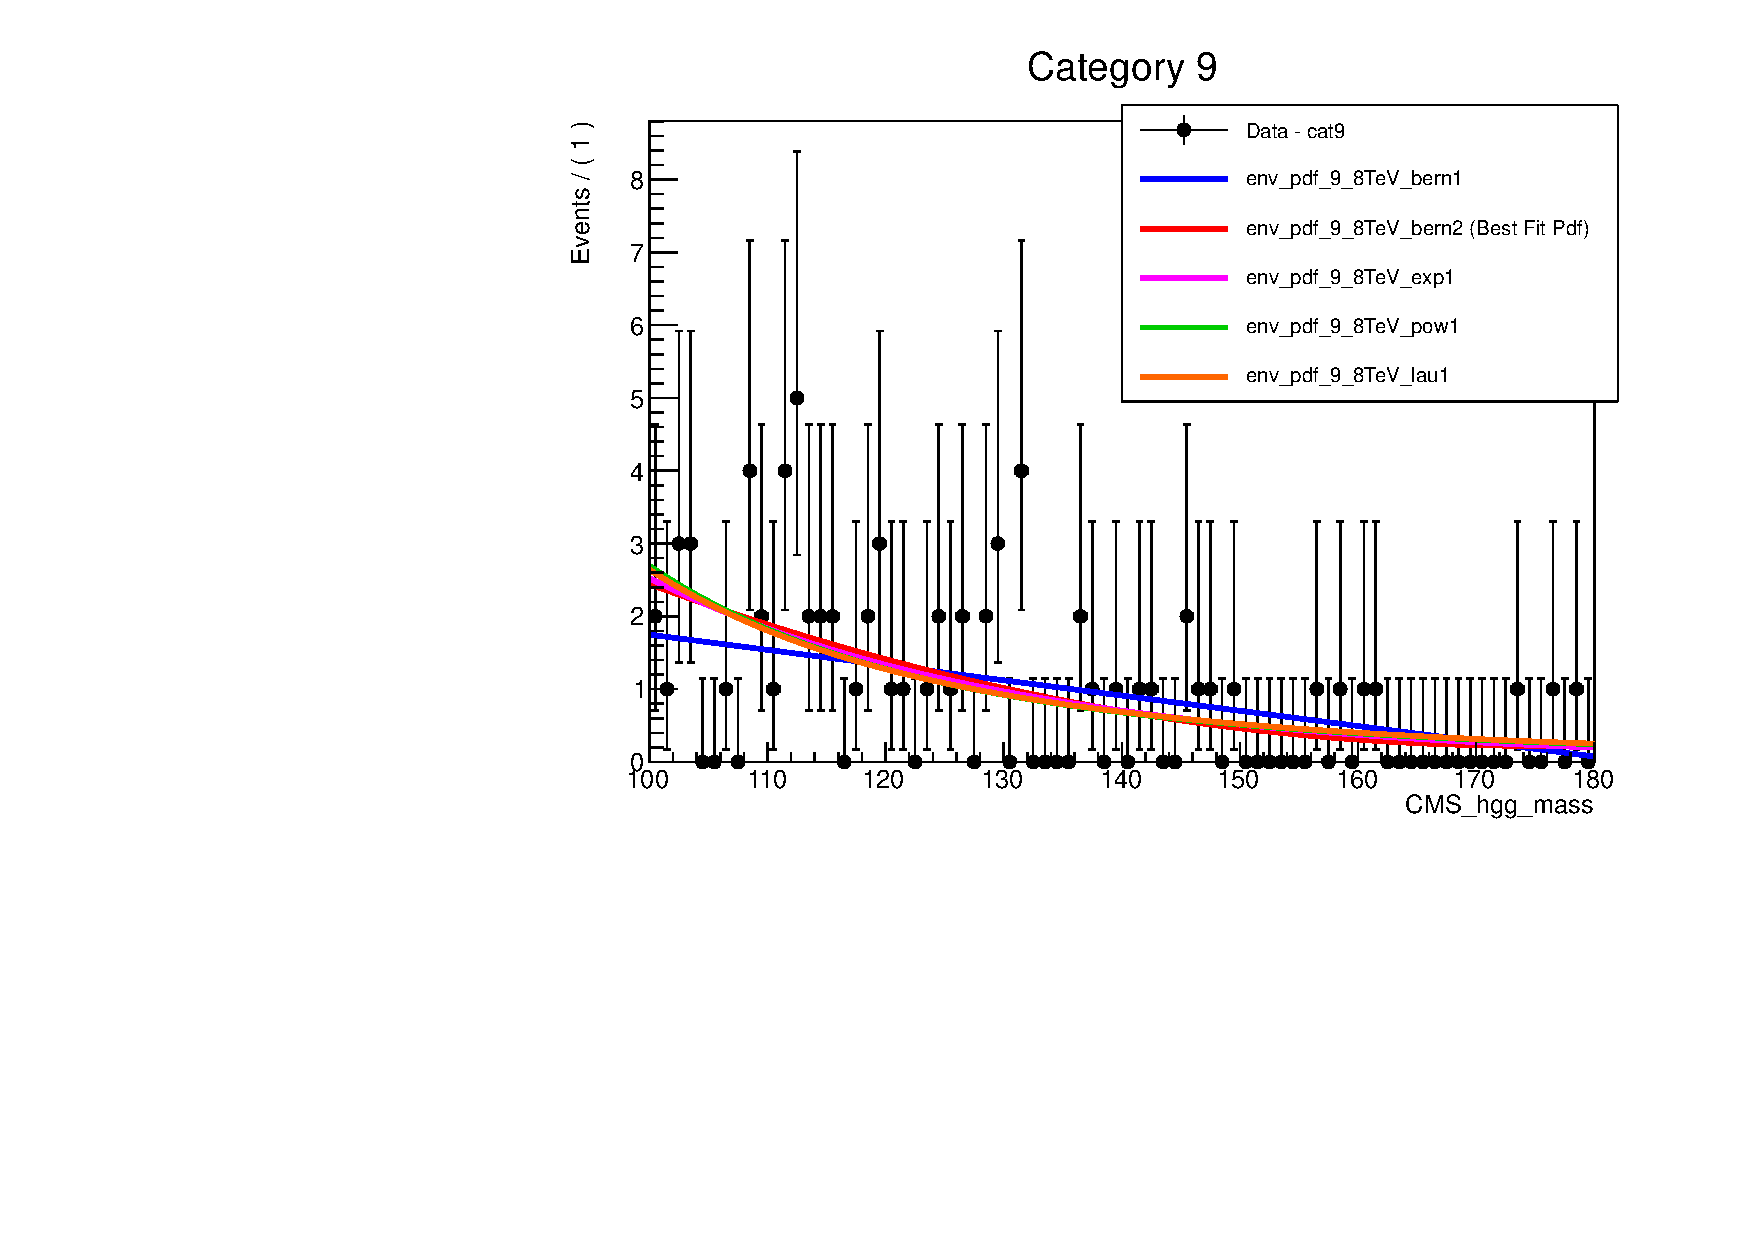
\includegraphics[width=0.49\textwidth]{ch5_anal_and_results/plots/mva_8TeV/multipdf_cat9.pdf}\\
  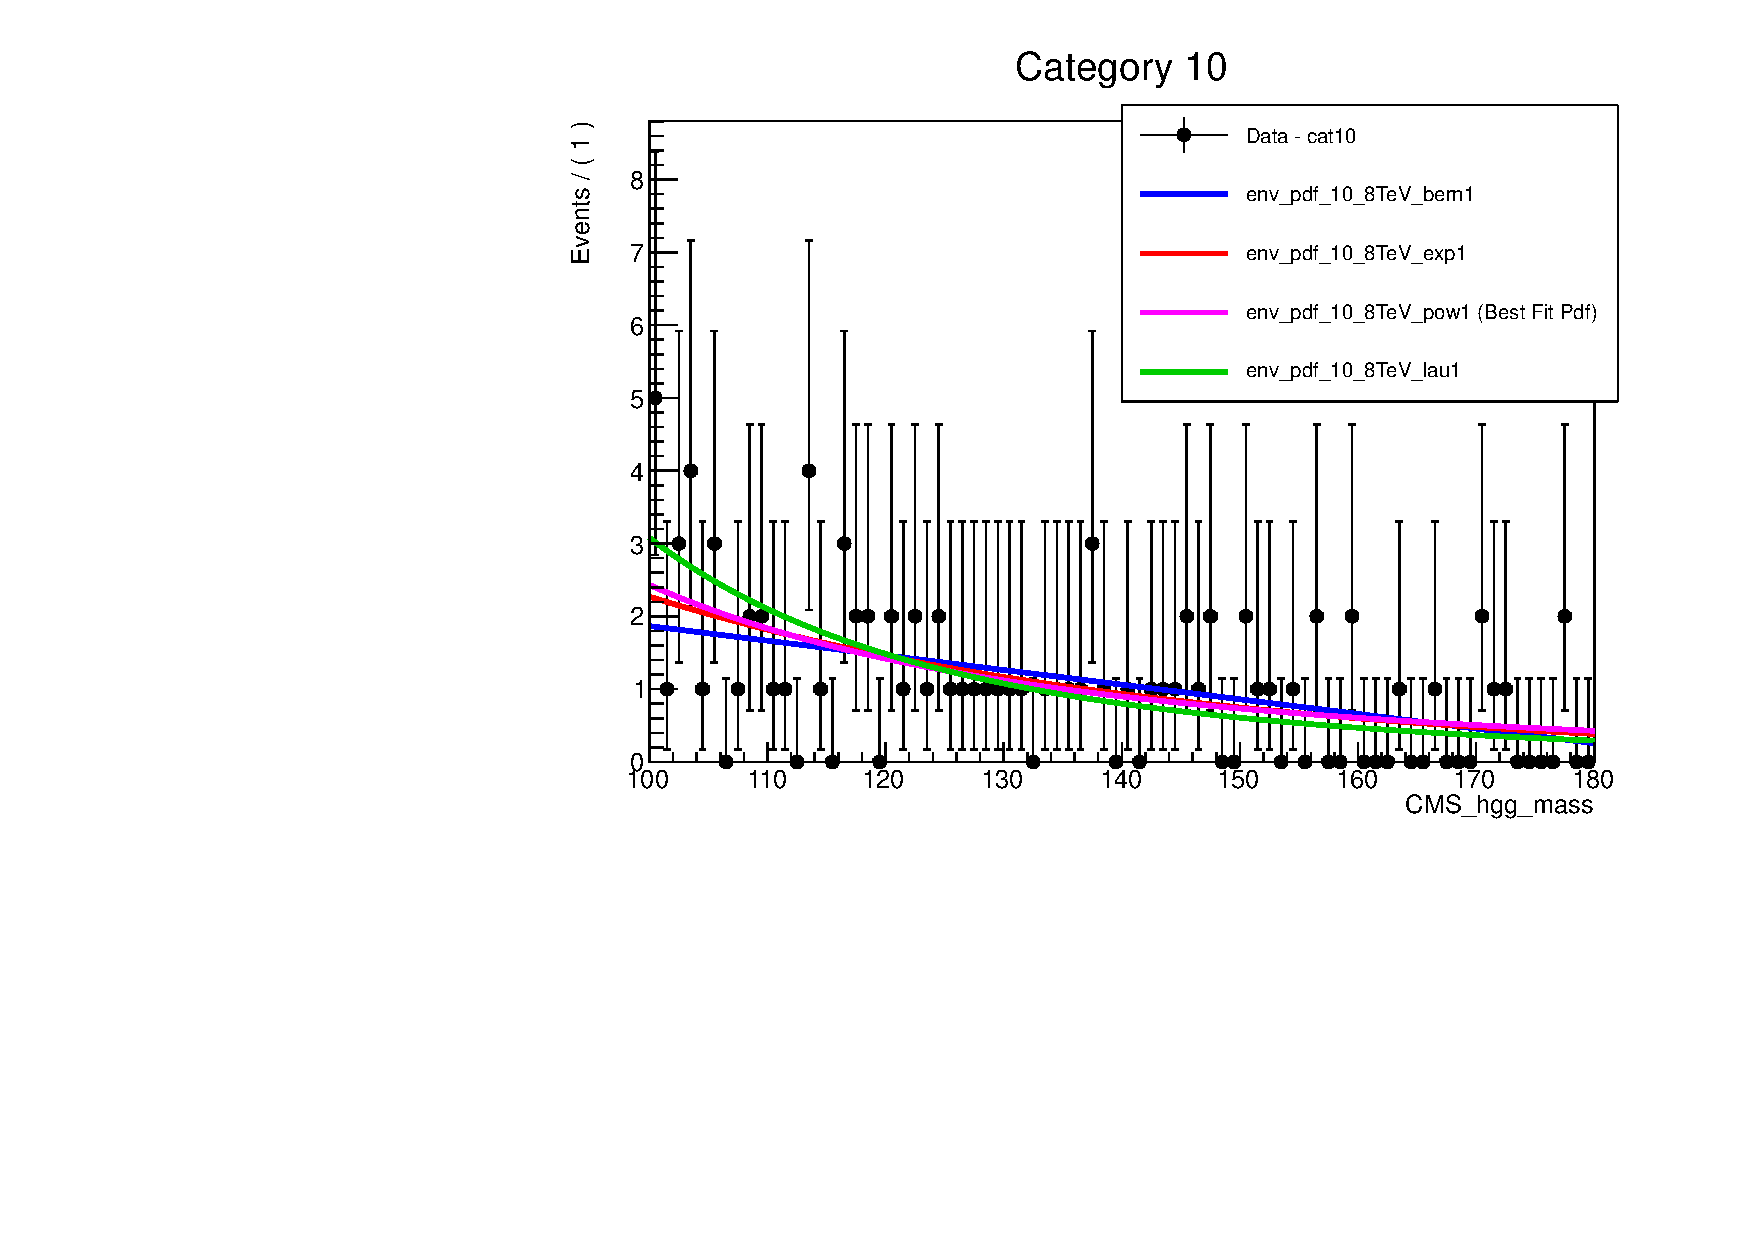
\includegraphics[width=0.49\textwidth]{ch5_anal_and_results/plots/mva_8TeV/multipdf_cat10.pdf}
  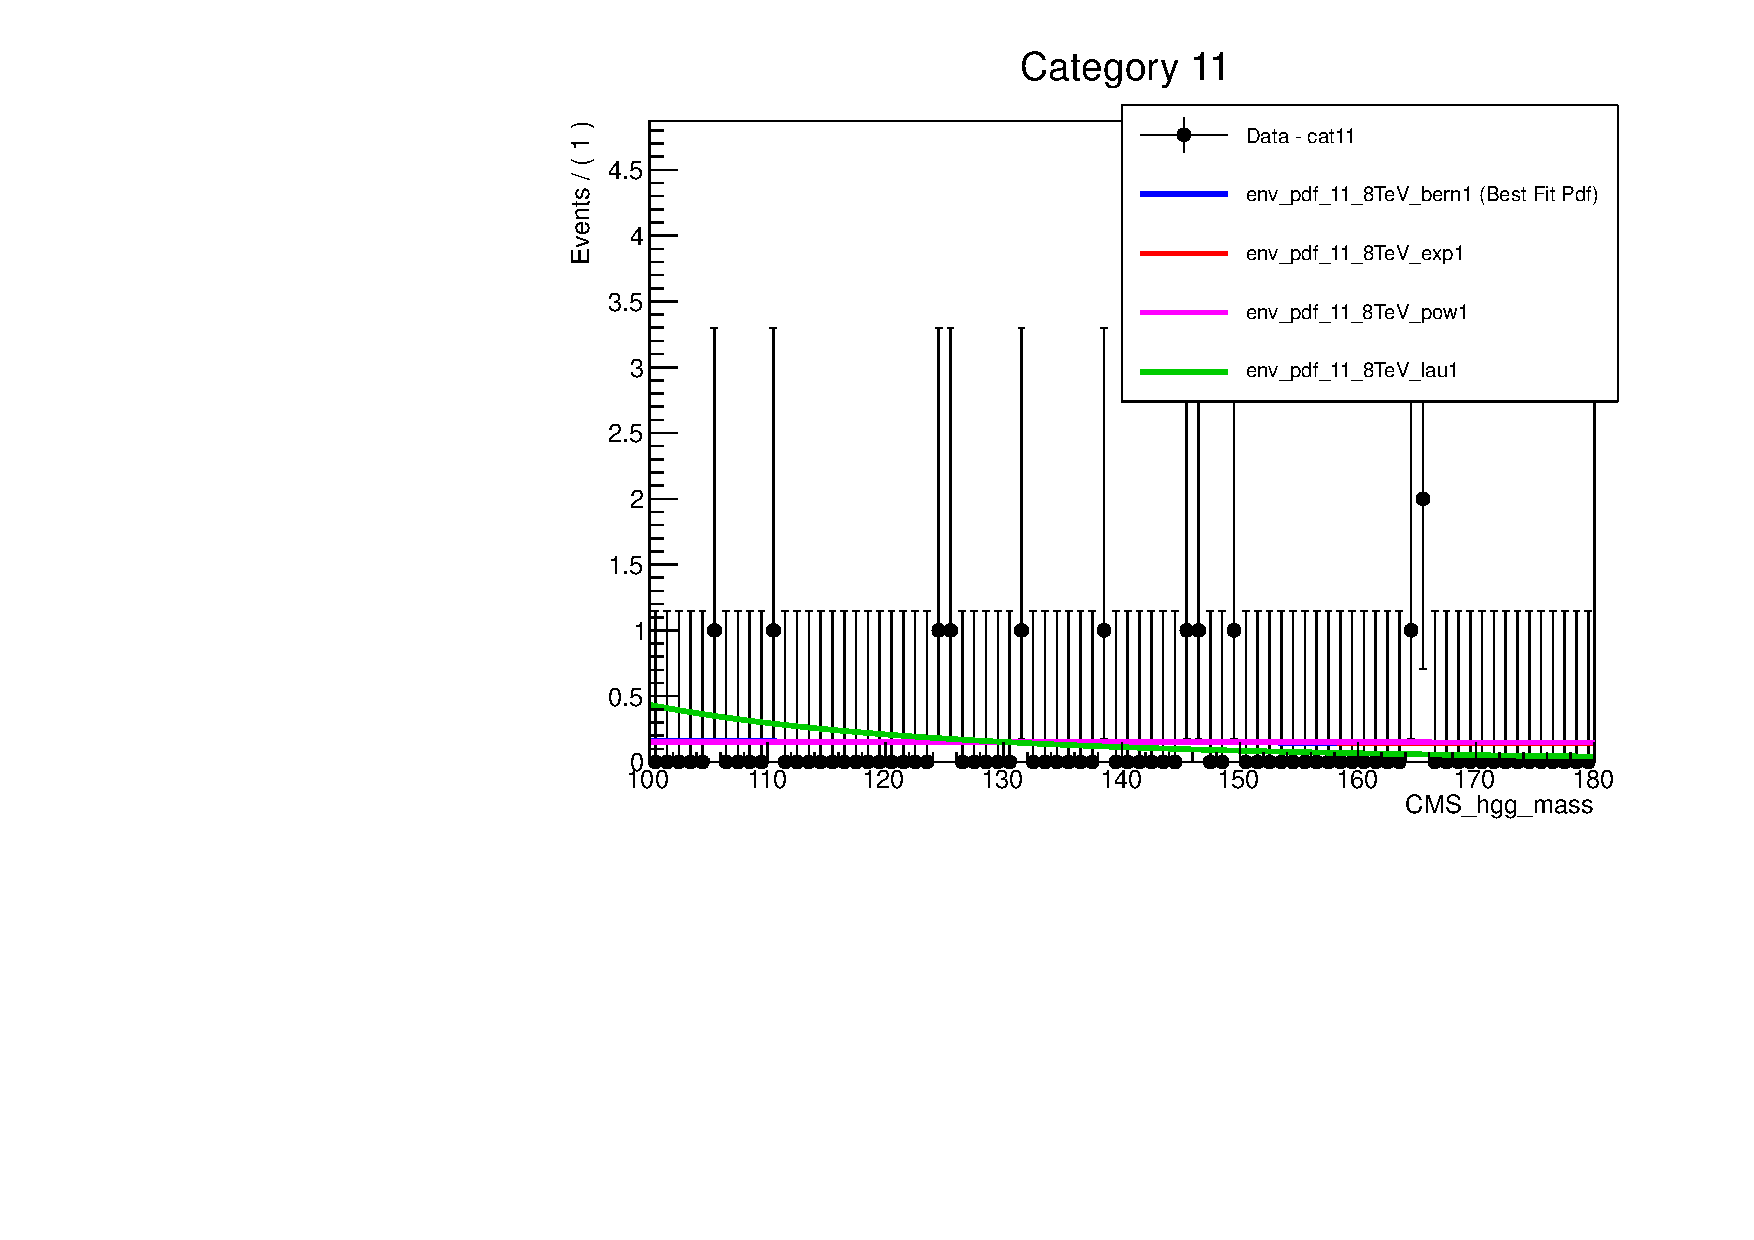
\includegraphics[width=0.49\textwidth]{ch5_anal_and_results/plots/mva_8TeV/multipdf_cat11.pdf}\\
  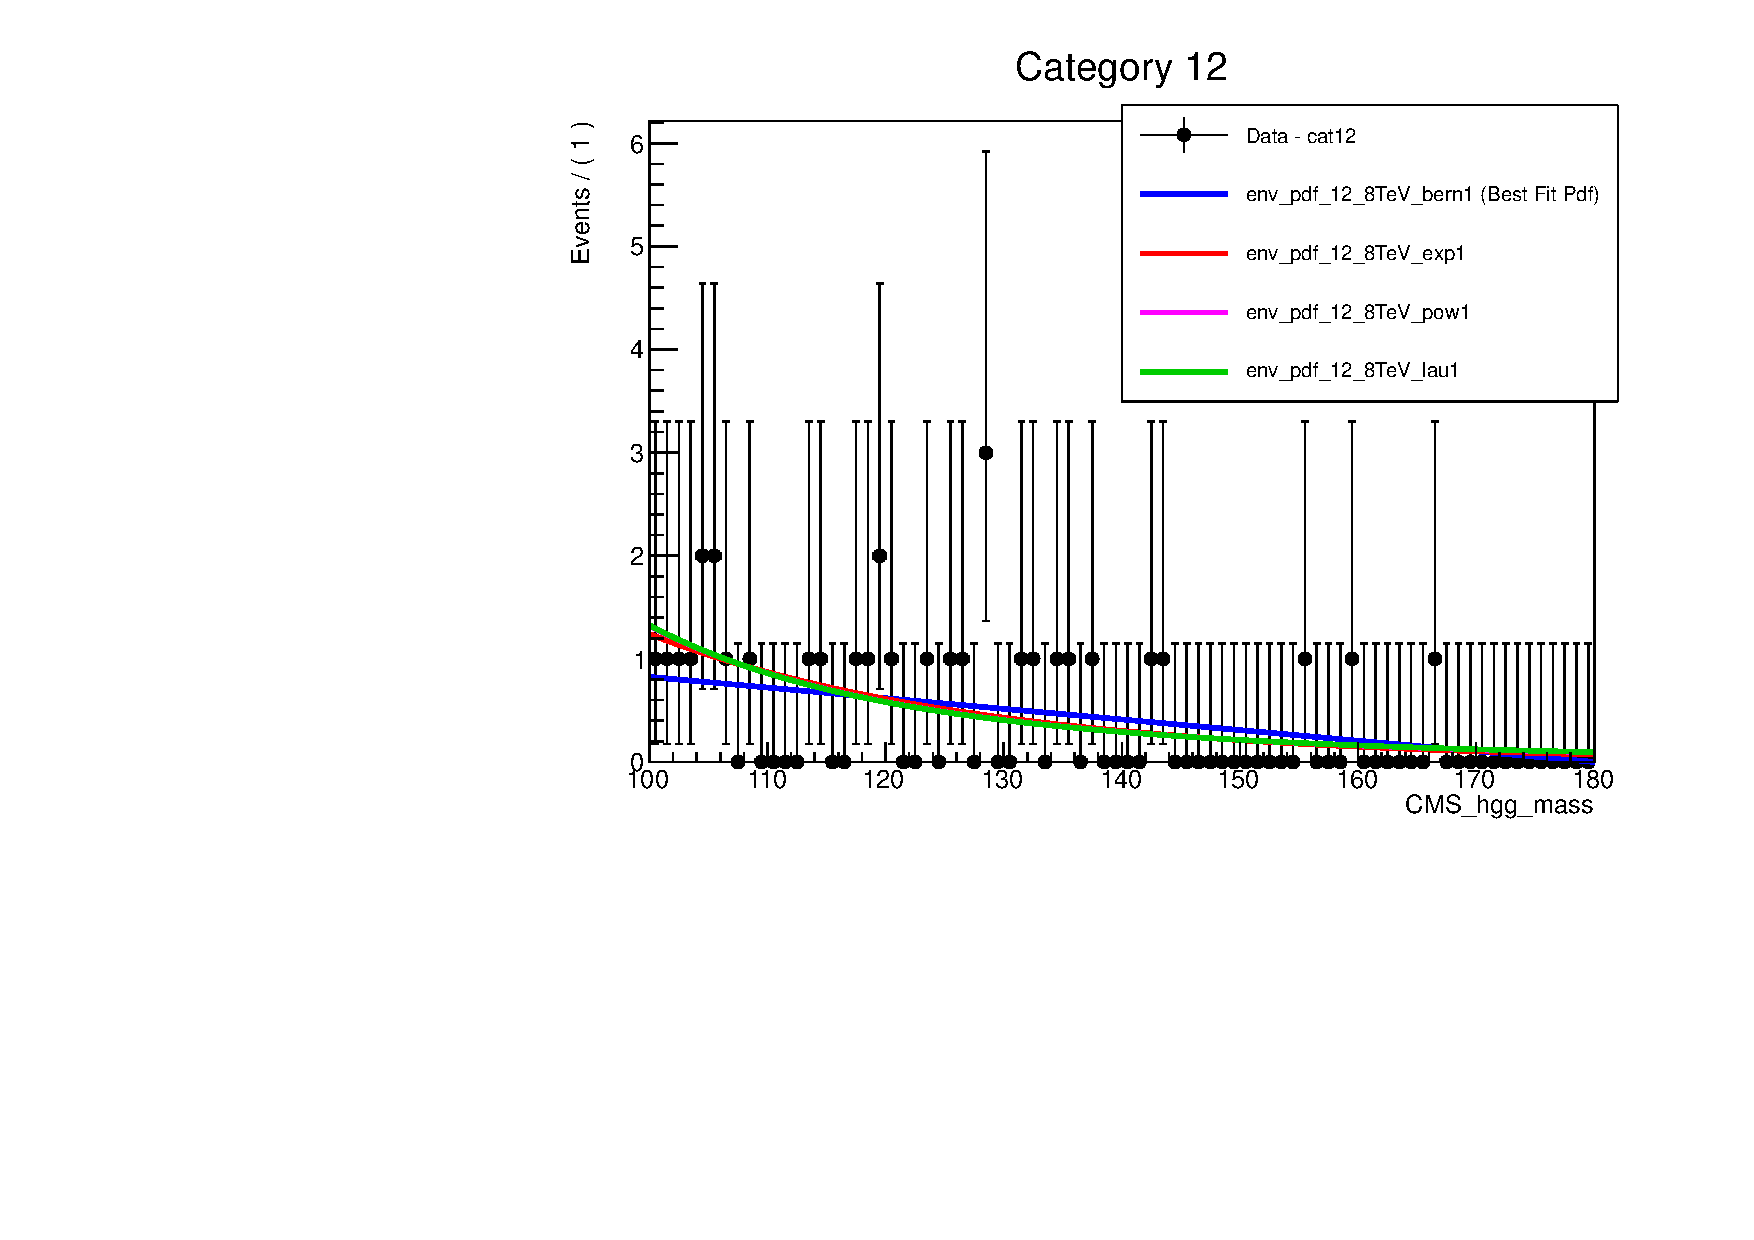
\includegraphics[width=0.49\textwidth]{ch5_anal_and_results/plots/mva_8TeV/multipdf_cat12.pdf}
  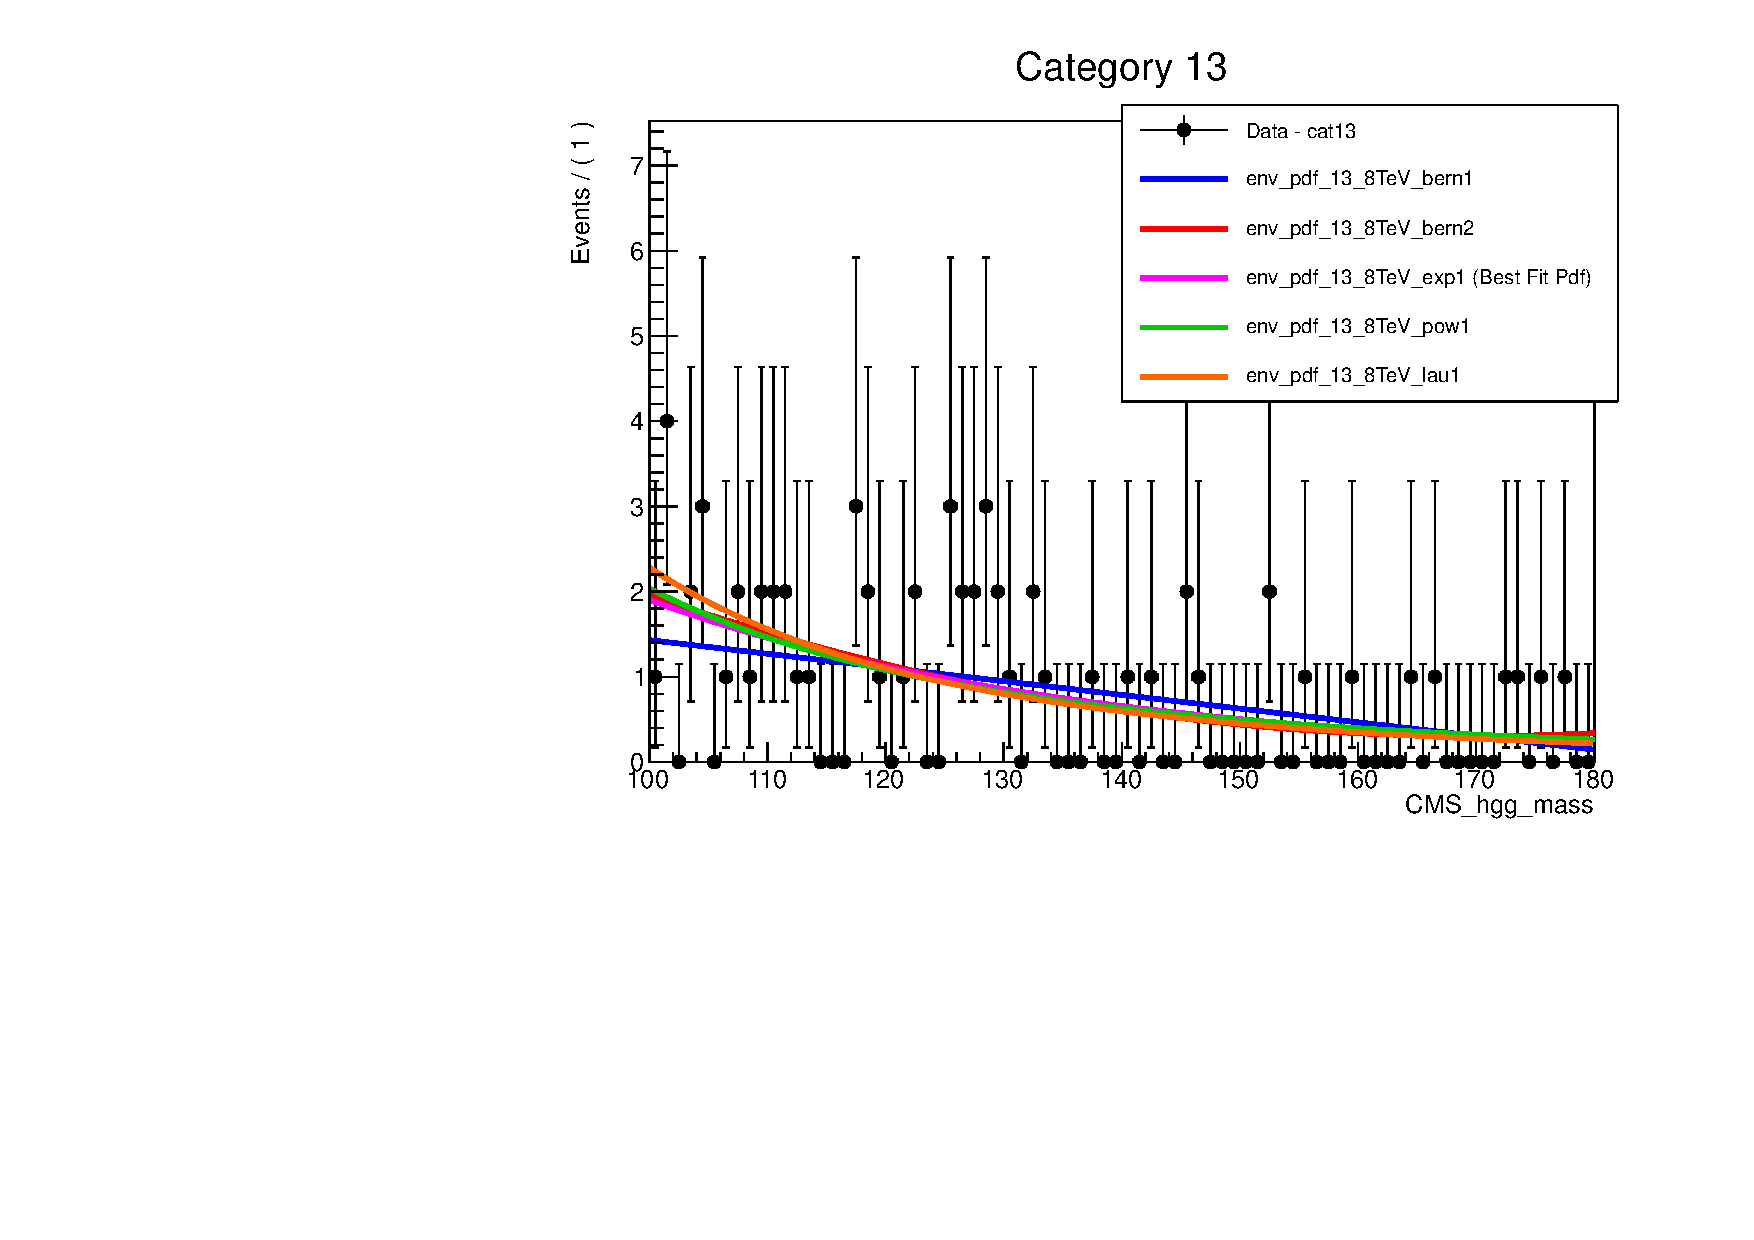
\includegraphics[width=0.49\textwidth]{ch5_anal_and_results/plots/mva_8TeV/multipdf_cat13.pdf}\\
  \caption{The diphoton invariant mass distribution and the function choices for the background envelope for the \VH and \ttH categories in the 8~\TeV dataset. \red{Category labels not numbers?}}
  \label{fig:multipdf6}
\end{figure}

\subsection{Sideband analysis}

In the sideband analysis the shape and normalisation of the background are obtained separately. The overall normalisation is extracted from a parametric fit of the entire invariant mass distribution excluding the $\pm$2\% signal window. The shape, which is to say the distribution of events in each analysis bin, is extracted from invariant mass sidebands. Each sideband is defined to have the equivalent width of $\pm$2\% relative to the invariant mass that corresponds to the centre of the sideband. For a \SM Higgs at 125~\GeV about 75\% of the signal is contained within the window. Consequently a sideband either side of the signal window is skipped and then three sidebands on either side of the hypothesised mass in question are used. Figure~\ref{fig:sideband_norm} shows the inclusive invariant mass distribution for the 8~\TeV dataset, the parametric function used to extract the normalisation of events in the window, the signal region (in red) and the six sidebands (in blue).

In order to avoid Drell-Yan contamination in the region of low invariant mass any sideband whose lower boundary is less than 100~\GeV is removed and an additional sideband is added to the high side of the signal region. Consequently any mass hypothesis in the range $111\leq\mH< 115.5$ has two lower and four upper sidebands and any mass hypothesis in the range $100\leq\mH<111$ has one lower and five upper sidebands.

\begin{figure}
  \begin{center}
    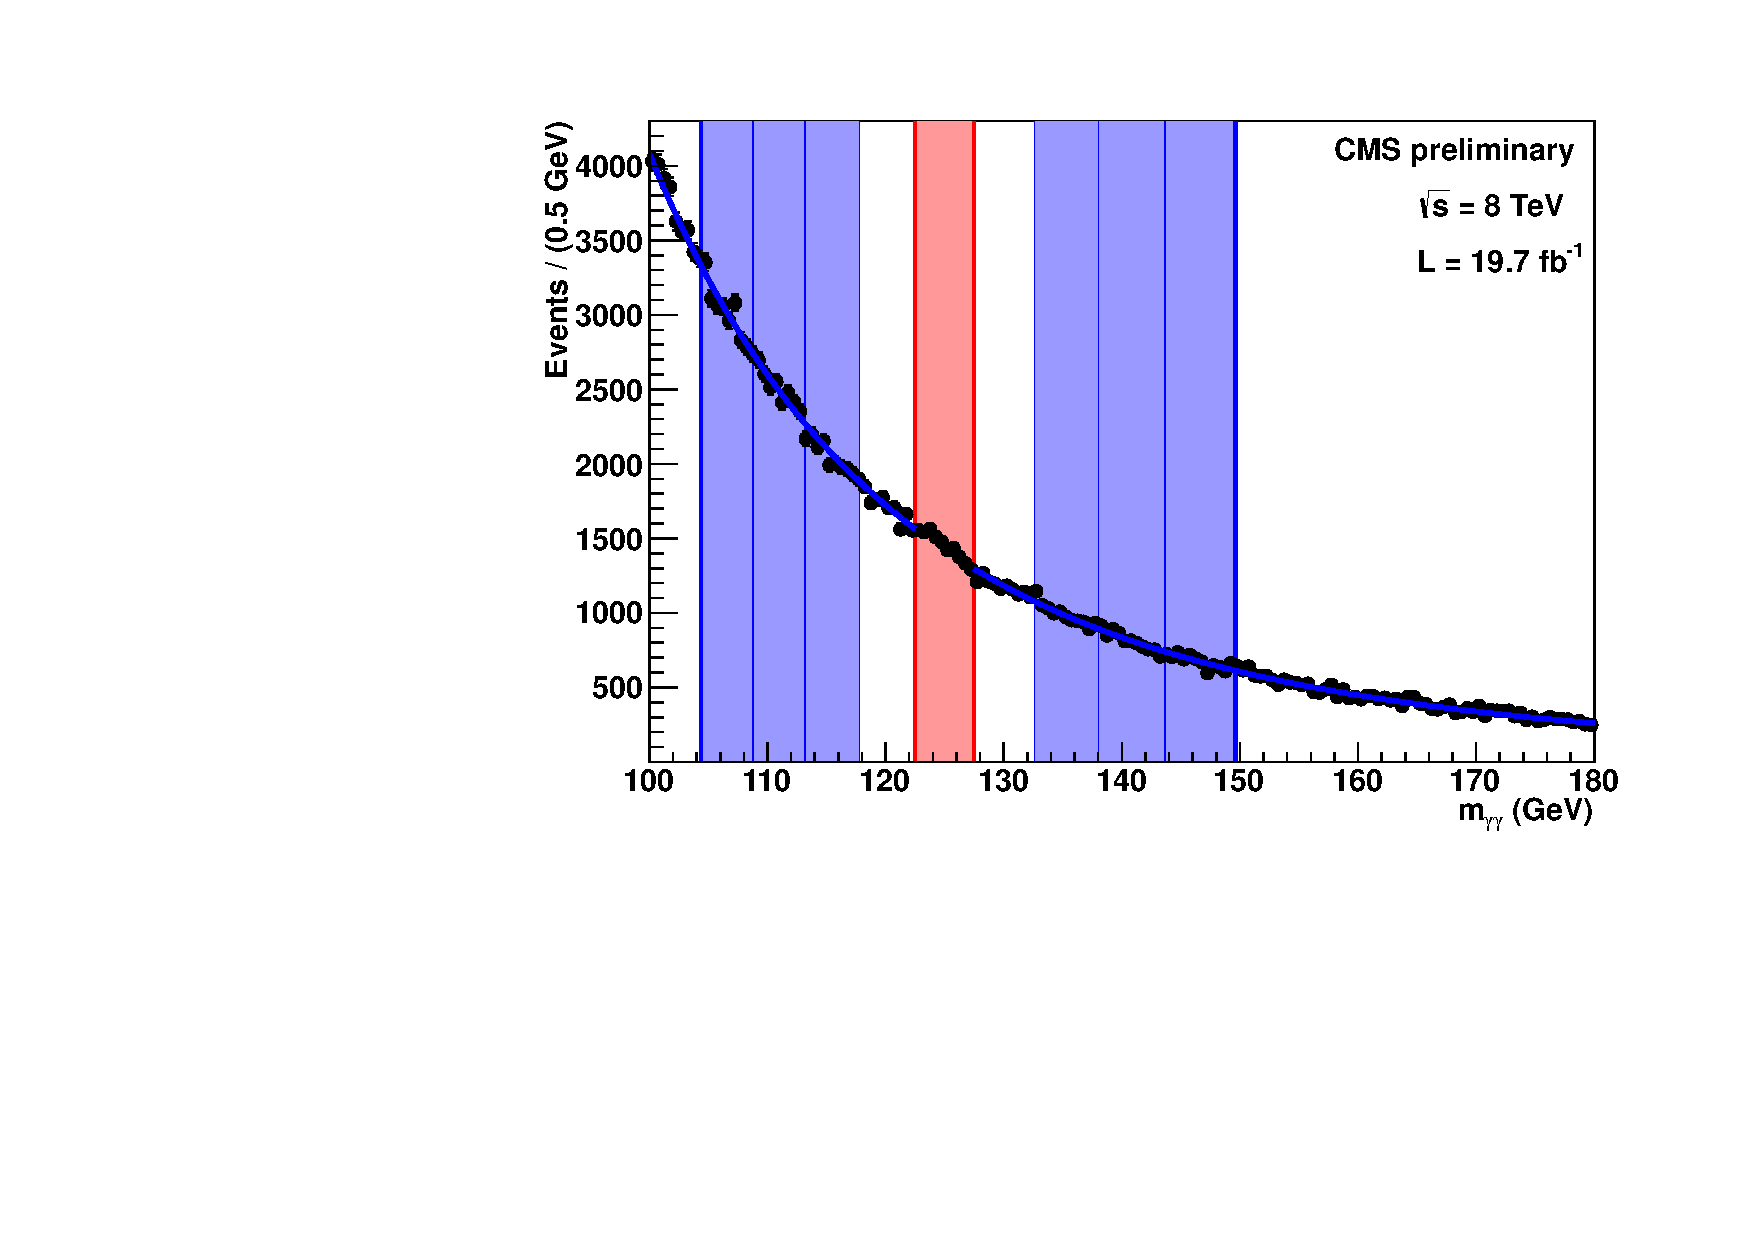
\includegraphics[width=0.85\textwidth]{ch5_anal_and_results/plots/sideband/invmass.pdf}
    \caption{The inclusive invariant mass distribution for the 8TeV dataset in data (black points). An illustration of the signal region (red) and the sidebands (blue) used for the mass hypothesis \mH=125~\GeV is shown. The parametric function used to obtain the normalisation in the signal region is shown as the blue line.}
    \label{fig:sideband_norm}
  \end{center}
\end{figure}

The parametric form used to obtain the normalisation is a single term power law (one degree of freedom) for the 8~\TeV dataset and a two term Laurent series (one degree of freedom) for the 7~\TeV dataset. The functions are defined identically to those described for the envelope method in Sec.~\ref{sec:envelope}. These functions are chosen because they give the smallest uncertainty when accounting for biases incurred by picking the wrong functional form. A systematic uncertainty is applied to the normalisation term of which there are more details later in Sec.~\ref{sec:systematics}.

The estimated number of background events in the signal region is obtained from the data in the sidebands. It is assumed that the fraction of events in each bin varies linearly with invariant mass (i.e.~across sidebands) and that there is negligble signal contamination in the sidebands. For each bin, $b$, the fraction of events for a given mass is taken to be,

\begin{equation}
  f_{b} = p_{0b} + p_{1b}(m-m_{H}),
\end{equation}

where $p_{0b}$ and $p_{1b}$ are the Taylor expansion coefficients for bin $b$. Since the fractions must sum to unity for any given mass (the noramlisation is extracted elsewhere) then for $N$ bins there are $2(N-1)$ coefficiets. These coefficients are determined by fitting a straight line across the sidebands in each bin, with the constraint that the fraction in each sideband must sum to 1 across all the bins. An example of ones of these fits is shown in Fig.~\ref{fig:sideband_shape}.

\begin{figure}
  \begin{center}
    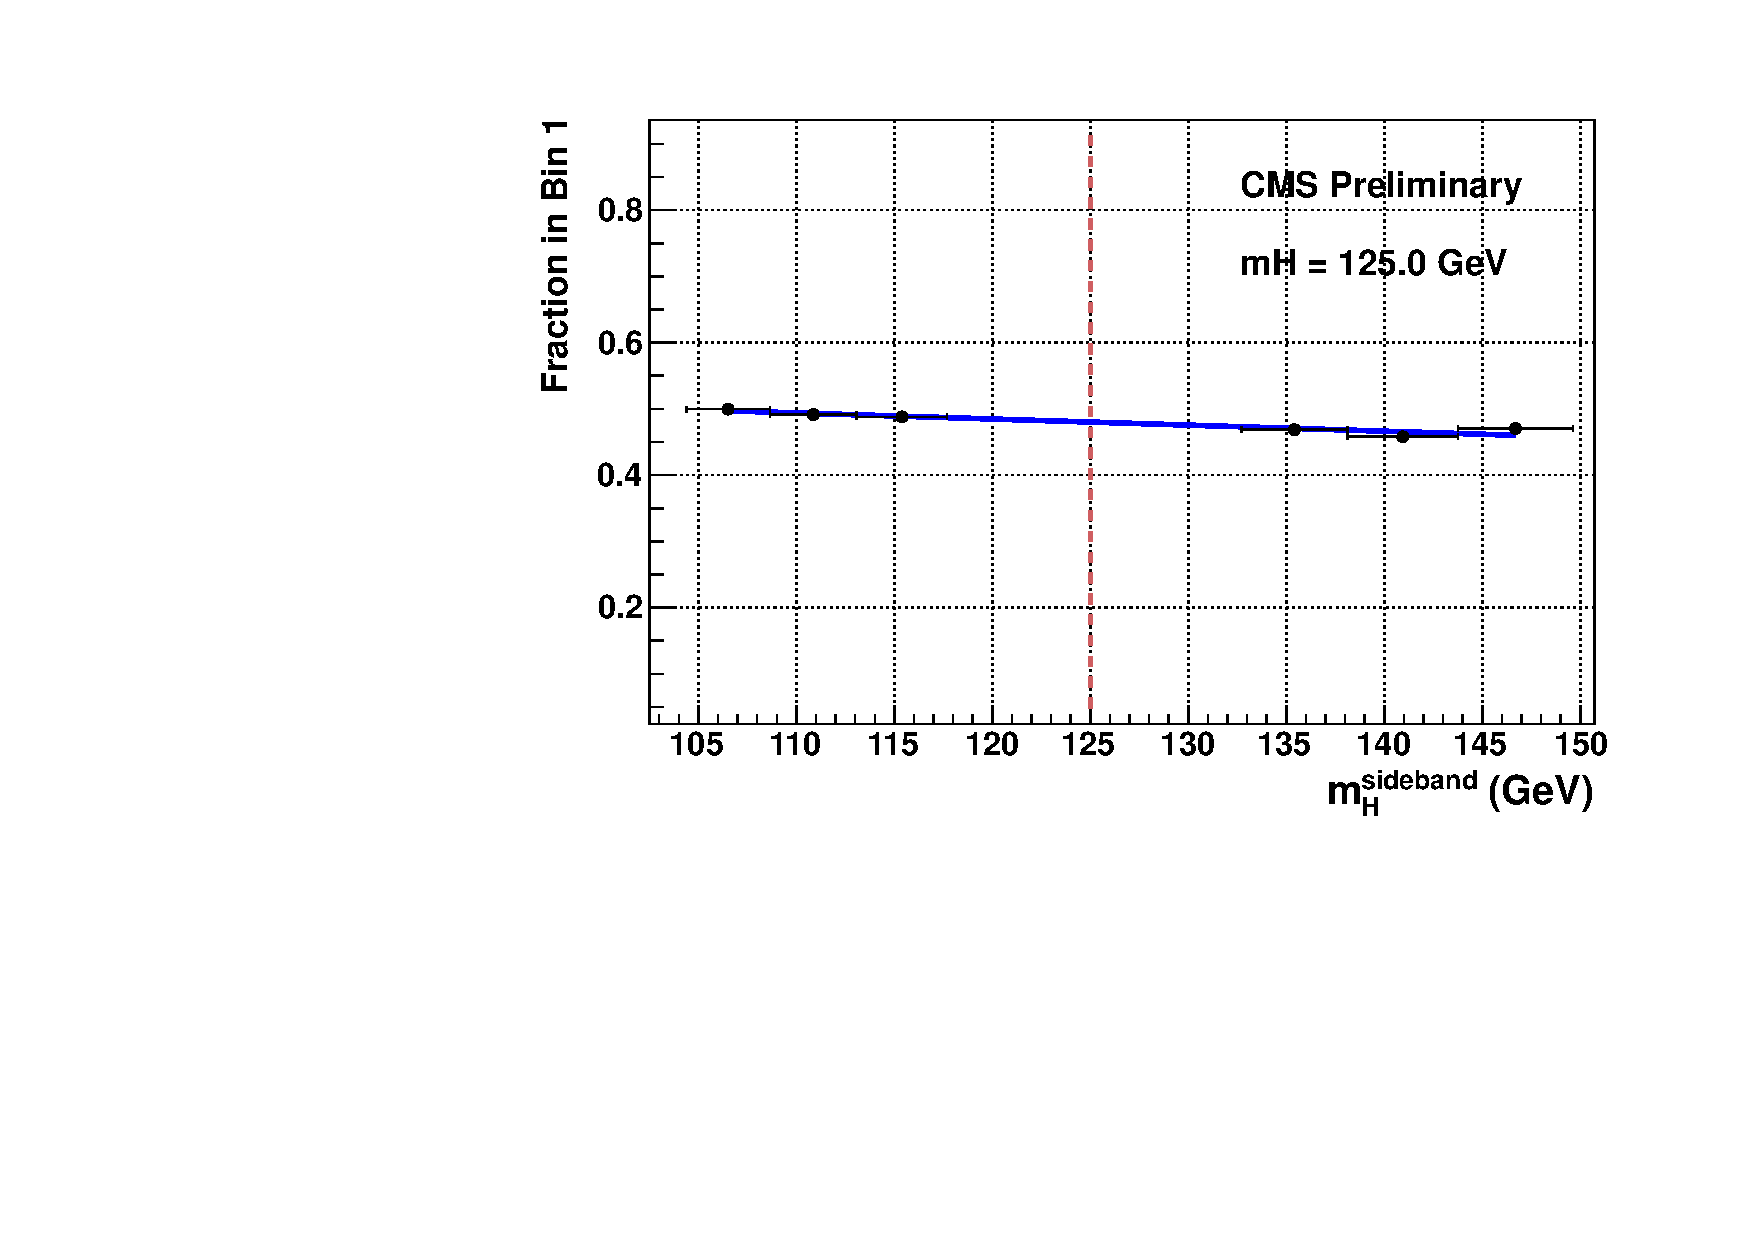
\includegraphics[width=0.85\textwidth]{ch5_anal_and_results/plots/sideband/sideband_fit.pdf}
    \caption{The number of data events is shown for a single analysis bin in each of the sidebands surrounding the signal window at \mH=125~\GeV (black points). The blue line show the straight line fit for this bin. In the 8~\TeV dataset there are 10 inclusive analysis bins and 9 exclusive analysis bins. Consequently there are 19 of these straight line fits at each \mH but only 18 of them are independent as the fractions must sum to unity.}
    \label{fig:sideband_norm}
  \end{center}
\end{figure}

The distribution for the data, background (along with the $pm1\sigma$ and $\pm2\sigma$ errors) and signal for each of the sideband analysis bins are shown in Figs.~\ref{fig:sideband_output} for the mass hypothesis, \mH=124.7~\GeV.

\begin{figure}
  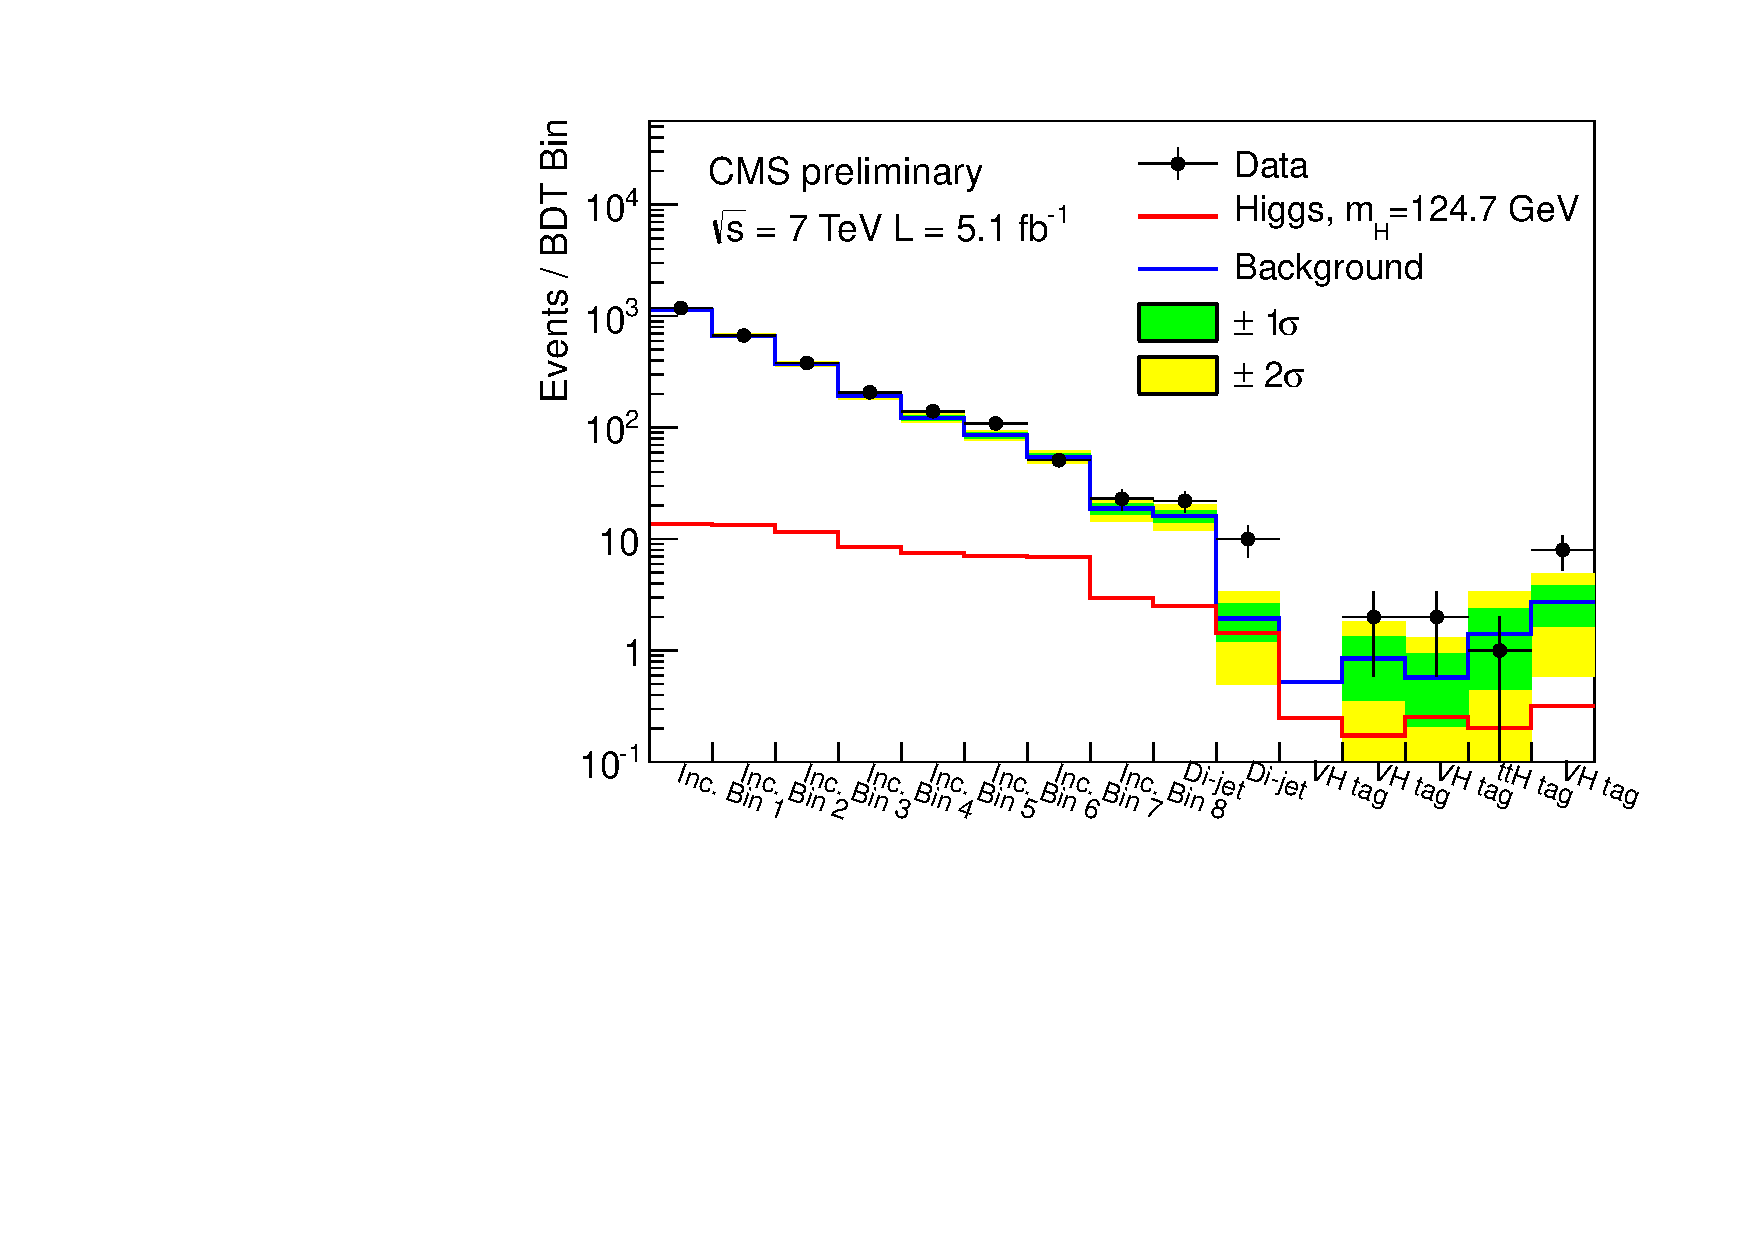
\includegraphics[width=0.48\textwidth]{{ch5_anal_and_results/plots/sideband/model_7TeV_m124.7}.pdf}
  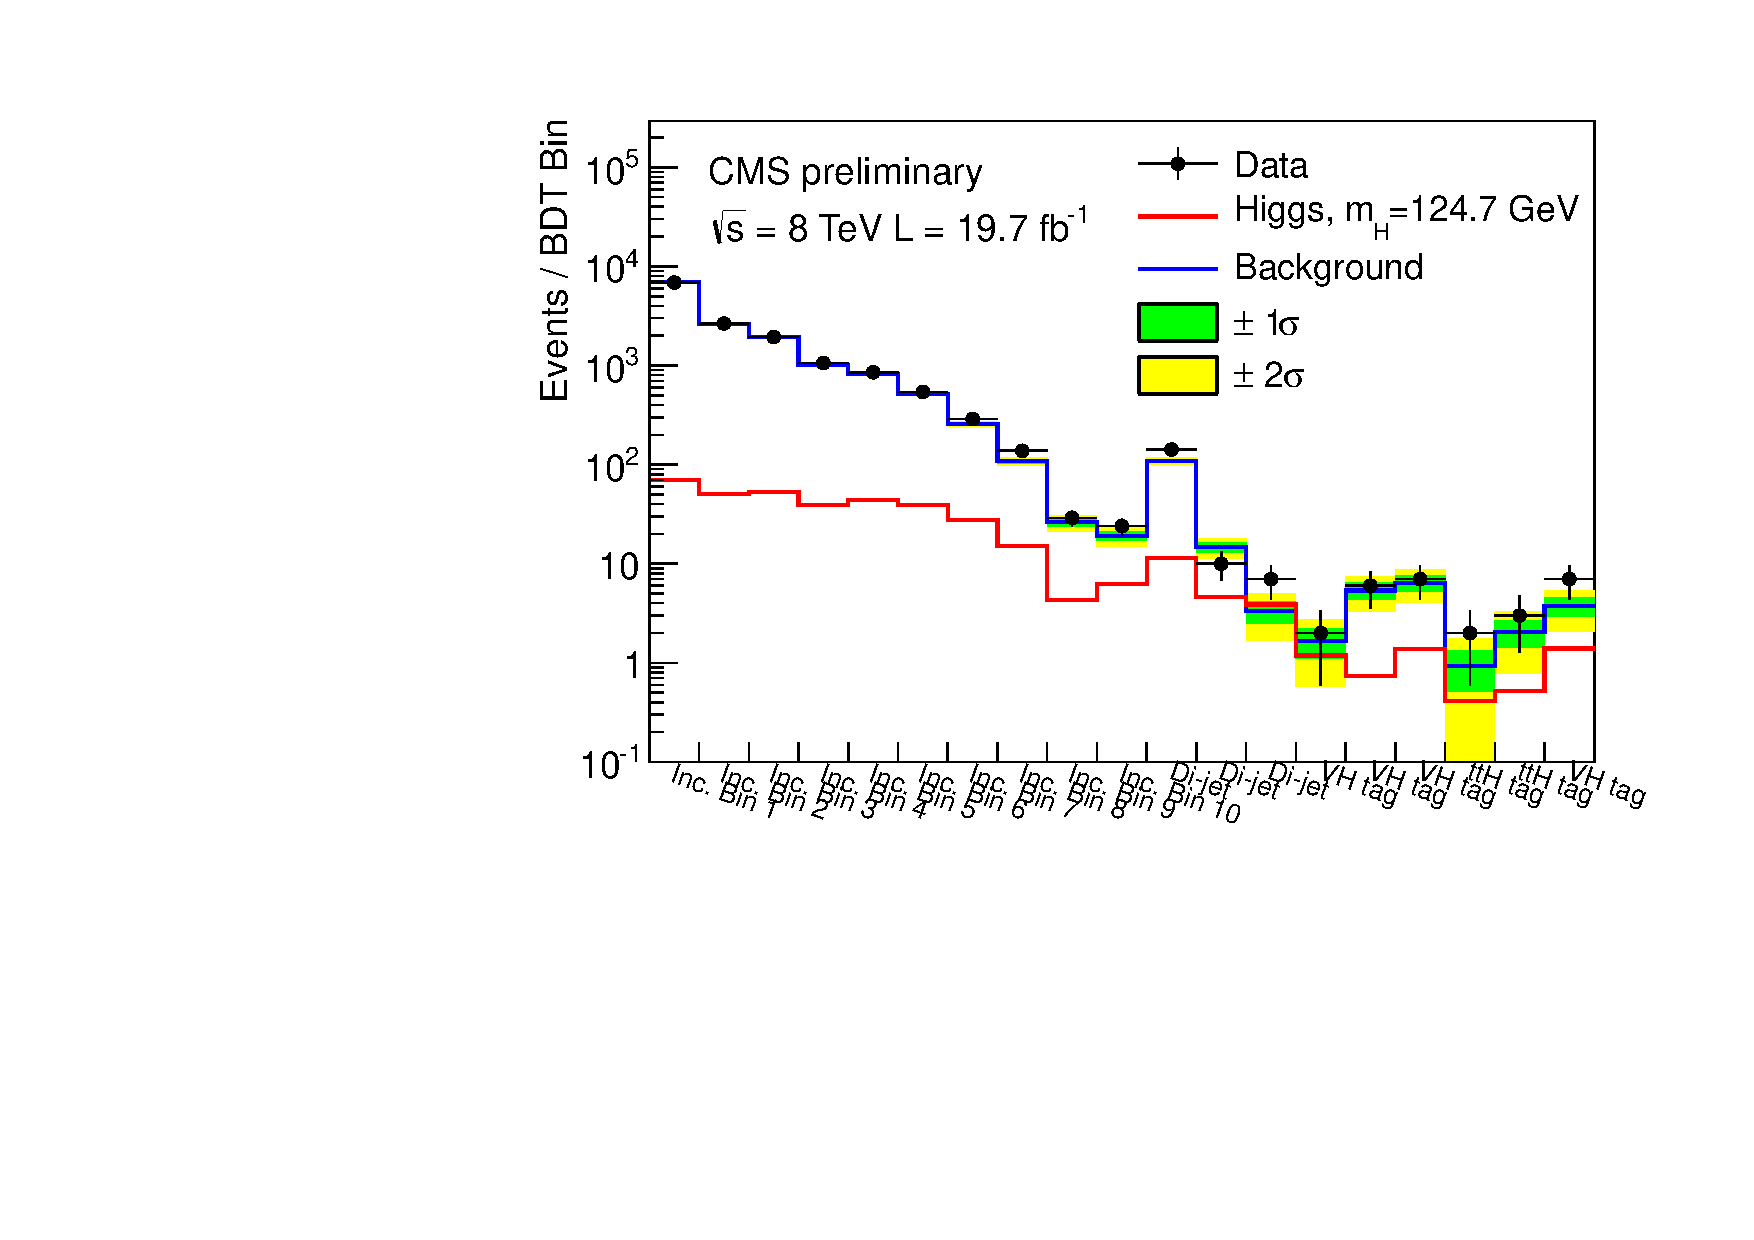
\includegraphics[width=0.48\textwidth]{{ch5_anal_and_results/plots/sideband/model_8TeV_m124.7}.pdf}\\
  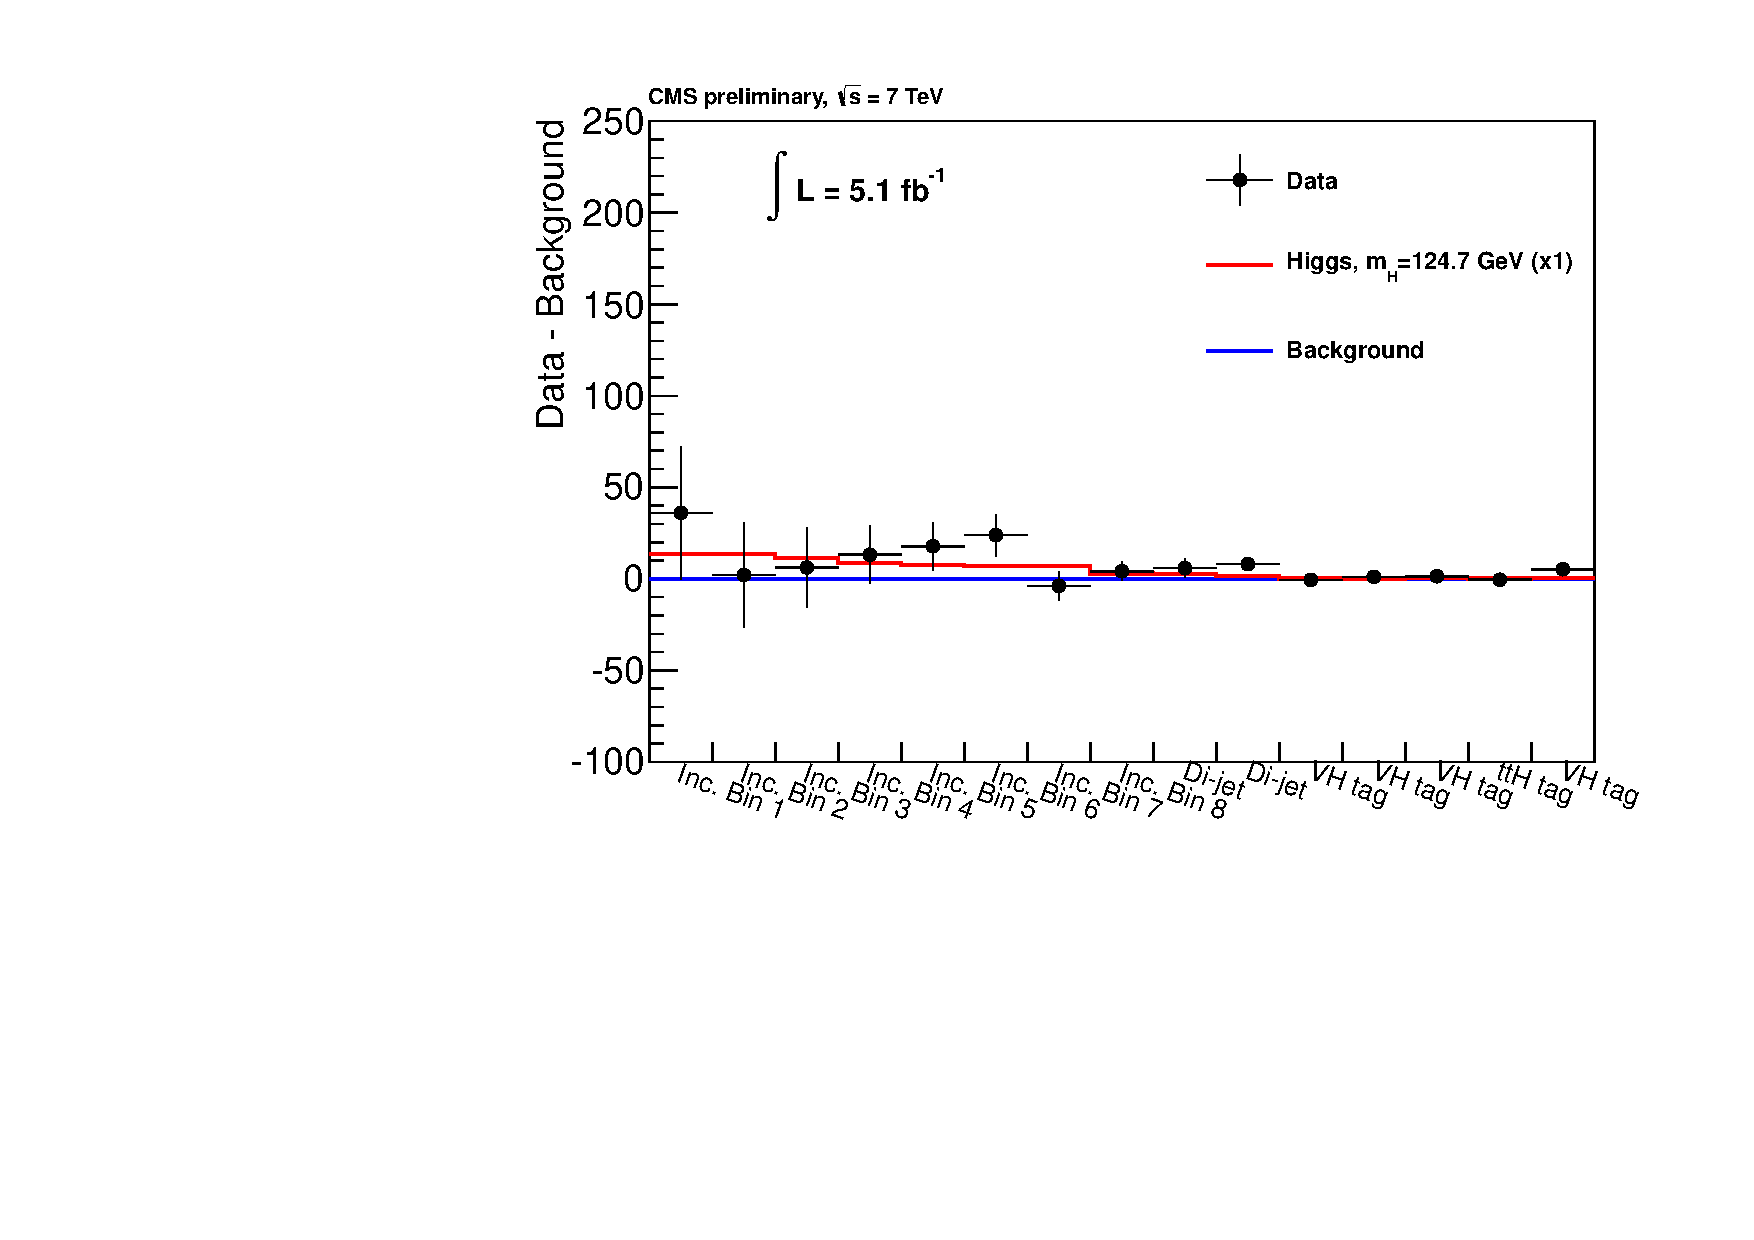
\includegraphics[width=0.48\textwidth]{{ch5_anal_and_results/plots/sideband/diff_model_7TeV_m124.7}.pdf}
  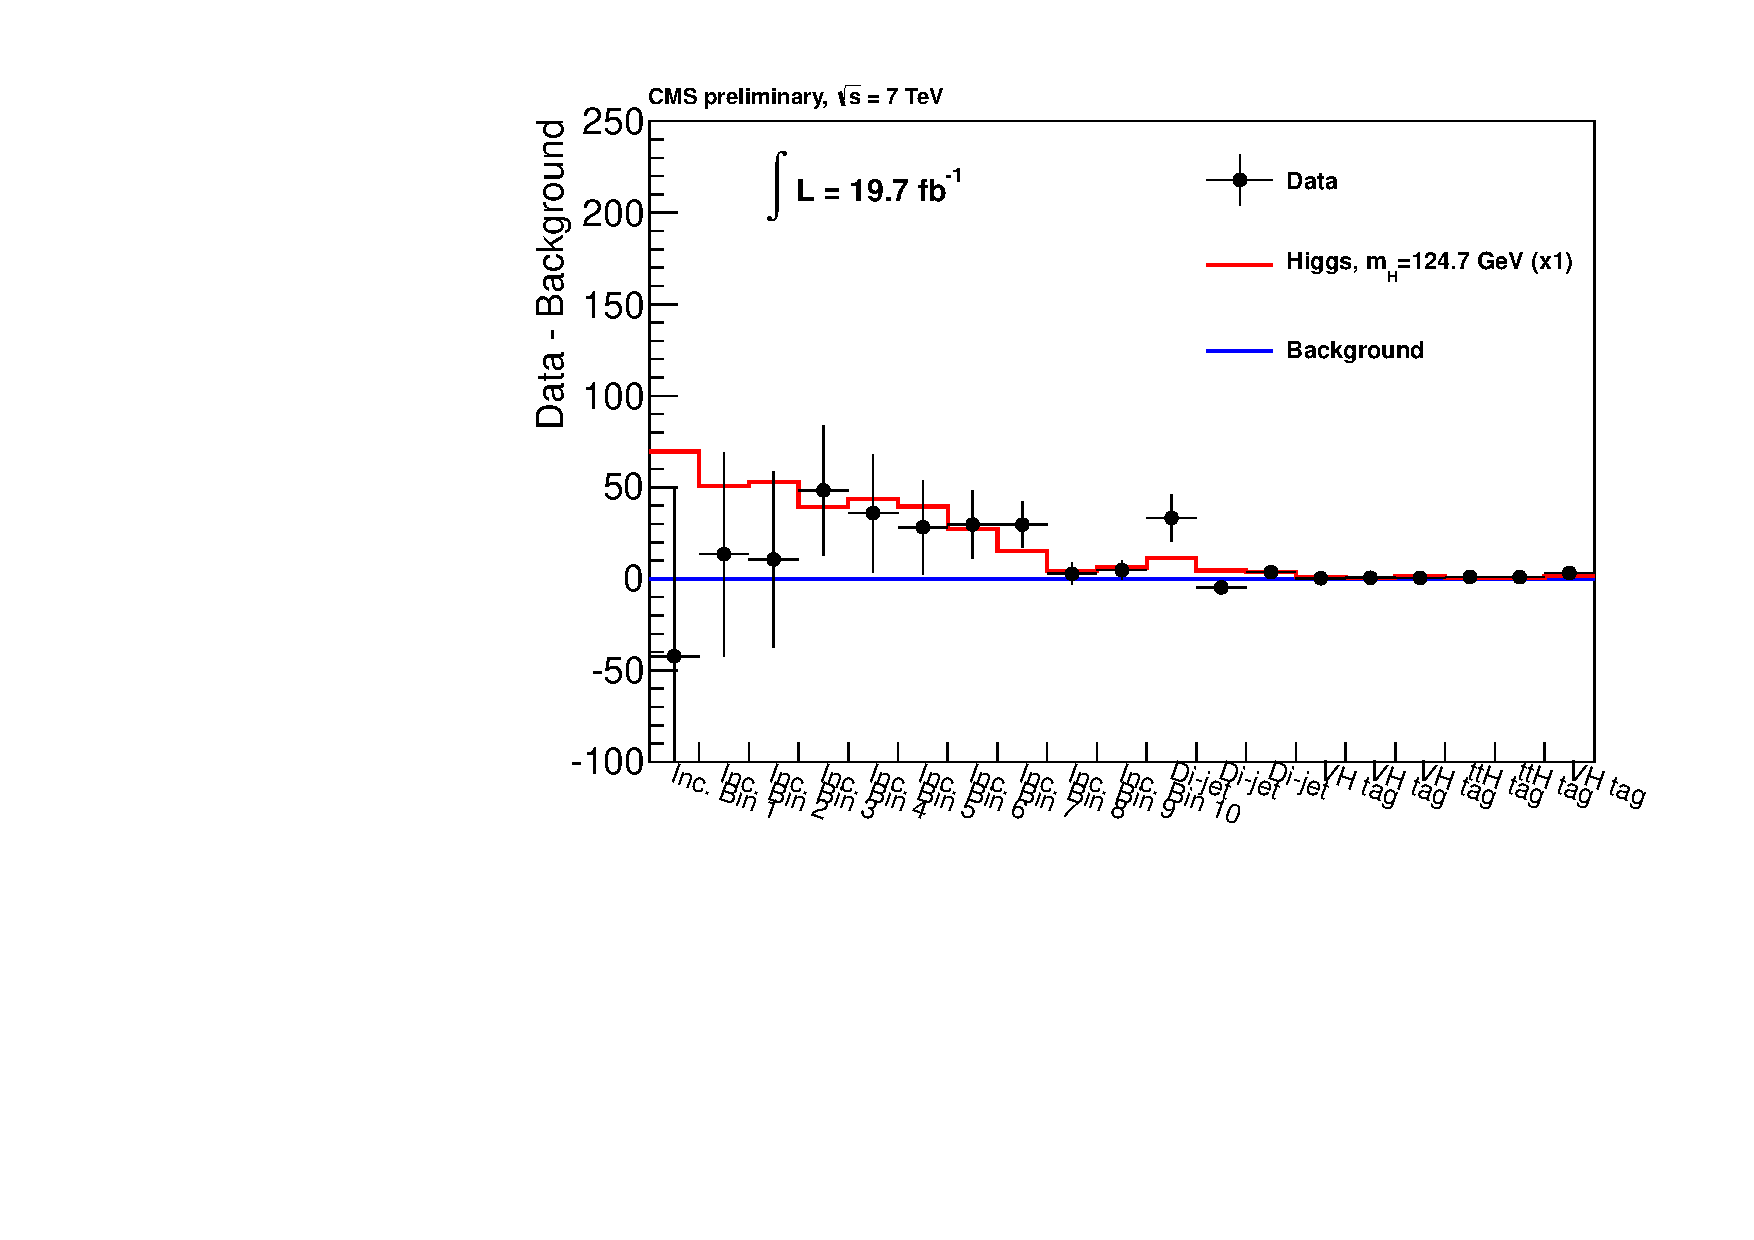
\includegraphics[width=0.48\textwidth]{{ch5_anal_and_results/plots/sideband/diff_model_8TeV_m124.7}.pdf}
  \caption{The distribution in sideband analysis bins for the data (black points), the background (blue line), the error on the background (green and yellow bands) and the signal (red line) for the mass hypothesis at \mH=124.7~\GeV. The top row shows the expected number of events of each type for the 7~\TeV (left) and 8~\TeV (right) datasets. The bottom row shows the background subtracted plot for data (black points) and signal (red line).}
  \label{fig:sideband_output}
\end{figure}


% ---- SECTION ----
\section{Systematic Uncertainties}
\label{sec:systematics}

There are several sources of systematic uncertainty in the analysis and these are described in the following section. These come in three borad categories; those associated to individual photons, those associated to events individual events, those associated to specific tagged event classes. The first type, those associated to individual photons, are implemented as Gaussian nuisance parameters which affect the position, shape and normalisation of the signal. The latter two types are implemented as log normal nuisance parameters which affect the normalisation of the signal and the relative signal yield in each event class. Log normal constraints are chosen for the latter so that the nuisance term cannot go negative.

\subsection{Systematic uncertainties related to individual photon errors}

These uncertainties are applied to individual photons and their affect is propagated through to the invariant mass shape and normalization of the signal for each production process and event class. The methodology for this is as follows,

\begin{itemize}
  \item Each uncertainty is designed to address a specific class of photons with similar properties. For example one uncertainty might be the energy scale uncertainty for unconverted photons in the barrel. We can label this class $c$ and the uncertainty for this class $\theta_{c}$ which is the nuisance parameter that gets implemented in the signal model.
  \item Within the class $c$ there may be several sub groups of photons which have different uncertainties. For example photons in the central barrel and outer barrel. We will label this uncertainty as $\sigma_{s}$.
  \item The full analysis is run through with each photon in class $c$ given a random shift by its individual uncertainty $\sigma_{s}$ and all other photons left alone 
  \item 
\end{itemize}


Because the final event classes contain mixtures of photons from several different regions (in \eta and \rnine) the full correlation between the individual photon uncertainties is mapped onto the final invariant mass signal shape of each analysis category.  

\textit{Photon energy scale}
In Section~\ref{sec:photon_energy} a method for correcting the photon energy using \Zee decays was described. Although the statistical uncertainties on these corrections is small, there are some data/\MC discrepancies that gives rise to a systematic uncertainty. This uncertainty is individually calculated for the 8 categories (4 in \eta and 2 in \rnine) for which the energy scale correction is applied. The uncertainty is then propagated   

\textit{Photon energy resolution}

\section{Statistics}
\subsection{Use of the Likelihood function as a test statistic}

\section{Results of the mass factorised analysis}

\section{Results of the sideband analysis}
